%\author{{ Dante Donati}\thanks{Columbia Business School and CESifo; dd3137@gsb.columbia.edu;} \hspace{85pt} {Nandan Rao}\thanks{Virtual Lab and UAB}
% \vspace{5pt}
%\\ { Victor Orozco-Olvera}\thanks{DIME, The World Bank} \hspace{25pt} {Ana Maria Muñoz Boudet}\thanks{Gender Group, The World Bank}\vspace{5pt}}

\vspace{-0.5cm}

\clearpage
\section{Introduction}
With over 60 percent of the world's population active on social media \citep{wearesocial2025}, governments and organizations increasingly rely on these platforms in social marketing campaigns to influence individuals’ beliefs, attitudes, and real-world behaviors.\footnote{Social marketing entails applying commercial marketing techniques to influence the behavior of target audiences to enhance personal welfare and societal well-being (\citealt{kotler1971social, andreasen1994social}).} The effectiveness of such campaigns is typically assessed using online engagement and direct-response metrics---such as likes, clicks, and website visits---as well as ``Brand Lift'' surveys that capture short-term effects (\citealt{atheycovid2023, Shawky2019}). While these methods may be appropriate for evaluating commercial outcomes such as purchase intent or sales (e.g., \citealt{bart2014products, johnson2017less}), they are often inadequate for assessing the longer-term goals of public-interest campaigns, such as those promoting public health, whose objectives depend on sustained changes in offline behavior that cannot be captured through platform metrics alone.
%. Because these campaigns aim to change offline behavior, their evaluation also requires outcome measures that cannot be captured through platform metrics alone and often depend on offline data.

Beyond measuring effectiveness, another challenge is that ad delivery on social media platforms is often optimized for engagement and cost efficiency rather than for the offline outcomes these campaigns are intended to influence. As a result, even effective messages may be shown disproportionately to users who are more likely to engage or are cheaper to reach, rather than to those for whom the intervention would generate the greatest health benefits (\citealt{lambrecht2019algorithmic, sapiezynski2022algorithms, gordon2021inefficiencies}). These concerns have become more salient as changes in privacy regulation and platform policies have reduced access to third-party targeting information and made independent evaluation more difficult (\citealt{johnson2020consumer, goldfarb2011privacy}).



This paper studies these measurement and delivery challenges in the context of a nationwide malaria-prevention campaign run on Facebook and Instagram in India. Using a district-level cluster-randomized design, original survey data, and administrative health-facility records, we estimate the causal effect of assignment to potential campaign exposure on offline behaviors and health outcomes, including bednet use, treatment-seeking, and malaria incidence. We then examine whether engagement-based delivery aligned with the campaign’s public-health objectives and use a follow-up individual-level experiment to distinguish limits of message delivery from limits of message content.

Malaria is transmitted by the bite of infected mosquitoes and disproportionately affects poor and rural populations \citep{dev2004physiographic}. The campaign, designed by the public-health NGO Malaria No More (MNM), used behaviorally informed messages to raise malaria awareness and promote both preventive behaviors (e.g., sleeping under mosquito nets) and response behaviors (e.g., seeking timely treatment).\footnote{For example, 75\% of households in our baseline survey own mosquito nets, but only 70\% of those households report using them regularly, implying that a substantial share remains at least partially unprotected.} The campaign ran for six months on Meta platforms and was optimized for engagement with the ads and MNM’s pages. Although this strategy generated substantial platform activity---reaching 130 million people, generating 46 million reactions across 22 Indian states, and delivering an average of 3.6 exposures per user at a total cost of US\$202{,}000---it remains unclear whether it translated into changes in offline behavior and health outcomes.



We focus on three high-malaria-incidence states---Uttar Pradesh, Jharkhand, and Chhattisgarh. As part of our formative research, we administered a scoping survey to social media users recruited through Facebook and Instagram ads, offering mobile credit as an incentive. The survey helped us identify 80 districts in which recruitment through social media was feasible within the study budget and provided information on household socioeconomic conditions and malaria-related risk characteristics that we used to balance treatment assignment across districts. We then partnered with the MNM advertising team to implement a cluster-randomized controlled trial in these districts, randomly assigning half to treatment. To preserve external validity, treated districts received the same advertising content and delivery strategy used in the nationwide campaign. Importantly, MNM relied on standard platform targeting based on available sociodemographic characteristics and optimized delivery for engagement. 


To measure the effects of the campaign, we recruited 8,253 individuals across the study districts. Specifically, we recruited respondents into a longitudinal sample ($N=5{,}201$) to study outcomes during the intervention period and into a cross-sectional sample ($N=3{,}052$) to study outcomes one to three months after the campaign ended. Because respondents in treated districts were not necessarily exposed to the ads, our survey-based estimates capture intent-to-treat effects for populations with a social-media presence.

In the longitudinal sample, data were collected using an experience-sampling design, with repeated observations approximately every 17 days over the course of the campaign. Across pooled and panel specifications, the estimated effects on bednet use among households owning at least one bednet are positive but imprecisely estimated. For other protective behaviors, as well as for self-reported fever, timely care-seeking, malaria incidence, and malaria testing during the campaign, we find no evidence of detectable average effects. In the cross-sectional sample, which measures outcomes after the campaign ended, the average effects are similarly limited: we do not detect clear changes in self-reported malaria incidence in the full sample, although we do find some evidence of increased bednet retreatment with insecticide among bednet owners.


We next examine, in a post-hoc manner, whether the campaign’s effects varied by baseline household socioeconomic status (SES). It is important to clarify that SES is used here to describe heterogeneity in treatment effects, not to isolate any single underlying channel. The index bundles housing conditions, access to health facilities, education, caste status, household size, and other correlated characteristics, some observed and others potentially unobserved, that may shape social-media use, digital engagement, and responses to health messages. At the same time, SES is negatively associated with baseline malaria incidence in our data, making it a useful summary measure for studying whether the campaign’s effects differed across groups that were ex ante more and less vulnerable to malaria risk. The results suggest that the campaign’s detectable effects were more concentrated among higher-SES households, defined as those above the median of the SES distribution. In particular, during the campaign, bednet use rose by 6.7 percentage points (p.p.) among higher-SES households, corresponding to an 11\% increase relative to the control mean, while the estimate for lower-SES households is small and statistically insignificant. After the campaign ended, malaria incidence fell by 0.9 p.p. among higher-SES households, a 56\% reduction relative to the control mean, whereas the corresponding estimate for lower-SES households is again small and statistically insignificant. For bednet retreatment with insecticide, the estimates point in the same direction, with a statistically significant increase only among higher-SES households.


We complement the survey evidence with administrative health-facility data from the Indian Health Management Information System (HMIS), which provide an objective measure of malaria incidence at the population level. In pooled specifications across all facilities, the estimated effects on malaria incidence are negative but imprecisely estimated. When we disaggregate by facility type, however, a clearer pattern emerges. Over the nine months following the launch of the campaign, monthly malaria incidence in urban health facilities in treated subdistricts declined by 6.2 cases per million people relative to the control group, corresponding to about 33\% of the average pre-treatment urban incidence rate. By contrast, we do not detect corresponding effects in rural areas. The campaign did not affect the number of malaria tests conducted, although the urban test positivity rate fell by about 2 percentage points. A similar urban-rural contrast persists in subdistricts with higher internet penetration, suggesting that internet access alone is unlikely to explain the rural null effects.

Taken together, the survey and administrative evidence point to limited average effects of the campaign. At the same time, post-hoc heterogeneity analyses suggest that the campaign’s detectable impacts were more concentrated among relatively advantaged households and in urban areas, while we find little evidence of impacts among poorer and rural populations, which face higher malaria risk. This raises a central question: do these patterns reflect lower effectiveness of the ad content, or lower exposure to the campaign?

On the one hand, the campaign content may have been less persuasive for poorer and higher-risk populations, reflecting limitations in the identification of relevant personas or in the tailoring of campaign messages. On the other hand, these populations may simply have been less likely to receive the ads---for example, because platform delivery algorithms prioritized users with higher expected engagement \citep{lambrecht2019algorithmic,sapiezynski2022algorithms}---which would instead point to limitations in targeting and delivery.

To shed light on these mechanisms, we rely on two complementary exercises. First, we study post-campaign ad recall, which provides suggestive evidence on differential exposure: if exposure differed systematically across groups, recall would be expected to differ as well. In the endline survey, treated respondents were 3 p.p. more likely to recall the campaign overall, corresponding to a 26\% increase relative to the control mean. When we split the sample by SES, recall rises by 4.7 p.p. among higher-SES respondents, compared with a statistically insignificant 1 p.p. among lower-SES respondents. We view this evidence as suggestive rather than conclusive, since recall is an imperfect proxy for exposure and may also reflect differences in attention or memory. 


Second, we implement a small-scale individual-level \textit{feed} experiment in which assignment to a remarketing campaign was randomized and the campaign reached most treated respondents, making ad delivery and exposure more comparable across SES groups. Between March and April 2021, after the nationwide campaign had ended, we used Meta’s Custom Audience tool to assign respondents to an individual-level remarketing campaign run by MNM on Facebook and Instagram. The campaign lasted two weeks, reached about 90\% of the target audience at least once, and delivered an average frequency of 4.9 ads per person. Two weeks later, we administered a follow-up survey ($N=1{,}542$). The campaign increased bednet use by 6.9 p.p. and timely treatment-seeking intentions by 2.5 p.p., with no evidence that these effects differed by SES. %Taken together, these results point more toward differential exposure to the nationwide campaign, than toward lower content effectiveness among disadvantaged populations. 


Taken together, our results suggest that the ad content can affect malaria-related behaviors among users reached by the ads, including lower-SES respondents in the individual-level experiment. The limited average effects of the nationwide campaign are therefore more consistent with targeting and delivery frictions than with uniformly low content effectiveness. Under engagement-based delivery, lower-SES, rural, or otherwise higher-risk users may have been less likely or more costly to reach. This could reflect lower social-media use, smaller reachable audiences, poorer internet connectivity, or differences between higher-risk users on the platform and higher-risk users in the broader population. Consistent with this interpretation, our district-level analysis shows that recruitment advertising was cheaper in larger and more populous districts, and in districts that were more socioeconomically advantaged and had greater mobile-phone penetration. Because the recruitment ads were also optimized for engagement-related objectives, much like the nationwide campaign, these cost patterns are informative about likely delivery dynamics. They suggest that engagement- and cost-based delivery tilted exposure toward relatively advantaged populations, although we cannot separately identify the precise source of this differential exposure.

A cost-effectiveness analysis based on administrative data shows that the cost per officially reported malaria case averted ranges from about US\$3.40 in urban areas to US\$6.50 overall. Because the true number of malaria cases in India is estimated to be substantially higher than the officially reported number \citep{world2021malaria}, the cost per estimated case averted could be considerably lower. Overall, our findings suggest that social media campaigns can be cost-effective public-health tools, but engagement-maximizing delivery may not direct exposure toward those with the highest expected health gains. More deliberate targeting may therefore be necessary if such campaigns are to reach the populations most in need of the intervention.

At the same time, our evidence offers a more cautious assessment of campaign effectiveness than studies based on immediate post-exposure surveys or Brand Lift designs, such as \citet{atheycovid2023}. A likely reason is that we estimate intent-to-treat effects at the population level, rather than effects conditional on ad exposure, and we focus on medium-term off-platform behaviors and health outcomes rather than on short-term shifts in recall, beliefs, or intentions measured immediately after exposure. In that sense, our results suggest that ad recall and immediate post-exposure surveys may provide an incomplete picture of the real-world impact of public-health campaigns delivered through social media.

The rest of the paper proceeds as follows. Section 2 describes the paper’s contribution to the literature. Section 3 provides background on the campaign and the intervention. Section 4 outlines the study design, and Section 5 describes the data. Section 6 presents the main results, and Section 7 examines the roles of content effectiveness and ad exposure. Section 8 discusses the implications of the findings, Section 9 presents the cost-effectiveness analysis, and Section 10 concludes.




\section{Contribution to the Literature}

A growing marketing literature studies the effectiveness of display advertising, documenting positive effects on brand and performance outcomes (\citealt{goldfarb2011privacy, lewis2014online, johnson2017less, bart2014products}) as well as important inefficiencies and measurement challenges (\citealt{gordon2021inefficiencies, johnson2023inferno}). We contribute to this literature by studying advertising effects on off-platform, socially relevant outcomes rather than traditional marketing metrics, and by developing an empirical design that combines randomized variation in campaign delivery with survey and administrative data to measure medium-term behavioral and health outcomes. 

More specifically, the paper relates to recent work on advertising campaigns with public-health objectives in both developed and developing-country settings. Digital and social media campaigns have been shown to affect alcohol and tobacco use (\citealt{wang2021investigating, thompson2013impact}), vaccination attitudes and behavior (\citealt{atheycovid2023, evans2023outcomes}), physical and eating habits (\citealt{carins2014eating}), and stigma reduction (see \citealt{Shawky2019}).\footnote{Mass-media campaigns have also been shown to improve health outcomes \citep{Orozco-Olvera2023}.} Relative to this literature, our main contribution is to evaluate a social media campaign using off-platform outcomes measured over a longer horizon. Rather than relying on engagement metrics or short-term Brand Lift surveys,\footnote{Brand Lift studies, offered by platforms such as Meta and Google, typically measure recall, sentiment, and purchase intent using short surveys administered shortly after ad exposure.} we track malaria-related behaviors and disease outcomes for up to five months following potential exposure. This difference in estimand and measurement horizon yields a more cautious assessment of campaign effectiveness than studies based on immediate post-exposure surveys alone. 

Our results also contribute to the literature on algorithmic targeting and ad delivery. Consistent with prior work (\citealt{lambrecht2019algorithmic, sapiezynski2022algorithms}), we show that optimizing delivery for engagement can create a tension between platform performance and real-world impact. The combination of post-campaign recall, the individual-level feed experiment, and district-level correlates of ad costs points to targeting and delivery frictions as an important constraint on campaign effectiveness. In particular, our evidence suggests that engagement- and cost-based delivery may tilt exposure toward users and places that are easier and cheaper to reach, rather than toward those with the highest expected health gains, although we cannot isolate the exact source of this differential exposure. More broadly, our study also complements field-based evaluations of traditional malaria interventions—such as the subsidized distribution of antimalarials, rapid diagnostic tests, and insecticide-treated bednets (\citealt{cohen2015price, tarozzi2014micro})—by showing what social media campaigns can and cannot achieve when the intervention works through information and platform delivery rather than through the direct provision of prevention or treatment tools.

The paper further speaks to the role of data in both targeting and measurement, and thus to the broader privacy debate in digital marketing (\citealt{acquisti2016economics, tucker2018privacy}). Our design shows how first-party survey data collected from social media users can be used to evaluate campaign effects and to inform targeting while limiting reliance on third-party data. In that sense, the paper offers practical guidance for the use of marketing analytics in public-policy settings (\citealt{davis2021future}) and for the design of social media campaigns when privacy and measurement constraints make conventional targeting more difficult. 

Finally, the paper contributes to a broader literature on marketing for social impact (\citealt{chandy2021better, kotler1971social}), especially in emerging-market settings \citep{narasimhan2015marketing}. Related work studies consumer literacy (\citealt{viswanathan2021marketplace}), environmental behavior (\citealt{sun2021buy, zhang2021social, brecko2023pro}), gender norms and violence prevention (\citealt{donati2022}), managerial and marketing skills (\citealt{anderson2018pathways, bulte2017gender}), technology diffusion through networks (\citealt{miller2015learning}), and social norms as tools for behavior change (\citealt{burchell2013marketing}). Our study adds to this literature by showing both the promise and the limits of social media advertising as a tool for public-health interventions at scale.






\section{Background and Intervention}

\subsection{Malaria and COVID-19 in India}

Malaria is a mosquito-borne disease caused by parasites and transmitted through the bite of infected mosquitoes. As in many other countries, malaria incidence in India has declined substantially over the last two decades: the number of cases per 1,000 population at risk fell from 19.9 in 2000 to 3.2 in 2020 \citep{worldbankdata2022}. Despite this progress, malaria remains an important public health challenge. An estimated 93\% of India’s population lives in areas at risk of malaria \citep{world2018malaria}. In 2020, the disease caused about 7,300 deaths and an estimated 4.1 million cases, of which only around 186,000 were officially recorded---roughly one in every 22 cases \citep{world2021malaria}. This large gap likely reflects a combination of under-reporting, asymptomatic infections, limited access to care, and diagnostic constraints. Malaria also disproportionately affects poorer and rural populations \citep{dev2004physiographic}, and each episode is estimated to result in 11 lost days of work or school \citep{singh2019economic}.

The malaria prevention campaign ran from August 2020 to January 2021, during the first year of the COVID-19 pandemic. This was a period of major disruption to India’s health system, including reduced availability of routine services such as malaria testing and treatment. Public health guidance to limit movement and avoid healthcare facilities may have further discouraged care-seeking. At the same time, the overall effect of the pandemic on malaria-related service demand is ambiguous. Reduced mobility and fear of infection may have lowered testing, whereas the expansion of COVID-19 testing and the overlap between malaria and COVID-19 symptoms may have increased the perceived value of diagnostic care. More time spent at home may also have increased time spent online, potentially affecting ad exposure and engagement. These countervailing forces may limit the external validity of our findings, but they are unlikely to threaten the internal validity of the experimental design.




\subsection{Social Media Use in India} \label{sec_intervention}

As of December 2020, the average Indian user spent approximately 2.5 hours per day on social media.\footnote{These metrics come from https://napoleoncat.com/stats/social-media-users-in-india/2020/ and https://datareportal.com/reports/digital-2021-india, accessed in May 2025.} Although platforms such as Instagram and TikTok had become increasingly popular among younger audiences globally, Facebook remained a primary social media channel for young adults in India during our study period. It had 392 million active users, corresponding to 26.7\% of the total population. Around 70\% of these users were between ages 18 and 34, and another 21\% were between 35 and 64. The platform also exhibited a marked gender imbalance, with about 75\% of users identifying as male. Facebook Messenger, which we used to administer our surveys, had comparable penetration and demographic patterns. Instagram had 137 million users, 76\% of whom were between 18 and 34 years old. TikTok was also widely used in early 2020, but it was banned in India in June of that year and remained inaccessible during the period of our study.


\subsection{The Ad Campaign and Its Content} 

The evaluated malaria-prevention campaign, titled \textit{Bite Ko Mat Lo Lite} (``Don’t Take the Bite Lightly''), was a national initiative implemented across 22 high-malaria-incidence states in India, covering 86\% of the country’s population. Although our impact evaluation focuses on three states, the campaign content and delivery strategy in those states mirrored the broader national rollout. 

The campaign ran on Facebook and Instagram during the monsoon season and the following months, when malaria transmission is typically elevated. It was designed and implemented by Malaria No More (MNM), an international nonprofit, with support from Facebook’s Campaigns for a Healthier World initiative, which provided advertising credits, and from Upswell, a social media marketing firm that provided technical assistance. The evaluation team had no role in designing or managing the campaign.

Rather than encouraging costly household investments or collective prevention efforts, the campaign focused on simple actions individuals could take on their own. Its main objectives were to increase consistent bednet use and to encourage early diagnosis and treatment-seeking in response to fever. Some ads also mentioned other preventive measures, such as wearing long sleeves or using repellents, but bednet use and prompt care-seeking remained the campaign's main behavioral targets. These behaviors are central to malaria policy and research, as reflected in WHO and Indian guidance and in a broad literature on insecticide-treated nets and malaria-related behavior change \citep{lengeler2004insecticide, cohen2010free, koenker2014strategic, world2025guidelines}.\footnote{This emphasis is also consistent with Indian malaria policy: the National Framework for Malaria Elimination highlights mosquito nets, prompt diagnosis, and early treatment as key malaria-control tools \citep{india2016nfme}. Basic mosquito nets in India cost about \$1.5--\$5, making them affordable for many households.}



The campaign content was informed by two complementary frameworks. First, MNM adopted a persona-based segmentation approach, creating six audience personas that varied by age, gender, and urban versus rural location. These personas were developed using focus groups and were used to tailor language, imagery, and tone across ads.\footnote{Details on persona development and examples of the creatives are provided in Annex \ref{mal-appendix:A}. For example, humorous and meme-styled content was developed for younger audiences, whereas ads aimed at older audiences emphasized family roles and the importance of involving other household members in testing and prevention.} Second, the campaign drew on standard health-behavior principles, especially the idea that behavior change is more likely when messages increase motivation, make the recommended action seem feasible, and provide clear prompts to act \citep{fogg2009behavior}. In practice, the ads emphasized the risks posed by malaria, framed prevention and treatment as manageable everyday actions, and used direct calls to action.\footnote{For example, one ad depicted parents putting their child to sleep while conveying that ``Getting them treated on time is as important as making them sleep on time,'' thereby presenting timely care-seeking as a routine and feasible action. Other ads used explicit prompts such as ``If you notice signs of fever, see a doctor immediately'' and ``Protect your children from mosquito diseases, always use mosquito nets.''}

\subsection{Campaign Delivery and Engagement Optimization}


Campaign delivery took place in two phases. In the first phase, from July to November 2020, MNM used Meta Ad Manager to run a single campaign with the explicit objective of maximizing engagement. The campaign was organized into six ad sets, each corresponding to one of the six personas. Within each ad set, MNM initially placed the creatives designed for that persona. Based on early engagement metrics---including clicks, comments, and reactions---lower-performing ads were turned off and budget was reallocated toward higher-performing creatives. During the first weeks of the campaign, this process narrowed the active set of creatives to 22 ads focused on the campaign’s core messages, which together accounted for at least 73\% of total spending.\footnote{While we do not observe the full initial set of creatives, an MNM report documents the 22 ads retained during the streamlining process; see Annex Figures \ref{fig:women} to \ref{fig:top_content}. Most emphasized bednet use, mosquito risk, and timely treatment-seeking. Only one focused on malaria symptoms, and just two recommended the use of mosquito repellents.} This streamlining concentrated attention on a small number of behaviors that the campaign sought to make salient and actionable.

In the second phase, from December 2020 to January 2021, MNM again ran a campaign with the objective of maximizing engagement. The campaign retained the same six persona-based ad sets, but these were now populated with the top-performing creatives from the first phase rather than only with creatives tailored to each persona. As a result, in the later phase of the campaign, all target audiences could receive the creatives that had generated the strongest engagement earlier in the rollout.

This delivery strategy is important for interpreting our results. For a public-health campaign, optimizing for engagement is an imperfect objective because it can shift delivery toward users who are more likely to click or react online, rather than toward those for whom the expected health gains are greatest. In our setting, MNM used broad demographic targeting criteria based on the personas and then relied on Meta’s algorithm to optimize delivery within those groups. As a result, conditional on being in a targeted audience, the intensity---and likely the mix---of ad exposure was shaped by platform-side engagement patterns that were not observed by the research team.

The same delivery strategy was used in the treated districts in our study. On average, the campaign generated 3.6 impressions per reached individual, with peaks of about five, and produced more than 45 million actions, including clicks, likes, and comments. Although we do not observe individual-level exposure to specific creatives,\footnote{We do not observe creative-level exposure by geography. Given the broad targeting criteria and the demographic diversity of treated districts, however, the mix of content delivered in the study areas likely resembled that of the national campaign.} our design allows us to estimate the intent-to-treat effect of the campaign as implemented in practice, rather than the effect of any specific ad.

 


\section{Study Design}

In coordination with the MNM team, we limited the study to three states---Uttar Pradesh, Chhattisgarh, and Jharkhand---where MNM agreed to postpone the launch of the nationwide campaign until late August 2020. These states resembled the other 19 campaign states on key malaria-burden indicators and had sufficiently high social media penetration. All three were high-burden settings with prior bednet distribution and previous MNM operations.

\subsection{District Selection and Sample Recruitment}

At the time of the intervention, the three study states comprised 126 districts with a combined population of more than 300 million. Based on power calculations and formative research, we selected 80 districts for inclusion in the study. One district was later dropped because of an implementation issue, leaving a final sample of 79 districts (data sources and processing are described in Table \ref{tab:data_cleaning}).

To identify the study districts, we first excluded the three state capitals, which were outliers on multiple dimensions. We then focused on the remaining 123 eligible districts and conducted formative research through a scoping survey in July and August 2020. Participants were recruited using Facebook and Instagram ads, as social media users were the population of interest for the study. Because Meta did not allow district-level ad targeting, we used GIS software to draw expanding circles around each district’s main cities, stopping at district boundaries. These geofenced areas defined the targeting zones for the recruitment ads. Respondents were offered mobile-phone credit (US\$2.60--3.60) and completed the survey through a Facebook Messenger chatbot hosted on a page we created called ``Global Insights'' (see Annex Figure \ref{fig:recruitment_ads}). The survey collected demographic and socioeconomic information, as well as measures of household malaria incidence over the previous five years and the previous two weeks. We also recorded recruitment advertising costs by district.



The scoping survey was also used to identify districts in which recruitment through social media was feasible within the study budget. In practice, this meant selecting districts with lower advertising costs---measured by cost per thousand impressions (CPM)---and higher ad engagement, as captured by click-through rates (CTR). This screening made it possible to recruit sufficiently large samples in each district, but it also yielded a socioeconomically skewed set of study districts. Annex Table \ref{tab:districts_characteristics_bystudy} shows that, relative to excluded districts, included districts had lower CPM, higher CTR, and lower cost per completed survey. They were also more socioeconomically advantaged, with larger populations and greater internet and mobile-phone penetration. Although this screening affects the socioeconomic composition of the study districts, included and excluded districts remain comparable in terms of self-reported recent malaria cases and administrative malaria positivity rates.

Table \ref{tab:correlates_recruitment} further examines district-level correlates of recruitment ad costs across included and excluded districts, reporting both bivariate regressions and a joint specification. The bivariate results show that lower recruitment CPM is associated with higher population density, larger population, a lower share of rural population, a higher share of households living in solid dwellings, greater wealth, and higher internet and mobile-phone access. In the joint specification, the predictors of lower recruitment CPM that remain significant at the 10\% level are larger population, a higher share of households living in solid dwellings, and a higher share of mobile-phone ownership. These patterns are informative for interpreting the later campaign results because the recruitment ads, like the nationwide malaria campaign, were delivered through engagement-optimized advertising.

\begin{table}[!htbp]
    \centering
    \caption{District-level correlates of recruitment advertising costs}
    \footnotesize
    \hspace*{-1.5cm}
    {
\def\sym#1{\ifmmode^{#1}\else\(^{#1}\)\fi}
\adjustbox{max width=\textwidth}{%
\begin{tabular}{l*{9}{c}}
\hline\hline
                &\multicolumn{9}{c}{\shortstack{Cost per mille, USD (mean CPM =     0.949)}}                                                                                               \\\cmidrule(lr){2-10}
                &\multicolumn{1}{c}{(1)}         &\multicolumn{1}{c}{(2)}         &\multicolumn{1}{c}{(3)}         &\multicolumn{1}{c}{(4)}         &\multicolumn{1}{c}{(5)}         &\multicolumn{1}{c}{(6)}         &\multicolumn{1}{c}{(7)}         &\multicolumn{1}{c}{(8)}         &\multicolumn{1}{c}{(9)}         \\
\hline
log(population density)&   -0.346\sym{***}&                  &                  &                  &                  &                  &                  &                  &                  \\
                &  (0.114)         &                  &                  &                  &                  &                  &                  &                  &                  \\
log(population) &                  &   -0.478\sym{***}&                  &                  &                  &                  &                  &                  &   -0.338\sym{**} \\
                &                  &  (0.133)         &                  &                  &                  &                  &                  &                  &  (0.145)         \\
log(area)       &                  &                  &    0.085         &                  &                  &                  &                  &                  &   -0.090         \\
                &                  &                  &  (0.080)         &                  &                  &                  &                  &                  &  (0.101)         \\
Share rural population&                  &                  &                  &    0.945\sym{***}&                  &                  &                  &                  &   -0.562         \\
                &                  &                  &                  &  (0.300)         &                  &                  &                  &                  &  (0.421)         \\
Share in solid houses&                  &                  &                  &                  &   -0.900\sym{***}&                  &                  &                  &   -0.656\sym{**} \\
                &                  &                  &                  &                  &  (0.291)         &                  &                  &                  &  (0.327)         \\
Wealth index    &                  &                  &                  &                  &                  &   -0.192\sym{***}&                  &                  &    0.097         \\
                &                  &                  &                  &                  &                  &  (0.061)         &                  &                  &  (0.060)         \\
Share with internet access&                  &                  &                  &                  &                  &                  &   -1.845\sym{***}&                  &   -0.652         \\
                &                  &                  &                  &                  &                  &                  &  (0.585)         &                  &  (0.411)         \\
Share with mobile phone&                  &                  &                  &                  &                  &                  &                  &   -5.198\sym{***}&   -2.847\sym{*}  \\
                &                  &                  &                  &                  &                  &                  &                  &  (1.702)         &  (1.603)         \\
Constant        &   -1.623\sym{**} &    1.263\sym{***}&    0.848\sym{***}&    0.225         &    1.290\sym{***}&    0.950\sym{***}&    1.847\sym{***}&    5.705\sym{***}&    4.877\sym{***}\\
                &  (0.816)         &  (0.118)         &  (0.074)         &  (0.202)         &  (0.148)         &  (0.045)         &  (0.318)         &  (1.589)         &  (1.621)         \\
\hline
Observations    &\num{117}         &\num{117}         &\num{117}         &\num{117}         &\num{117}         &\num{117}         &\num{117}         &\num{117}         &\num{117}         \\
Adj. R-squared  &    0.325         &    0.418         &   -0.003         &    0.099         &    0.069         &    0.129         &    0.189         &    0.383         &    0.466         \\
\hline\hline
\multicolumn{10}{p{1.12\linewidth}}{\scriptsize The table reports OLS coefficients from regressions of cost per mille (CPM), collected during the scoping survey, on district characteristics from DHS and UN data (2019--2021). Each observation is a district. The Wealth Index is provided by the DHS and comprises household assets and access to utilities and services. Only districts with complete data on the variables included in each specification are used. Heteroskedasticity-robust standard errors are reported in parentheses. \sym{*} \(p<0.1\), \sym{**} \(p<0.05\), \sym{***} \(p<0.01\).}\\
\end{tabular}
}%

}






    \label{tab:correlates_recruitment}
\end{table}

Once the study districts were selected, we conducted additional analysis to refine the sampling strategy and define stratification criteria. Our goal was to ensure meaningful variation in baseline socioeconomic conditions and malaria risk within the selected districts, so that the study could examine both average effects and heterogeneity across different types of connected households.

Table \ref{tab:malaria_correlates} reports pairwise correlations between malaria incidence and household-level characteristics using the sociodemographic data collected during formative research; Annex Table \ref{tab:malaria_predictors} reports the corresponding OLS regression estimates. Several characteristics are significantly associated with malaria incidence, including household size, distance to medical facilities, membership in socially disadvantaged castes, and dwelling type.\footnote{Following the India DHS survey, respondents reported living in one of three housing types: non-solid (e.g., mud, tin, straw), solid (durable materials like brick or concrete), or semi-solid (intermediate between the two).} To summarize broader household socioeconomic conditions, we construct an index of socioeconomic status (SES) following the standard Demographic and Health Surveys approach to household wealth measurement,\footnote{Details are available at: https://dhsprogram.com/topics/wealth-index/Wealth-Index-Construction.cfm} using principal component analysis of baseline household characteristics; column 3 of Table \ref{tab:malaria_correlates} reports the corresponding factor loadings. In line with prior research (e.g., \citealt{dev2004physiographic}), the index is strongly negatively associated with baseline malaria incidence: a one-standard-deviation increase in SES is associated with a 2.2 p.p. lower probability that any household member had malaria in the previous five years and a 0.4 p.p. lower probability of malaria in the previous two weeks.

\begin{table}[!htbp]
    \centering
    \caption{Pairwise correlations between malaria incidence, household characteristics, and SES index}
    \footnotesize
    {
\def\sym#1{\ifmmode^{#1}\else\(^{#1}\)\fi}
\adjustbox{max width=\textwidth}{%
\begin{tabular}{l*{2}{c}c}
\hline\hline
                &\multicolumn{1}{c}{(1)}&\multicolumn{1}{c}{(2)}&\multicolumn{1}{c}{(3)}\\
                &\multicolumn{1}{c}{\shortstack{Any HH member had \\malaria in last 5 years}}
                &\multicolumn{1}{c}{\shortstack{Any HH member had \\malaria in last 2 weeks}}
                &\multicolumn{1}{c}{\shortstack{SES index: \\PC1 loadings}}\\
\hline
Solid house     &   -0.056\sym{***}&   -0.036\sym{***}&   0.6590\\
                & (0.0000)         & (0.0016)         &         \\
Semi-solid house&    0.031\sym{***}&    0.004         &  -0.5974\\
                & (0.0069)         & (0.7370)         &         \\
Within 60 min to health facility
                &   -0.038\sym{***}&   -0.032\sym{***}&   0.2596\\
                & (0.0009)         & (0.0049)         &         \\
University degree
                &    0.045\sym{***}&   -0.001         &   0.1959\\
                & (0.0001)         & (0.9621)         &         \\
Advantaged caste
                &   -0.043\sym{***}&   -0.027\sym{**} &   0.1602\\
                & (0.0002)         & (0.0190)         &         \\
Has air conditioning
                &   -0.023\sym{**} &    0.003         &   0.2661\\
                & (0.0423)         & (0.7967)         &         \\
Household size  &    0.048\sym{***}&    0.044\sym{***}&  -0.0810\\
                & (0.0000)         & (0.0001)         &         \\ \hline
\addlinespace SES index (PC1 score)
                &   -0.056\sym{***}&   -0.031\sym{***}&         \\
                & (0.0000)         & (0.0062)         &         \\
\addlinespace \hline
Observations    &     7548         &     7548         &         \\
\hline\hline
\multicolumn{4}{p{.98\linewidth}}{\scriptsize Notes: Columns (1) and (2) report Pearson correlation coefficients between baseline malaria incidence and SES components (standardized) as well as the SES index (PC1 score). Column (3) reports PCA loadings for the first principal component (PC1) used to construct the SES index. Baseline responses collected from July 23 to August 19, 2020 are included. \textit{p-values} in parentheses. \sym{*} \(p<0.1\), \sym{**} \(p<0.05\), \sym{***} \(p<0.01\).}\\
\end{tabular}
}%

}
    \label{tab:malaria_correlates}
\end{table}

To implement the stratification in practice, we used dwelling type, which could be measured with a single survey question during recruitment and provided a simple way to identify households that were more likely to be socioeconomically disadvantaged and at higher malaria risk. In our formative data, households living in solid dwellings had lower past and current malaria incidence than households living in non- and semi-solid homes.\footnote{This is consistent with prior findings in India \citep{yadav2014socio} and elsewhere \citep{wanzirah2015mind}.} We therefore used dwelling type as an operational recruitment variable, allocating more budget toward recruiting respondents in non- and semi-solid dwellings and monitoring sample composition in real time across districts. This helped ensure adequate representation of more vulnerable households in the survey samples while also facilitating comparison with the urban-rural split available in the administrative malaria data.



 
\subsection{Cluster-level Randomization and Balance Checks} \label{sec:cluster-design}
 
In coordination with MNM, we randomly assigned the campaign across districts in the three study states. Specifically, 39 of the 79 study districts were assigned to treatment (ads) and the remaining 40 to control (no ads), while balancing on a set of pre-intervention district characteristics. Beyond overseeing the randomization, the evaluation team had no role in campaign implementation.


\begin{figure}[h!]
    \centering
    \caption{Cluster-randomization of districts (and circles therein)}
    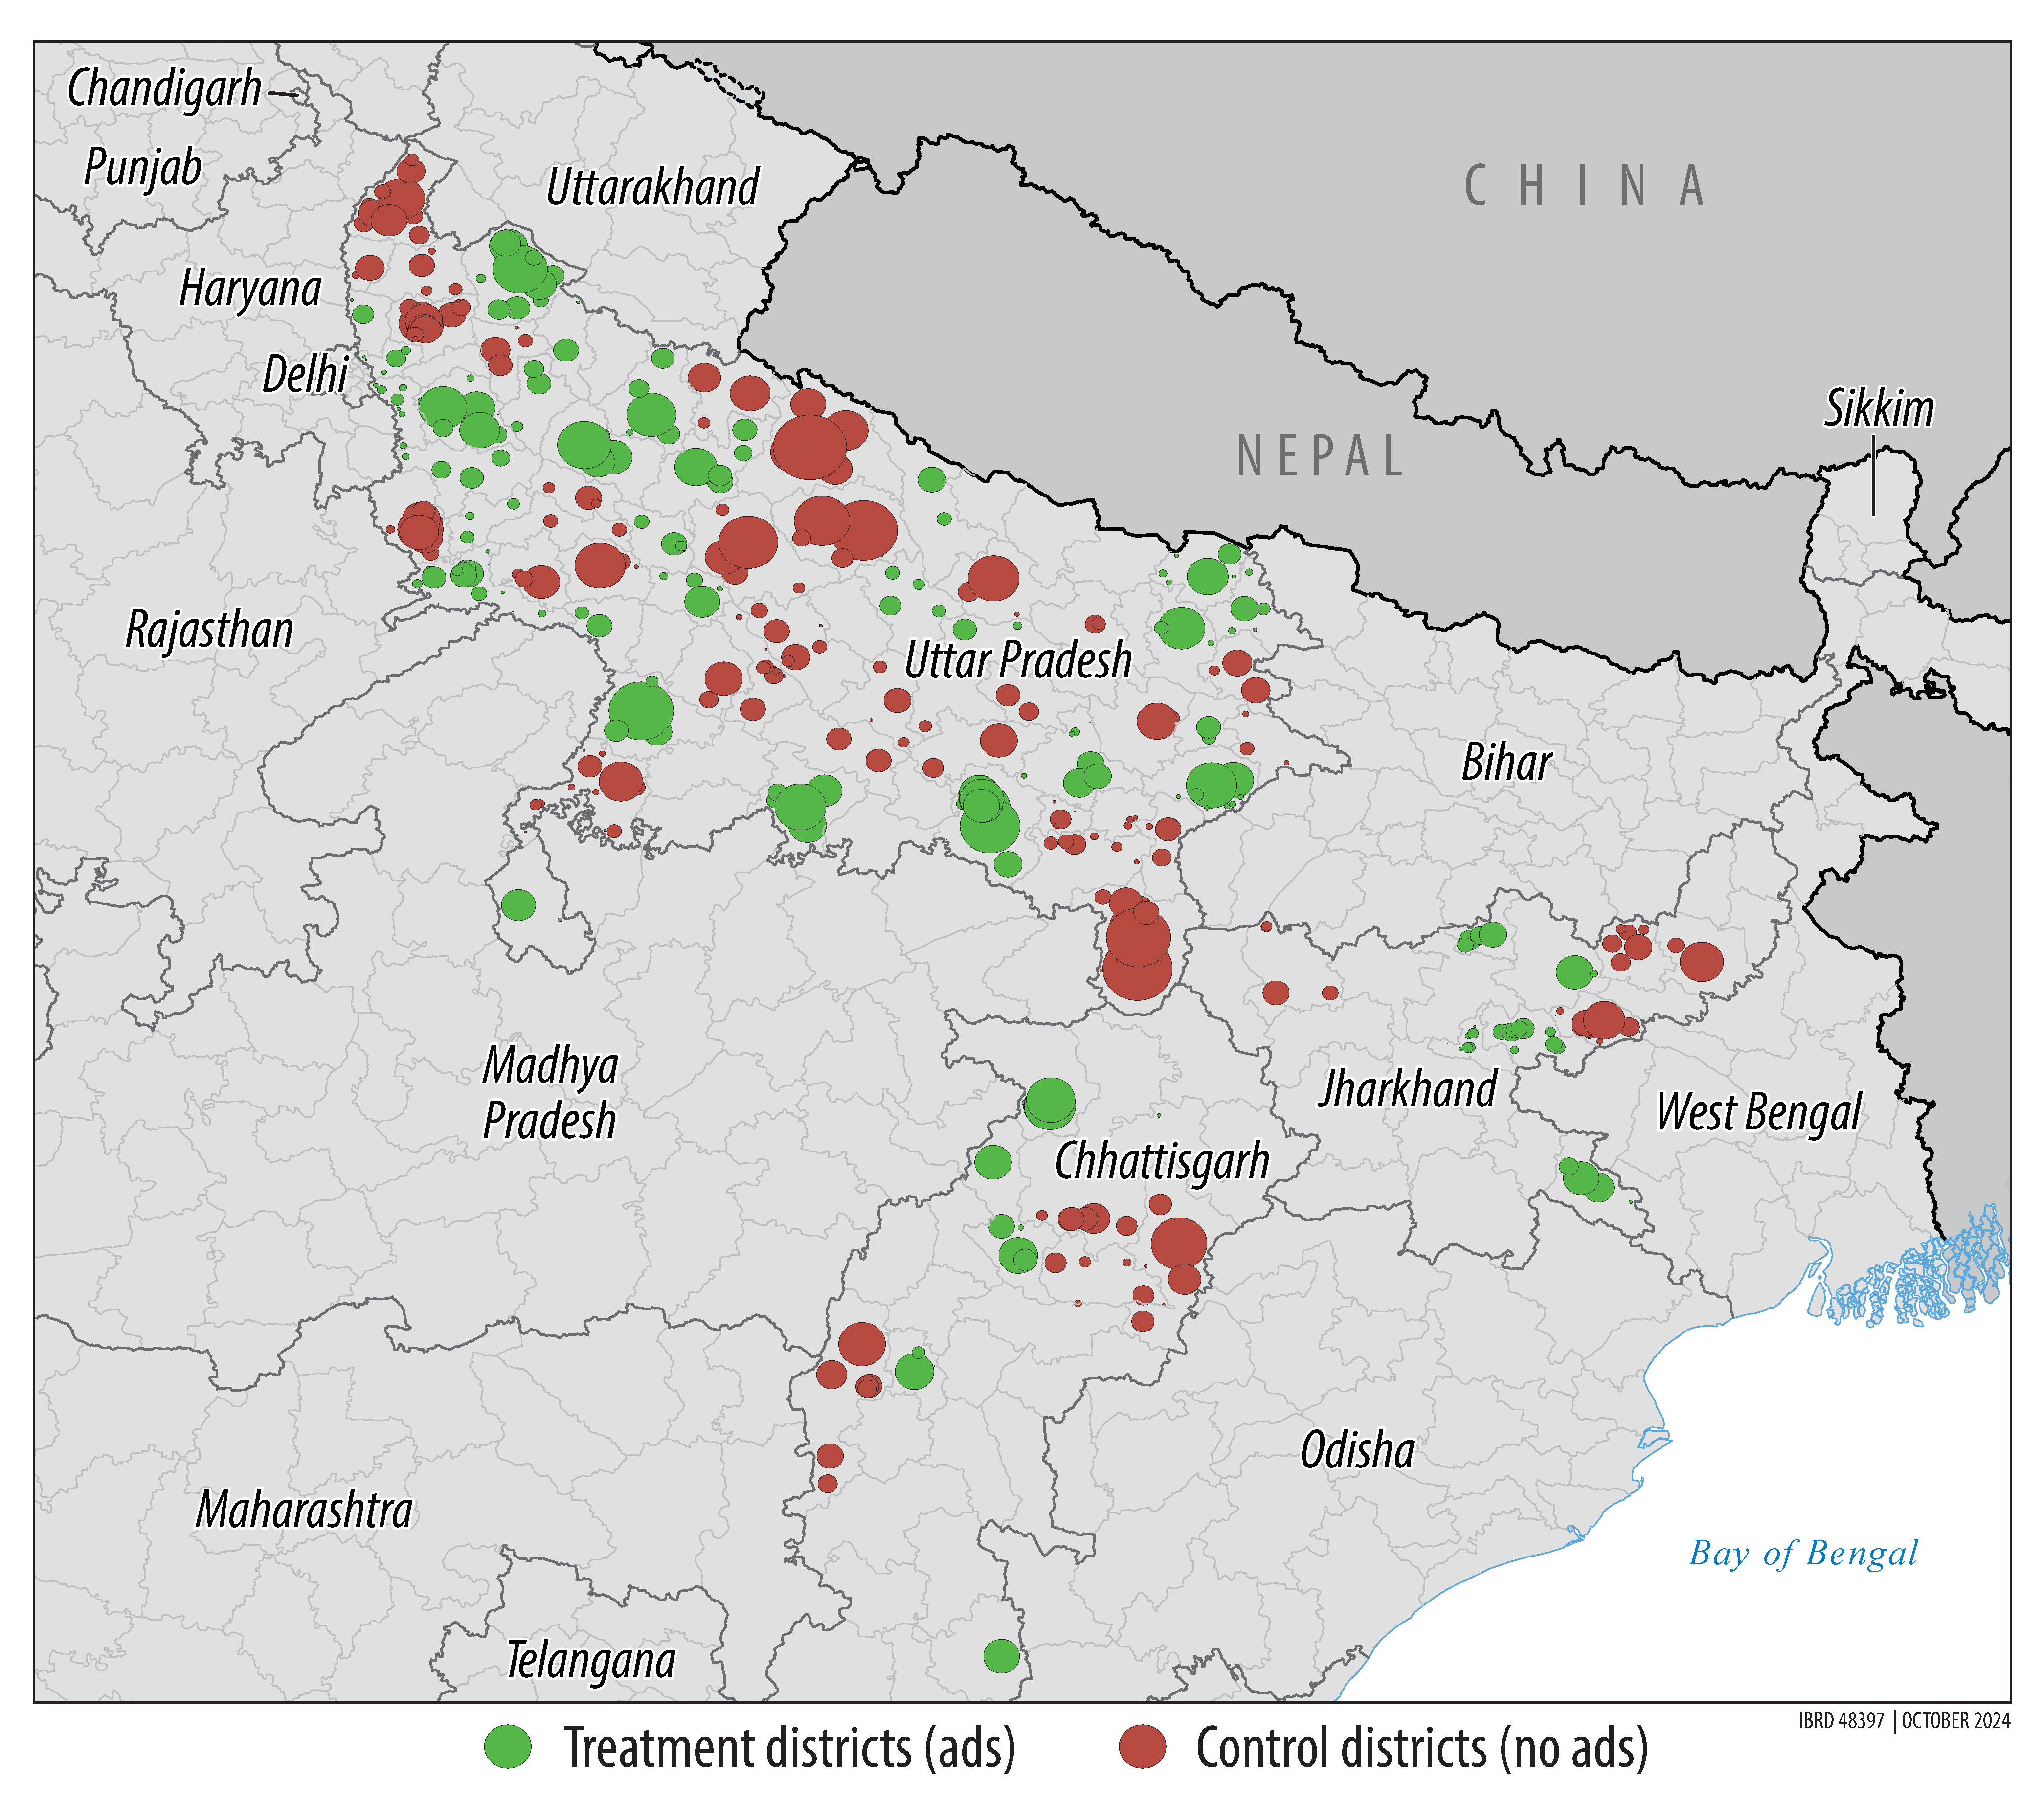
\includegraphics[scale=.14]{chapters/02-malaria/figures/clusters_wb.pdf}
    \label{fig:clusters}
    \begin{minipage}{16.5cm} \vspace{-0.4cm}
    
\includegraphics[scale=1]{chapters/02-malaria/figures/disclaimer_wb.pdf} \scriptsize {This map was produced by the Cartography Unit of the World Bank Group. The boundaries, colors, denominations and any other information shown on this map do not imply, on the part of the World Bank Group, any judgment on the legal status of any territory, or any endorsement or acceptance of such boundaries.}
\end{minipage}
\end{figure}

Figure \ref{fig:clusters} maps the treatment and control districts. The circles denote the geofenced areas used for both survey recruitment and campaign delivery. All circles within a district were assigned to the same experimental condition and were defined using their centroid coordinates and a fixed radius. We provided these geofenced areas to the MNM advertising team, which excluded the control circles (in red) from the nationwide campaign while delivering ads in the treatment circles (in green), as well as in other targeted areas and states. The cluster design offers two main advantages \citep{Hayes2017}. First, it accounts for potential spillovers---within households, across social networks (e.g., through shared Facebook content), and through reduced malaria transmission among neighbors---while limiting contamination between treatment and control areas. Second, it allows us to study not only individual-level effects in the survey data but also broader population-level effects in administrative health records, including the effects of collective behavior change on local malaria incidence.

\begin{table}[h!]
    \centering
    \caption{District characteristics by experimental condition} 
     \footnotesize
    \adjustbox{max width=\textwidth}{%
\begin{tabular}{lccccc}
\hline  & Treatment & Control & Normalized & \it T-test & \\
 & \it Mean & \it Mean & Difference & (\it p-value) & \\
 & (1) & (2) & (3) & (4) & \\
\hline \textbf{N. of districts} & 39 & 40 &  &  & \\  &  &  &  &  & \\[-5ex]\\
\textbf{A: Scoping survey (August 2020)} &  &  &  &  & \\
 &  &  &  &  & \\[-5ex]\\
Share living in solid houses & 0.502 & 0.494 & 0.078 & 0.623 & \\
Share with university degree & 0.598 & 0.593 & 0.063 & 0.693 & \\
Share unemployed & 0.439 & 0.446 & -0.103 & 0.519 & \\
Share with malaria in last 2 weeks & 0.017 & 0.016 & 0.072 & 0.652 & \\
Share with malaria in last 5 years & 0.190 & 0.184 & 0.051 & 0.750 & \\
Average click-through rate (\%) & 1.830 & 1.847 & -0.048 & 0.764 & \\
Average cost per mille (USD) & 0.764 & 0.758 & 0.050 & 0.756 & \\
Average ad cost per survey started (USD) & 0.252 & 0.241 & 0.072 & 0.650 & \\
Average ad cost per survey completed (USD) & 0.820 & 0.858 & -0.052 & 0.744 & \\
\hline \\[-5.1ex] &  &  &  &  & \\
 \textbf{B: Administrative sources (2011-2020)} &  &  &  &  & \\
 &  &  &  &  & \\[-5ex]\\
Area (thousand sq km) & 3.434 & 3.773 & -0.149 & 0.352 & \\
Population (millions, Census 2011) & 2.757 & 2.629 & 0.077 & 0.629 & \\
Population (millions, UN, 2020 estimate) & 2.978 & 2.906 & 0.040 & 0.804 & \\
Share of rural population (UN, 2020 estimate) & 0.687 & 0.732 & -0.174 & 0.278 & \\
Malaria positivity rate (Sep 2019 - Aug 2020) & 0.020 & 0.017 & 0.072 & 0.654 & \\
Household size & 5.821 & 5.833 & -0.013 & 0.934 & \\
Share of females & 0.478 & 0.479 & -0.065 & 0.685 & \\
Share of Hindu & 0.813 & 0.830 & -0.116 & 0.469 & \\
Share with age under 7 & 0.156 & 0.152 & 0.203 & 0.207 & \\
Socioeconomic Development Index & 0.048 & -0.047 & 0.067 & 0.674 & \\
\hline \\[-5.1ex] &  &  &  &  & \\
 \textbf{C: Demographic and Health Survey (2019-2021)} &  &  &  &  & \\
 &  &  &  &  & \\[-5ex]\\
Share from disadvantaged castes &  0.800 &  0.815 &  -0.145  & 0.365  & \\
Share with no education & 0.324 & 0.320 & 0.045 & 0.778 & \\
Share with closed drainage system & 0.392 & 0.370 & 0.084 & 0.598 & \\
Share covered by health insurance & 0.265 & 0.245 & 0.076 & 0.636 & \\
Share with access to public health facility & 0.670 & 0.662 & 0.054 & 0.737 & \\
Number of bednets in the household & 1.063 & 0.984 & 0.125 & 0.433 & \\
Share with mobile phone & 0.938 & 0.935 & 0.056 & 0.726 & \\
Share with internet & 0.540 & 0.509 & 0.182 & 0.255 & \\
\hline \hline \\[-5.1ex] &  &  &  &  & \\
\multicolumn{5}{p{.95\linewidth}}{\scriptsize Notes: The table reports district characteristics by experimental condition.  In Panel B, data refer to the 2011 Census unless otherwise specified. The Socioeconomic Development Index is constructed using Principal Component Analysis applied to the variables listed in Annex Table \ref{tab:districts_census_extra_balance}. In Panel C, disadvantaged caste groups include individuals who identify as members of Other Backward Classes (OBC), Scheduled Castes (SC/Dalit), or Scheduled Tribes (ST), as opposed to those from the General category.  The normalized difference is the difference between the two means divided by the square root of the sum of the variances of the two variables. }
\end{tabular}
}%
\\

    \label{tab:districts-balance}
\end{table}

Table \ref{tab:districts-balance} reports district-level balance checks. The results show that the stratified recruitment and cluster randomization produced treatment and control districts that are well balanced across a range of demographic, socioeconomic, and health indicators from multiple data sources. The table also shows that the sample is evenly split, on average, between districts with higher and lower shares of solid dwellings, consistent with the recruitment strategy described above. Finally, the recruitment campaign achieved an average advertising cost of about US\$0.85 per completed survey.



\section{Data and Analysis}

\subsection{Study Timeline}\label{sec:timeline}

Figure \ref{fig:timeline} summarizes the study timeline and data collection phases. In the three study states, the MNM campaign was live for nearly five months, from August 19, 2020 to January 6, 2021. We recruited two separate survey samples over distinct periods: (i) a longitudinal “experience” sample, with recruitment and baseline interviews beginning in August 2020 and follow-up waves continuing through the end of January 2021, to measure effects \textit{during} the campaign; and (ii) a cross-sectional sample, fielded from January to late March 2021, to study accumulated and medium-term effects \textit{after} the campaign. As discussed in Section \ref{sec:mechanisms}, we also conducted an additional survey wave in March--April 2021 as part of an individual-level \textit{feed} experiment designed to distinguish between limited content effectiveness and limited campaign reach among more vulnerable populations. Finally, we complement the survey data with administrative health-facility records spanning from April 2020, four months before the campaign began, to May 2021, five months after it ended.

\begin{figure}[h!]
    \centering
    \caption{Study Timeline}
    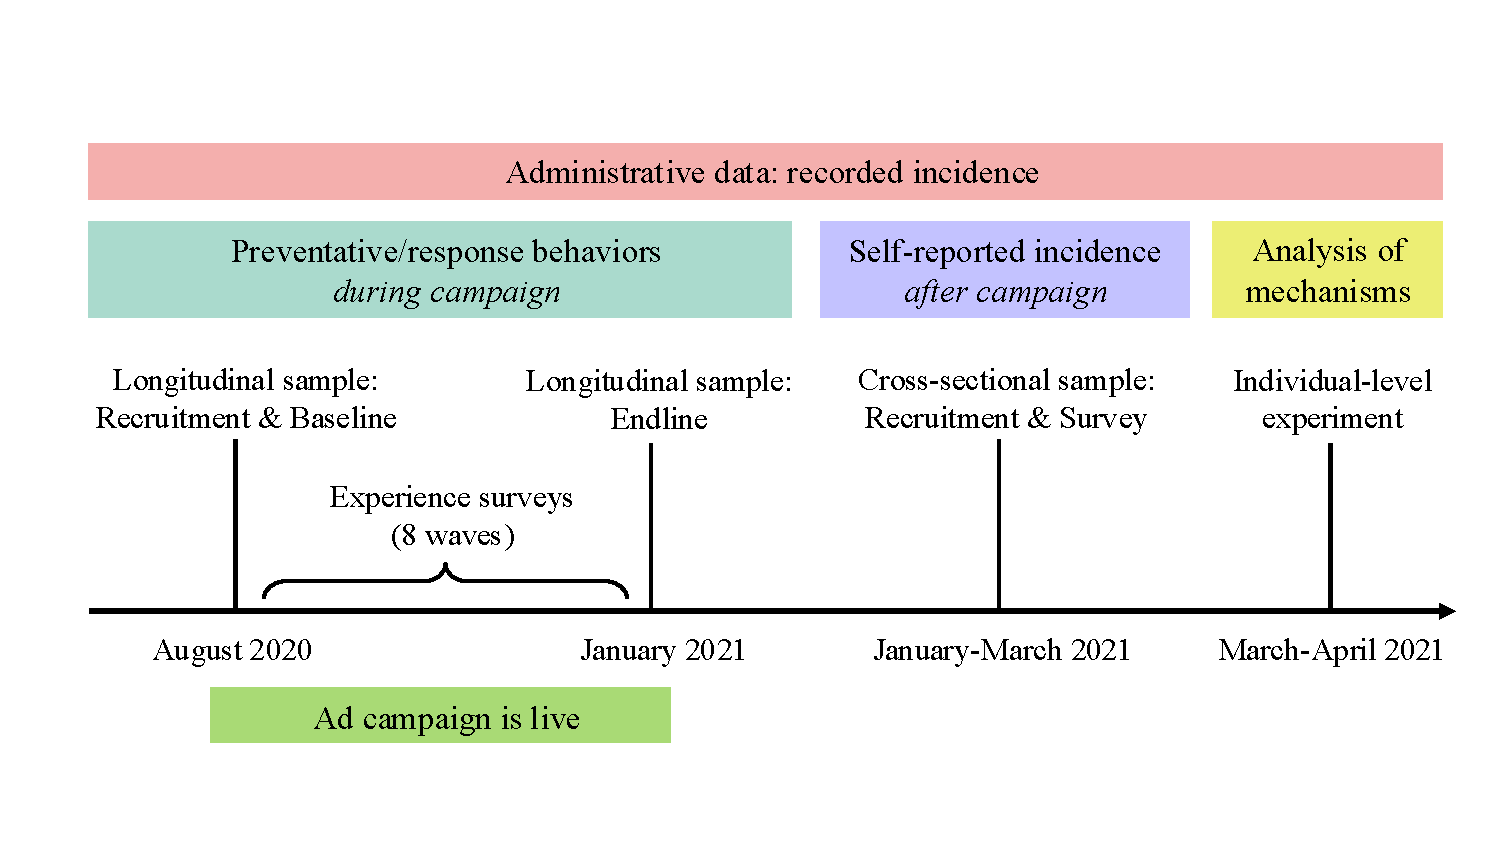
\includegraphics[scale=.58]{chapters/02-malaria/figures/Timeline.pdf}
    \label{fig:timeline}
\end{figure}


\subsection{Survey Samples and Administrative Data}\label{sec:data}

The longitudinal survey was designed to measure malaria-related preventive behaviors (such as bednet use) and response actions (such as seeking medical care when fever symptoms arise) during the campaign. It consisted of a baseline questionnaire fielded before or at the start of the campaign, an endline survey fielded near the end of the campaign and immediately afterward, and eight short intermediate surveys administered approximately every 17 days. All baseline respondents were invited to complete the endline, regardless of how many intermediate waves they completed. To study effects during the campaign, we restrict the analysis to responses collected between September 1, 2020 and January 31, 2021 and aggregate outcomes across waves at the individual level. The final longitudinal sample contains 5,201 individuals, evenly split between treatment and control districts.

The cross-sectional survey was designed to capture the accumulated and medium-term effects of the campaign on malaria incidence, risk perceptions, and bednet-related behaviors and intentions. Some questions from the longitudinal survey were repeated with longer recall windows. For example, whereas the longitudinal survey asked whether respondents or their family members had experienced malaria in the previous two weeks, the cross-sectional survey asked about malaria since August 2020, when the study campaign began. We also collected information on malaria risk perceptions and on intentions to purchase or retreat bednets with insecticide. The final cross-sectional sample contains 3,052 observations. As discussed in Section \ref{sec:mechanisms}, the cross-sectional study also served as the basis for an individual-level \textit{feed} experiment designed to distinguish between limited content effectiveness and limited campaign reach.

For both samples, recruitment was stratified by district and dwelling type, which we use as a practical proxy for variation in baseline socioeconomic conditions and malaria risk. The enrollment questionnaire asked participants about their preferred language (English, Hindi, or Odia) and provided information about the study before eliciting informed consent. Only respondents aged 18 or older who consented to participate were included in the survey samples. Prior to analysis, we cleaned the data to improve data integrity. Specifically, we excluded respondents who completed the survey unusually quickly, those older than 90, and those reporting households with more than 30 members. We also excluded observations with missing baseline covariates. Because some outcomes were not observed in every wave, respondents may still have missing dependent variables for particular outcomes or survey rounds; each analysis therefore uses all valid nonmissing responses available for the outcome under study. Table \ref{tab:data_cleaning} summarizes the data processing procedures.

\begin{table}[p]
\vspace{-2cm}
\centering
\footnotesize
\caption{Data sources, processing, and output}
\label{tab:data_cleaning}
\providecommand{\sym}[1]{\ifmmode^{#1}\else\(^{#1}\)\fi}
\begingroup
\renewcommand{\arraystretch}{0.94}
\hspace*{-1.7cm} 
\adjustbox{max width=\textwidth}{%
\begin{tabular}{p{3.6cm} p{6.8cm} p{6.8cm}}
\toprule
\textbf{\makecell[l]{Data (Source); \\ \textit{Level of Obs}}} & \textbf{Processing and cleaning procedures } & \textbf{Output} \\
\midrule

\makecell[l]{District Boundaries\\(Govt.);\\\emph{District}}
  & \makecell[l]{1) Remove 3 state capitals;\\ 2) Select 80 districts for study;\\ 3) Drop 1 due to attribution error\sym{*}}
  & \makecell[l]{79 study districts across 3 states} \\
\addlinespace \hline \addlinespace

\makecell[l]{Longitudinal Survey\\(Research team);\\\emph{Individual--wave}}
  & \makecell[l]{1) Responses Sep 1--Jan 31, with at \\ least one  nonmissing outcome:\\  \hspace{0.2cm} Obs=20,125, Ind.=6,954 \\
                 2) Drop quick responses\sym{**}:  \\ \hspace{0.2cm} Obs=15,940; Ind.=5,501 \\ 
                 3) Drop if age <18 or $\geq$90: \\ \hspace{0.2cm} Obs=15,307; Ind.=5,228 \\ 
                 4) Drop HHs $\geq$30 members:  \\ \hspace{0.2cm} Obs=15,259; Ind.=5,209 \\
                 5) Drop if missing covariates:  \\ \hspace{0.2cm} Obs=15,251; Ind.=5,201}
  & \makecell[l]{
Final sample at individual-wave level: 
15,251 obs \\ from 5,201 individuals in 79 study districts.\\
Nonmissing responses per outcome:\\
--Individual bednet use: Obs=15,250; Ind.=5,201 \\
--HH bednet use: Obs=14,792; Ind.=5,050 \\
--Long-sleeve clothing use: Obs=5,189; Ind.=5,174 \\
--Body/wall spray use: Obs=2,423; Ind.=2,351 \\
--Any fever in HH:  Obs=15,147; Ind.=5,158 \\
--Any malaria in HH: Obs=15,121; Ind.=5,141
}  \\
\addlinespace \hline \addlinespace

\makecell[l]{Cross‐sectional \\ Survey\\(Research team);\\\emph{Individual}}
  & \makecell[l]{1) Responses Jan 7--Mar 31,  \\ with nonmissing outcomes:  Ind.=3,368 \\
                 2) Drop quick responses\sym{**}: Ind.=3,060 \\
                 3) Drop if age <18 or $\geq$90: Ind.=3,060 \\
                 4) Drop HHs $\geq$30 members: Ind.=3,060 \\
                 5) Drop if missing covariates:  Ind.=3,052}
  & \makecell[l]{Final sample of 3,052 individuals  in 79 study \\ districts, with nonmissing malaria outcomes} \\
\addlinespace \hline \addlinespace

\makecell[l]{\textit{Feed} Experiment \\ Sample\\(Research team);\\\emph{Individual}}
  & \makecell[l]{1) Responses Mar 28--Apr 30, \\ with  nonmissing outcomes:  Ind.=1,565; \\
                 2) Drop quick responses\sym{**}: Ind.=1,545 \\
                 3) Drop if age <18 or $\geq$90: Ind.=1,545 \\
                 4) Drop HHs $\geq$30 members: Ind.=1,545 \\
                 5) Drop if missing covariates:  Ind.=1,542}
  & \makecell[l]{Final sample of 1,542 individuals  in 79 study \\ districts, with nonmissing bednet use and \\ treatment seeking outcomes} \\
\addlinespace \hline \addlinespace

\makecell[l]{Recorded Malaria \\Cases \\(HMIS, 2020-2021);\\\emph{Subdistrict-month}}
  & \makecell[l]{1) Apr 1,~2020--May 31,~2021;\\ 2) Drop unstable boundaries;\\ 3) Drop if N. cases>N. tests; \\ 4) Identify subdistrict population\\ overlapping with study circles}
  & \makecell[l]{395 subdistricts in 79 study districts;\\ 119 subdistricts with >50\%  population within \\study circles} \\
\addlinespace \hline \addlinespace

\makecell[l]{Census~2011 (Govt.);\\\emph{District}}
  & None
  & \makecell[l]{District-level covariates;\\ 121 districts, of which 79 selected in our study} \\
 \addlinespace \hline \addlinespace

\makecell[l]{DHS~2019--2021;\\\emph{Individual}}
  & \makecell[l]{Compute weighted means\\ by district}
  & \makecell[l]{District-level covariates;\\ 121 districts, of which 79 selected in our study}  \\
\addlinespace \hline \addlinespace

\makecell[l]{Population\\(UN WPP~2020);\\\emph{$1\,km \times 1\,km$}}
  & \makecell[l]{Compute district-level totals\\via GIS software}
  & \makecell[l]{Population counts control;\\ Rural vs. Urban pop. share;\\ 121 districts, of which 79 selected in our study} \\
\addlinespace \hline \addlinespace

\makecell[l]{Elevation (ETOPO5);\\\emph{$1\,km \times 1\,km$}}
  & \makecell[l]{Compute district-level means\\and st. dev. via GIS software}
  & \makecell[l]{Geographic controls;\\121 districts, of which 79 selected in our study} \\
\bottomrule

\multicolumn{3}{p{1.17\linewidth}}{\scriptsize \sym{*}One study district was excluded due to a data attribution issue during campaign implementation. Specifically, there were two districts named Balrampur---each in a different state. One of them was intended to be included in the study and assigned to the treatment group. Due to the same name, however,  it became impossible ex-post to determine which district was assigned to which condition. As a result, both were excluded from the analysis. \par \sym{**}We used timestamp data collected for each survey question to identify respondents who answered most questions unusually quickly. Specifically, we excluded respondents whose 90th percentile response time was less than three times their fastest response time. This approach accounts for individual variation in response speed while flagging uniformly fast response patterns suggestive of inattention and low engagement. }\\
\end{tabular}
}%

\endgroup

\end{table}

We complement the survey data with administrative health-facility records from the Indian Health Management Information System (HMIS), collected at the subdistrict-month level.\footnote{HMIS is a monitoring system established by the Indian Ministry of Health and Family Welfare (MoHFW). It collects facility-level monthly data on a wide range of health outcomes and aggregates them to the subdistrict, district, state, and national levels. The dataset is widely used in health research in India and is generally considered to satisfy standard thresholds for completeness and reliability \citep{sharma2016quality}.} The data report, for each subdistrict and month, the number of malaria tests conducted and the number of positive malaria cases recorded by health facilities. Because HMIS separately reports outcomes from urban and rural facilities within subdistricts, it allows us to estimate treatment effects by setting. Our analysis uses data from April 2020 to May 2021.\footnote{Although data are available for earlier periods, changes in subdistrict boundaries and in the number of subdistricts over time make consistent matching across years infeasible. We therefore restrict attention to the period over which administrative boundaries remain stable.} We define April to August 2020 as the pre-treatment period and September 2020 onward as the treatment period, consistent with the timing of campaign delivery in the study states. Relative to the survey data, the administrative records offer two main advantages. First, they provide objective measures of malaria incidence, mitigating concerns about social desirability bias or experimenter demand in self-reported outcomes. Second, they provide a broader measure of disease incidence at the subdistrict level, allowing us to estimate population-level effects of the campaign, including spillovers to individuals who were not directly exposed. They also allow for a more accurate assessment of the campaign’s cost-effectiveness.





\subsection{Outcome Measures}

We study three categories of outcomes: (1) self-reported protective behaviors and response actions during the campaign, (2) self-reported malaria incidence and related behaviors after the campaign, and (3) objectively recorded malaria outcomes from the Indian Health Management Information System (HMIS). Appendix \ref{mal-appendix:B} reports the underlying survey questions. 

\paragraph{Self-reported outcomes \textit{during} the campaign.}
The longitudinal survey repeatedly measured malaria-related protective behaviors and response actions over the course of the campaign. Using these repeated observations, we construct: (i) the share of survey waves in which the respondent reported using a bednet or other protective measures, (ii) the average share of household members who used a bednet, (iii) an indicator for whether any household member reported fever or malaria during the campaign period, and (iv) an indicator for whether the household engaged in timely care-seeking or malaria testing during the campaign period conditional on fever or malaria symptoms. These outcomes were measured approximately every 17 days, although not all questions were fielded in every wave. We therefore retain respondents who contribute at least one nonmissing observation for a given outcome. After cleaning, this yields 15,251 individual-wave observations from 5,201 respondents. For each outcome, we aggregate responses across waves using only valid nonmissing responses for that specific outcome: we use the mean for outcomes (i) and (ii), and the maximum for outcomes (iii) and (iv). In the pooled analysis, observations are weighted by the number of valid responses used to construct the corresponding respondent-level outcome. For robustness, we also report longitudinal specifications estimated at the individual-wave level. 

\paragraph{Self-reported outcomes \textit{after} the campaign.}
The cross-sectional survey measures accumulated and medium-term effects after the campaign ended. We ask whether any household member had malaria since August 2020, and, if so, how many household members were affected. We also elicit concerns about contracting malaria or COVID-19 in the following year. In addition, among bednet owners, we measure whether existing bednets were retreated with insecticide, while among non-owners we ask about willingness to purchase a bednet and knowledge of where to buy one. After cleaning, the cross-sectional sample contains 3,052 respondents. 




\paragraph{Health-facility recorded outcomes.}
We use HMIS records to construct objective measures of malaria incidence at the subdistrict-month level. For each subdistrict and month, we observe the number of malaria tests conducted, the number of positive malaria cases recorded by health facilities, and the relevant population counts. From these data, we construct malaria incidence rates, defined as recorded cases per million people, and test positivity rates, defined as positive cases per test conducted. Because HMIS separately reports outcomes for urban and rural health facilities within subdistricts, we can estimate effects separately by setting. We use malaria incidence and test positivity as our main objective health outcomes, and the number of tests conducted as a complementary measure of health-care utilization.




\subsection{Empirical Specifications}
\subsubsection{Analysis of Survey Data}

In the main survey specifications, the unit of observation is the individual. Respondents residing in districts where the campaign was delivered are assigned to the treatment group, while respondents in districts excluded from the campaign constitute the control group. Because respondents in treated districts were not necessarily exposed to the MNM ads, our survey estimates capture intent-to-treat (ITT) effects. Our baseline specification, estimated by Ordinary Least Squares, is
\begin{align} \label{eq:1}
y_{idz} = \alpha + \beta T_{dz} + \theta_z + \epsilon_{idz},
\end{align}
where $i$ indexes individuals, $d$ districts, and $z$ states. $T_{dz}$ is an indicator equal to one if district $d$ in state $z$ was assigned to treatment. The coefficient of interest, $\beta$, captures the causal effect of assignment to the campaign on outcome $y$. For binary outcomes, equation (\ref{eq:1}) is estimated as a linear probability model. All specifications include state fixed effects, $\theta_z$, and standard errors clustered at the district level to allow for arbitrary within-district correlation in $\epsilon_{idz}$.

Because treatment was randomly assigned and baseline characteristics are well balanced across treatment and control districts, this parsimonious specification identifies causal effects without requiring additional controls. As robustness checks, we assess the sensitivity of the results to the inclusion of covariates and to alternative estimators. In particular, for binary outcomes we also estimate logistic models and report marginal effects. For outcomes observed repeatedly during the campaign, we additionally report longitudinal specifications at the individual-wave level with wave fixed effects.



\subsubsection{Analysis of Administrative Data}

Administrative data were collected at the subdistrict level and cover 395 subdistricts across the 79 districts in the analysis. Focusing on subdistricts, rather than entire districts, reduces measurement error and improves precision by allowing a closer alignment between the data and the treatment and control areas, which were defined using circular zones within districts (Figure \ref{fig:clusters}). This helps mitigate concerns that district-level health-facility records in control districts may partly reflect outcomes for individuals exposed to the campaign.\footnote{Our cluster-level design was based on circles around major cities rather than district boundaries (Section \ref{sec:cluster-design}). In control districts, some areas were excluded from the campaign using these circles. While survey respondents were sampled from within the circles, district-level administrative records could still capture outcomes from exposed individuals, potentially biasing estimates toward zero. Subdistrict-level data reduce this concern by allowing a closer alignment with the defined circles.} Using GIS tools, we identified the areas of overlap between subdistricts and study circles and computed the share of each subdistrict’s population living within those overlapping areas. We then used this measure to define alternative subsamples of subdistricts: the higher the overlap share, the lower the potential contamination in the control group.

Our benchmark specification focuses on the 119 subdistricts with at least 50\% of their population living within the study circles. We also report the sensitivity of the results to alternative overlap thresholds, ranging from 10\% to 80\%.\footnote{A sufficiently large sample is needed to retain adequate statistical power. Thresholds above 80\% leave too few observations for reliable inference.} Table \ref{tab:dd_sample} reports the mean monthly outcomes for the full set of subdistricts and for the benchmark subsample. While the number of malaria cases per month is similar across the two samples, monthly incidence per million people is substantially lower in the benchmark subsample (about 21 versus 51 cases per million), reflecting the larger average population of the subdistricts covered by the study circles, which were centered on major towns and cities. The table also reports means separately for urban and rural health facilities.\footnote{Not all subdistricts contain both types of facilities. Among the 119 subdistricts in the benchmark sample, 116 have rural health facilities and 65 have urban health facilities.} These figures highlight the greater burden of malaria in rural areas. For example, in the benchmark sample, both absolute incidence and incidence per million are roughly twice as large in rural facilities (9 cases and 19 cases per million) as in urban facilities (4.8 cases and 9.5 cases per million). %To improve data integrity, we exclude subdistrict-month observations in which the number of positive malaria cases exceeds the number of malaria tests conducted.

\begin{table}[!htbp]
    \centering
    \caption{Administrative health-facility data: mean monthly outcomes across subdistricts}
    \footnotesize
    \hspace*{-1.5cm}
    {
\def\sym#1{\ifmmode^{#1}\else\(^{#1}\)\fi}
\adjustbox{max width=\textwidth}{%
\begin{tabular}{l*{6}{c}}
\hline\hline
                    &\multicolumn{3}{c}{All subdistricts}  &\multicolumn{3}{c}{Subdistricts with >50\% population within circles}\\\cmidrule(lr){2-4}\cmidrule(lr){5-7}
                    &All health facilities&       Urban&       Rural&All health facilities&       Urban&       Rural\\
\hline
N. of cases         &        9.63&        3.65&        9.37&       10.05&        4.76&        8.93\\
N. of cases per M people&       51.23&        7.33&       53.80&       20.89&        9.45&       18.87\\
N. of tests per M people&     3278.63&     1050.34&     3267.20&     2689.72&     1221.98&     2425.33\\
Test positivity rate (\%)&        1.50&        1.45&        1.43&        1.24&        1.71&        1.10\\
Population (Thousand)&      550.35&      905.92&      509.51&      716.82&      960.55&      656.96\\
\hline
N. of subdistricts  &   \num{395}&   \num{111}&   \num{392}&   \num{119}&    \num{65}&   \num{116}\\
\hline\hline
\multicolumn{7}{p{1.10\linewidth}}{\scriptsize  Notes: The table reports the means of the variables across the different subsamples. Only subdistricts with non-missing entries are included. Subdistricts where the number of positive malaria cases was larger than the number of malaria tests conducted are dropped. Subdistricts often include both urban and rural areas. As a result, malaria incidence is reported separately for urban and rural health facilities within the same subdistrict, and the corresponding sample sizes do not necessarily sum to the total number of subdistricts. }\\
\end{tabular}
}%

}

    \label{tab:dd_sample}
\end{table}

To estimate the effect of the campaign, we exploit within-subdistrict variation between April 2020 and May 2021 and estimate the following Difference-in-Differences specification:
\begin{align} \label{eq:3}
y_{sdt} = \alpha + \beta \, T_{d} \times \text{Post}_{t} + \gamma \, \mathbf{x}_{sd} \times \text{Post}_{t} + \delta \, \mathbf{w}_{d} \times \text{Post}_{t} + \mu_{s} + \psi_{t} + \epsilon_{sdt},
\end{align}
where $y_{sdt}$ is the outcome for subdistrict $s$ in district $d$ and month $t$. $T_d$ is an indicator equal to one if district $d$ was assigned to treatment, and $\text{Post}_t$ is an indicator equal to one from September 2020 onward, after the campaign began. The specification includes subdistrict fixed effects, $\mu_s$, and month-by-year fixed effects, $\psi_t$, to absorb time-invariant differences across subdistricts and common seasonality in malaria outcomes. In all regressions, we also include state fixed effects interacted with $\text{Post}_t$. Depending on the specification, we further include pre-treatment district- and subdistrict-level controls, $\mathbf{w}_d$ and $\mathbf{x}_{sd}$, interacted with $\text{Post}_t$, to account for factors that may differentially affect outcomes over time. Standard errors are clustered at the district level to allow for both serial and cross-sectional correlation within districts. The coefficient of interest, $\beta$, captures the causal effect of the campaign under the identifying assumption of parallel trends, namely that in the absence of treatment, malaria outcomes in treatment and control subdistricts would have evolved similarly over time. Although random assignment of the campaign makes this assumption more plausible, we also provide empirical evidence consistent with it.


\section{Results}

\subsection{Sample Characteristics and Randomization Checks}

Annex Tables \ref{tab:panel_sample_balance} and \ref{tab:cross_section_balance} in the Appendix describe the characteristics of individuals and households in the longitudinal and cross-sectional samples, respectively. The tables report variable means in the treatment and control groups, normalized differences, and the corresponding \textit{p}-values from tests of equality. For the longitudinal sample, we report both covariates (Panel A) and baseline outcomes (Panel B). For the cross-sectional sample, which was collected after the campaign, we report only time-invariant covariates.

Both tables indicate a high degree of balance in individual and household characteristics, as well as in pre-treatment outcomes, across experimental groups, supporting the validity of the randomization. In the longitudinal sample, none of the differences between treatment and control groups is statistically significant. Annex Table \ref{tab:panel_sample_balance_attrition} shows that this balance is preserved after accounting for attrition. In the cross-sectional sample, the treatment group includes a slightly higher proportion of unemployed individuals and households with pregnant women than the control group. However, these differences are small in magnitude, with all normalized differences below 0.07. In addition, our main results are robust to the inclusion of control variables.

In both samples, respondents are roughly evenly split between treatment and control districts, and approximately 55\% reside in non- or semi-solid dwellings, consistent with the stratified recruitment design across districts and dwelling type. Attrition in the longitudinal sample is also balanced across experimental groups, with respondents completing, on average, three survey waves. Annex Table \ref{tab:panel_attrition_by_arm} further reports results from a survey-wave differential attrition test, showing that nonresponse rates were balanced across treatment and control arms. In terms of socio-demographic characteristics, men make up about 90\% of both samples, the average respondent is 27 years old, and 55\% to 60\% report having completed university, while about half are unemployed. Around 60\% of respondents identify with socially and economically disadvantaged caste groups (OBC, SC/Dalit, and ST), which prior studies suggest are associated with lower awareness of malaria prevention \citep{malaria_SES_2020}. Household size ranges from 6 to 7 members on average. About one in eight households includes a pregnant woman, and roughly three-quarters of respondents live within 60 minutes’ walking distance of a medical center.

In terms of baseline outcomes, 2\% of respondents report that a household member experienced malaria in the previous two weeks, and 20\% report a malaria episode within the previous five years. Among households that own a bednet, about 70\% report that the respondent slept under it the previous night, and about 70\% report that household members did so as well. Combining these figures with the average bednet ownership rate in the sample (75\%) implies that just over half of individuals are regularly protected from mosquito bites at night. Relatedly, about one-third of respondents report some concern about getting malaria in the following month.

Relative to the general population, our sample of social media users is socioeconomically more advantaged, based on data from the 2019--2021 India Demographic and Health Survey \citep{dhs2022}. While approximately three-quarters of households in our sample own a mosquito net, only about one-third of households in India report owning at least one. Internet access is also more limited in the broader population: across the three study states, only about one in three women and six in ten men have ever used the internet. These differences imply that our findings apply to connected populations and do not generalize to individuals without internet access.

Finally, for the analysis based on health-facility data, we examine balance on pre-treatment characteristics at the subdistrict level. Annex Table \ref{tab:subdistricts_balance} shows that treatment and control subdistricts are generally balanced on observed characteristics such as population, the rural population share, and geographic indicators. For malaria-related outcomes---including the number of diagnostic tests and test positivity rates---there are no statistically significant differences across experimental conditions. Although both urban and rural positivity rates are slightly higher in treatment areas, these differences are small in standard deviation units and not statistically significant. Moreover, the Difference-in-Differences specification further mitigates concerns about residual pre-campaign imbalances by including subdistrict fixed effects.

\subsection{Survey-based Results} \label{sec:servey_results}

\subsubsection{Protective behaviors, care-seeking, and health outcomes during the campaign}
Table \ref{tab:bednets_ols} presents the effect of the campaign on sleeping under mosquito nets during the intervention period---one of the main behaviors emphasized in the ads that received the largest share of the budget. We report results for both respondents’ own behavior and that of the entire household. The analysis focuses on households that owned at least one bednet at baseline, allowing us to isolate changes in usage behavior rather than conflating them with ownership decisions.\footnote{The campaign did not explicitly promote bednet purchases, and we find no effect on bednet ownership.}  For each outcome, we report results using two alternative specifications. Columns (1) and (3) present pooled individual-level estimates, where outcomes are aggregated across survey waves and weighted by the number of completed waves. Columns (2) and (4) report longitudinal estimates at the individual–wave level, including wave fixed effects. 

Across all specifications, the estimated effects are small and not statistically significant. The point estimates correspond to increases of about 3 percentage points (p.p.) at the individual level and about 2.5 p.p. at the household level (approximately 4–5\% relative to the control mean), but we cannot reject the null of no effect. The similarity of the estimates across specifications indicates that the results are robust to the level of aggregation and to the inclusion of within-individual variation over time.

\begin{table}[h!]
    \centering
    \caption{Sleeping under bednet (during the campaign)}
    \footnotesize
    %\hspace*{-0.6cm}
    {
\def\sym#1{\ifmmode^{#1}\else\(^{#1}\)\fi}
\adjustbox{max width=\textwidth}{%
\begin{tabular}{l*{4}{c}}
\hline\hline
                &\multicolumn{2}{c}{Share of times respondent used bednet}&\multicolumn{2}{c}{Share of HH members who used bednet}\\\cmidrule(lr){2-3}\cmidrule(lr){4-5}
                &\multicolumn{1}{c}{(1)}         &\multicolumn{1}{c}{(2)}         &\multicolumn{1}{c}{(3)}         &\multicolumn{1}{c}{(4)}         \\
Unit of analysis:                &   Individual         &Individual-wave        &   Individual         &Individual-wave        \\
\hline
T               &    0.030         &    0.030         &    0.025         &    0.025         \\
                &  (0.019)         &  (0.019)         &  (0.017)         &  (0.018)         \\
Wave FE         &                  &$\checkmark$         &                  &$\checkmark$         \\
\hline
Observations    &\num{4004}         &\num{11965}         &\num{3900}         &\num{11619}         \\
Adj. R-squared  &    0.006         &    0.007         &    0.005         &    0.006         \\
Mean in control &    0.635         &    0.635         &    0.661         &    0.661         \\
SD in control   &    0.421         &    0.481         &    0.344         &    0.380         \\
\hline\hline
\multicolumn{5}{p{0.9\linewidth}}{\scriptsize Notes: The table reports intent-to-treat estimates of the campaign’s effect on bednet use during the campaign period, using responses collected between September 1, 2020 and January 31, 2021. Only households owning at least one bednet are included. \(T\) is the treatment indicator. Columns (1) and (3) report pooled individual-level specifications in which the outcome is the share of survey waves with reported bednet use and observations are weighted by the number of valid survey responses, while columns (2) and (4) report longitudinal (panel) specifications at the individual--wave level with wave fixed effects. State fixed effects are included in all columns. Standard errors are clustered at the district level. \sym{*} \(p<0.1\), \sym{**} \(p<0.05\), \sym{***} \(p<0.01\)}\\
\end{tabular}
}%

}

    \label{tab:bednets_ols}
\end{table}

\begin{figure}[h!]
    \centering
    \caption{Effects on household-level bednet use by survey month and malaria concern levels}
    \begin{minipage}{16cm}
    \hspace{-1.3cm}
    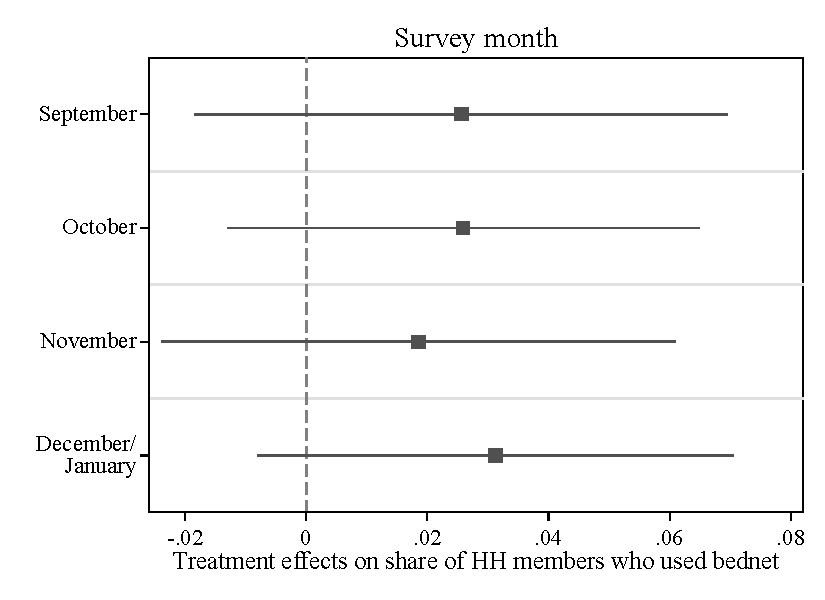
\includegraphics[scale=0.65]{chapters/02-malaria/figures/bednets_ols_bymonth.pdf}
     \hspace{-.4cm}
    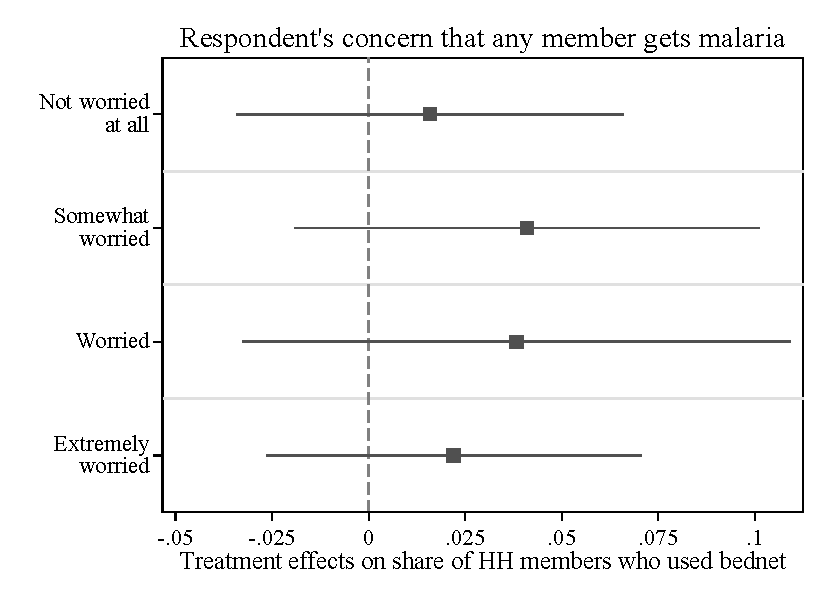
\includegraphics[scale=0.65]{chapters/02-malaria/figures/bednets_ols_byworried.pdf}
    \label{fig:bednets_ols_byworried}
    \end{minipage}
    \begin{minipage}{16.5cm}
    \vspace{-0.5cm}
\scriptsize{Notes: The figure reports coefficient estimates (treatment effects) from the regression in column (3) of Table \ref{tab:bednets_ols}, estimated separately for different sub-samples defined by the month in which the survey was taken (left panel) and by baseline malaria concern (right panel). The outcome is the share of household members who used a bednet the previous night. The sample is restricted to households that owned at least one bednet at baseline. Bars indicate 95\% confidence intervals. All regressions include state fixed effects, and standard errors are clustered at the district level.}
\end{minipage}
\end{figure}

Figure \ref{fig:bednets_ols_byworried} examines heterogeneity in the treatment effects of the campaign on household-level bednet use across different periods of the campaign (left panel) and across baseline risk perception levels (right panel). A natural question is whether estimated effects differ over the course of the campaign and across households with different baseline levels of concern about malaria. However, consistent with the small and statistically insignificant estimates reported in Table \ref{tab:bednets_ols}, we find no evidence of heterogeneous effects along either dimension.




\begin{table}[h!]
    \centering
    \caption{Other protective behaviors (during the campaign)}
    \footnotesize
    %\hspace*{-1cm}
    {
\def\sym#1{\ifmmode^{#1}\else\(^{#1}\)\fi}
\adjustbox{max width=\textwidth}{%
\begin{tabular}{l*{3}{c}}
\hline\hline
                &\multicolumn{1}{c}{\shortstack{Share of times any member\\used long sleeves}}&\multicolumn{1}{c}{\shortstack{Share of times any member\\used body/wall sprays}}&\multicolumn{1}{c}{\shortstack{Protective Behaviors\\ Index}}\\\cmidrule(lr){2-2}\cmidrule(lr){3-3}\cmidrule(lr){4-4}
                &      (1)         &      (2)         &      (3)         \\
\hline
T               &   -0.005         &   -0.020         &    0.004         \\
                &  (0.019)         &  (0.023)         &  (0.049)         \\
\hline
Observations    &\num{5174}         &\num{2351}         &\num{5201}         \\
Adj. R-squared  &    0.014         &    0.002         &    0.002         \\
Mean in control &    0.642         &    0.410         &    0.069         \\
SD in control   &    0.404         &    0.485         &    0.937         \\
\hline\hline
\multicolumn{4}{p{0.9\linewidth}}{\scriptsize Notes: The table reports intent-to-treat estimates of the campaign’s effect on alternative protective behaviors during the campaign period, using responses collected from September 1, 2020 to January 31, 2021. Each observation is an individual and observations are weighted by the number of survey waves the respondent completed in this period. \(T\) is the treatment indicator. Columns (1) and (2) report the share survey waves with reported use of long-sleeved clothing and mosquito sprays, respectively, by any household member. Column (3) reports a standardized protective behaviors index constructed using Principal Component Analysis applied to individual bednet use, the share of household members using bednets, and individual use of mosquito spray and long-sleeved clothing. Since some components are missing for a subset of observations, missing values are imputed at the sample mean in constructing the index.  Standard errors are clustered at the district level. \sym{*} \(p<0.1\), \sym{**} \(p<0.05\), \sym{***} \(p<0.01\).}\\
\end{tabular}
}%

}

    \label{tab:protective_index_ols}
\end{table}


We also examine the effects of the MNM campaign on other protective behaviors, such as wearing long-sleeved clothing and using body or wall sprays to prevent mosquito bites. Table \ref{tab:protective_index_ols} shows no statistically significant effects on these behaviors. The estimated coefficients are small and, if anything, negative. Column (3) reports results for a composite protective-behavior index constructed using principal component analysis of bednet use, the share of household members using bednets, and the use of sprays and long-sleeved clothing. Unlike the bednet-use analysis, this index is constructed for the full sample rather than only for bednet owners. Consistent with the individual outcomes, we find no significant effect of the campaign on this composite measure.

Our results provide no clear evidence that the campaign significantly affected either its primary behavioral target---bednet use---or other related protective behaviors. This lack of detectable effects may reflect either limited effectiveness of the ads in changing behavior or insufficient exposure among the relevant population, a distinction we explore in Section \ref{sec:mechanisms}.


\begin{table}[h!]
    \centering
    \caption{Incidence of fever, care-seeking, and malaria outcomes  (during the campaign)}
    \footnotesize
    %\hspace*{-0.6cm}
    {
\def\sym#1{\ifmmode^{#1}\else\(^{#1}\)\fi}
\adjustbox{max width=\textwidth}{%
\begin{tabular}{l*{8}{c}}
\hline\hline
                &\multicolumn{2}{c}{Any fever}        &\multicolumn{2}{c}{Care-seeking (24h)}&\multicolumn{2}{c}{Any malaria}      &\multicolumn{2}{c}{Malaria test}     \\\cmidrule(lr){2-3}\cmidrule(lr){4-5}\cmidrule(lr){6-7}\cmidrule(lr){8-9}
                &\multicolumn{1}{c}{(1)}         &\multicolumn{1}{c}{(2)}         &\multicolumn{1}{c}{(3)}         &\multicolumn{1}{c}{(4)}         &\multicolumn{1}{c}{(5)}         &\multicolumn{1}{c}{(6)}         &\multicolumn{1}{c}{(7)}         &\multicolumn{1}{c}{(8)}         \\
                &      OLS         &    Logit         &      OLS         &    Logit         &      OLS         &    Logit         &      OLS         &    Logit         \\
\hline
T               &    0.007         &    0.045         &    0.006         &    0.044         &   -0.004         &   -0.061         &    0.003         &    0.017         \\
                &  (0.017)         &  (0.102)         &  (0.030)         &  (0.211)         &  (0.010)         &  (0.146)         &  (0.061)         &  (0.294)         \\
\hline
Observations    &\num{5158}         &\num{5158}         &\num{724}         &\num{724}         &\num{5141}         &\num{5141}         &\num{324}         &\num{324}         \\
Adj. R-squared  &    0.002         &                  &   -0.000         &                  &    0.003         &                  &   -0.008         &                  \\
Pseudo R-squared&                  &    0.003         &                  &    0.004         &                  &    0.008         &                  &    0.001         \\
Marginal effect &                  &    0.007         &                  &    0.006         &                  &   -0.004         &                  &    0.003         \\
Mean in control &    0.202         &    0.156         &    0.824         &    0.797         &    0.062         &    0.062         &    0.679         &    0.679         \\
SD in control   &    0.402         &    0.363         &    0.381         &    0.403         &    0.241         &    0.241         &    0.468         &    0.468         \\
\hline\hline
\multicolumn{9}{p{.9\linewidth}}{\scriptsize  Notes: The table reports intent-to-treat estimates of the campaign’s effect on fever, care-seeking, and malaria-related outcomes during the campaign period, using responses collected from September 1, 2020 to January 31, 2021. Each observation is an individual, and observations are weighted by the number of survey waves the individual completed in this period. \(T\) is the treatment indicator. Columns (1) and (2) report indicators for whether any household member experienced a high fever (100.4°F / 38°C or above) at least once during the period; columns (3) and (4) report indicators for whether any household member with fever sought medical help within 24 hours at least once. Columns (5) and (6) report indicators for whether any household member had malaria at least once during the period; and columns (7) and (8) report indicators for whether any household member with malaria was tested at least once.  State fixed effects are included in all columns.  Standard errors are clustered at the district level. \sym{*} \(p<0.1\), \sym{**} \(p<0.05\), \sym{***} \(p<0.01\).}\\
\end{tabular}
}%

}

    \label{tab:fever_panel_ols}
\end{table}

We next examine malaria-related health outcomes and response actions during the campaign. In the longitudinal sample, respondents were repeatedly asked whether anyone in the household had experienced fever (100.4$^\circ$F / 38$^\circ$C or above) or malaria in the previous two weeks. Conditional on fever, we measure whether medical help was sought within 24 hours; conditional on malaria, we measure whether the individual was tested. Timely care-seeking and malaria testing were both emphasized in the campaign. Table \ref{tab:fever_panel_ols} reports the effects of the campaign on these outcomes, defined as indicators equal to one if the event occurred at least once during the campaign period.

Across all outcomes, the estimated effects are small and not statistically significant. We do not detect changes in the incidence of fever or malaria (columns 1--2 and 5--6), nor in timely care-seeking or malaria testing conditional on symptoms (columns 3--4 and 7--8). The results are similar across OLS and logit specifications, with marginal effects from the latter closely matching the OLS estimates. Taken together, these findings provide no evidence of detectable effects on malaria-related health outcomes or response actions during the intervention period. This may reflect the fact that any behavioral responses induced by the campaign were too limited or too short-lived to translate into measurable health effects during the campaign itself. These considerations motivate our analysis of post-campaign outcomes using the separate cross-sectional sample and the administrative data.





\subsubsection{Malaria incidence and bednet re-treatment after the campaign}

Table \ref{tab:malaria_xsection_ols} presents the impact of the campaign on self-reported malaria incidence since its launch in August 2020, as measured in the cross-sectional survey conducted 1–3 months after the campaign ended. The table reports outcomes at both the extensive margin (whether any household member had malaria; columns 1–2) and the intensive margin (the share of household members infected; column 3). Across all measures, we find no statistically significant impact of the campaign on malaria incidence. The estimated effects are small and close to zero, and we cannot reject the null of no effect. Results are consistent across OLS and logit specifications.

Figure \ref{fig:share_malaria_bynet} examines whether the effects of the campaign vary with bednet ownership and coverage. The left panel compares households with and without bednets, while the right panel focuses on households with bednets and distinguishes between those with higher and lower coverage (measured as at least one bednet for every two members). Across all subgroups, the estimated effects are small and not statistically significant. Overall, the figure provides no evidence that bednet ownership or coverage moderates the impact of the campaign on malaria outcomes.

Columns (4) and (5) of Table \ref{tab:malaria_xsection_ols} examine whether respondents re-treated their bednets with insecticide. In contrast to the incidence results, the retreatment estimates are positive and marginally statistically significant. The OLS estimate corresponds to a 5.1 p.p. increase among bednet owners. While this points to some behavioral response along this margin, the estimate remains imprecise.

%Overall, the absence of detectable effects on malaria incidence is consistent with the null results observed for protective behaviors during the campaign.




\begin{table}[h!]
    \centering
    \caption{Malaria incidence and bednet re-treatment with insecticide (since campaign launch)}
    \footnotesize
    \hspace*{-0.2cm}
    {
\def\sym#1{\ifmmode^{#1}\else\(^{#1}\)\fi}
\adjustbox{max width=\textwidth}{%
\begin{tabular}{l
    >{\centering\arraybackslash}p{1.7cm}
    >{\centering\arraybackslash}p{1.7cm}
    >{\centering\arraybackslash}p{3.4cm}
    >{\centering\arraybackslash}p{1.7cm}
    >{\centering\arraybackslash}p{1.7cm}}
\hline\hline
                &\multicolumn{2}{c}{\shortstack{Any HH member\\had malaria}}&\multicolumn{1}{c}{\shortstack{Share of HH members\\who had malaria}}&\multicolumn{2}{c}{\shortstack{Any bednet retreated\\with insecticide}}\\\cmidrule(lr){2-3}\cmidrule(lr){4-4}\cmidrule(lr){5-6}
                &\multicolumn{1}{c}{(1)}         &\multicolumn{1}{c}{(2)}         &\multicolumn{1}{c}{(3)}         &\multicolumn{1}{c}{(4)}         &\multicolumn{1}{c}{(5)}         \\
                &      OLS         &    Logit         &      OLS         &      OLS         &    Logit         \\
\hline
T               &    0.003         &    0.053         &   -0.002         &    0.051\sym{*}  &    0.207\sym{*}  \\
                &  (0.011)         &  (0.196)         &  (0.003)         &  (0.027)         &  (0.108)         \\
\hline
Observations    &\num{3052}         &\num{3052}         &\num{3052}         &\num{2017}         &\num{2017}         \\
Adj. R-squared  &   -0.000         &                  &    0.001         &    0.001         &                  \\
Pseudo R-squared&                  &    0.001         &                  &                  &    0.002         \\
Marginal effect &                  &    0.003         &                  &                  &    0.051         \\
Mean in control &    0.058         &    0.058         &    0.016         &    0.409         &    0.409         \\
SD in control   &    0.235         &    0.235         &    0.081         &    0.492         &    0.492         \\
\hline\hline
\multicolumn{6}{p{.9\linewidth}}{\scriptsize Notes: Each observation is an individual. \(T\) is the treatment indicator. All responses were collected after the campaign, between January 7 and March 31, 2021. Columns (1) and (2) report indicators for whether any household member had malaria since August 2020. Column (3) reports the share of household members with malaria since August 2020. Columns (4) and (5) report whether the respondent retreated their bednet (conditional on having at least one) with insecticide since August 2020. State fixed effects are included in all columns. Standard errors are clustered at the district level. \sym{*} \(p<0.1\), \sym{**} \(p<0.05\), \sym{***} \(p<0.01\).}\\
\end{tabular}
}%

}

    \label{tab:malaria_xsection_ols}
\end{table}


\begin{figure}[h!]
    \centering
    \caption{Effects on household-level malaria incidence by bednet ownership and coverage}
\begin{minipage}{20cm}
   \hspace{-1.3cm}
    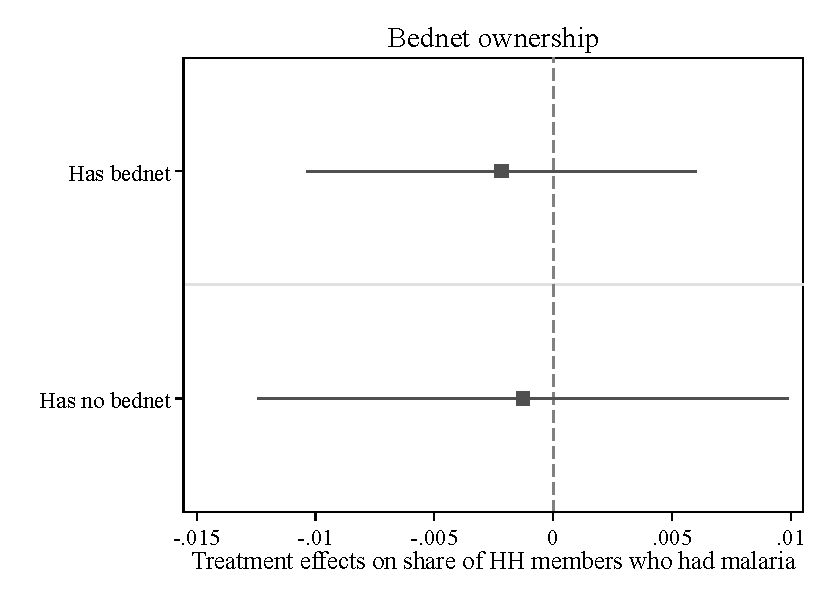
\includegraphics[scale=0.65]{chapters/02-malaria/figures/share_malaria_bynet.pdf}
    \hspace{-.25cm}
    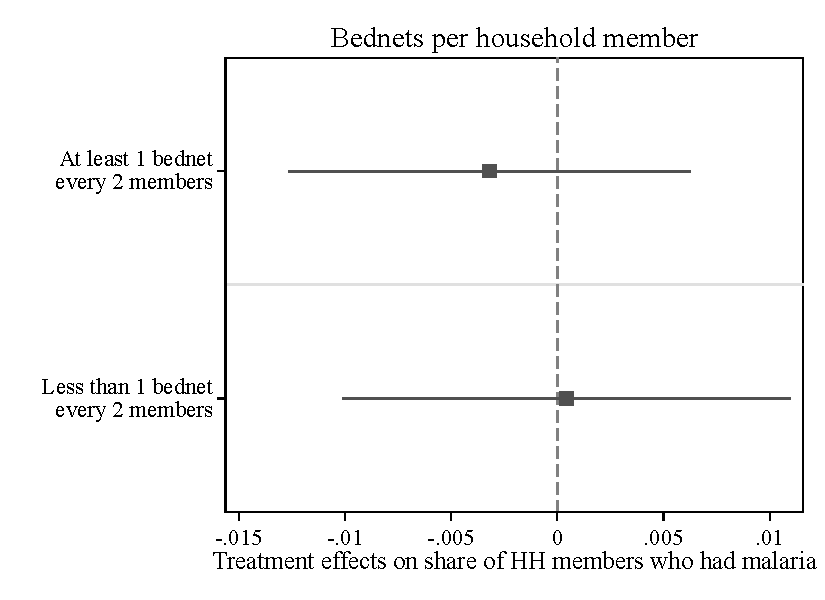
\includegraphics[scale=0.65]{chapters/02-malaria/figures/share_malaria_bynumnet.pdf}
    \label{fig:share_malaria_bynet}
\end{minipage}
   \begin{minipage}{16.5cm}
\scriptsize{Notes: The figure reports coefficient estimates (treatment effects) from the regression in column (3) of Table \ref{tab:malaria_xsection_ols}, estimated separately for different sub-samples defined by household bednet ownership (left panel) and by the number of bednets per household member (right panel). The outcome is the share of household members who had malaria since August 2020. Bars indicate 95\% confidence intervals. Standard errors are clustered at the district level.}
\end{minipage}
\label{tab:share_malaria_bynet}
\end{figure}



Finally, Annex Table \ref{tab:treat_buy_net_xsection_ols} assesses whether the campaign affected malaria-related concern and bednet-related intentions after the campaign ended. We find only marginally significant evidence ($p<0.1$) that the campaign increased the share of respondents who report being very worried about malaria in the following year, with an estimated effect of 2.9 p.p., or about 11\% relative to the control mean (columns 1–2). By contrast, we find no significant effects on bednet ownership, willingness to buy a bednet among non-owners, or knowledge of where to buy one (columns 3–8).\footnote{This pattern is also consistent with the content of the campaign, which did not explicitly seek to promote bednet purchases.} Taken together, these results suggest that the campaign may have modestly increased concern about malaria, without translating into stronger bednet-related adoption or purchase intentions.



\subsubsection{Heterogeneous treatment effects by Household Socio-Economic Status}

We next explore, in a post-hoc and exploratory manner, whether the campaign’s effects varied across households with different levels of socioeconomic status (SES). We use SES as a pre-treatment moderator in this analysis: the estimates describe heterogeneity in the randomized treatment effect across SES groups, rather than isolating any single underlying channel. The index combines housing choice, proximity to health facilities, education, caste status, air-conditioning ownership, and household size, and may also capture unobserved factors that shape social-media use, digital engagement, and the ability to respond to health messages. Focusing on this index is useful because Table~\ref{tab:malaria_correlates} shows that its components are jointly informative about baseline malaria incidence and reports the loadings of the first principal component used to construct it. Higher SES is associated with more protective living conditions: for example, solid housing and closer access to health facilities load positively into the index, whereas larger household size loads negatively.

Annex Table~\ref{tab:malaria_predictors} further shows that the SES index is negatively associated with malaria incidence at baseline. A one-standard-deviation increase in SES is associated with a 2.2 p.p. lower probability that any household member had malaria in the previous five years and a 0.4 p.p. lower probability of malaria in the previous two weeks. Relative to the corresponding sample means, these associations amount to reductions of about 12\% and 25\%, respectively. Motivated by this relationship, we use the SES index to examine whether the campaign had differential effects across households with relatively lower and higher socioeconomic status, and thus across groups that were ex ante more and less vulnerable to malaria risk.

To do so, we focus on the main behavioral and health outcomes discussed above and split the sample at the median of the standardized first principal component into higher- and lower-SES households. We then estimate treatment effects separately by SES group and test for differences using a pooled regression that includes the treatment indicator, a high-SES indicator, and their interaction, $T \times \text{HighSES}$. The interaction coefficient captures whether the treatment effect differs across the SES distribution. We report both conventional \textit{p}-values and \textit{p}-values adjusted for multiple testing using the Benjamini--Hochberg false discovery rate (FDR) procedure \citep{benjamini1995controlling}.

\begin{table}[t]
    \centering
    \caption{Treatment effect heterogeneity by Household Socio-Economic Status (SES)} 
     \footnotesize
    {
\def\sym#1{\ifmmode^{#1}\else\(^{#1}\)\fi}
\adjustbox{max width=\textwidth}{%
\begin{tabular}{l
    >{\centering\arraybackslash}p{2.2cm}
    >{\centering\arraybackslash}p{2.2cm}
    >{\centering\arraybackslash}p{2.2cm}
    >{\centering\arraybackslash}p{2.2cm}}
\hline\hline \vspace{-0.3cm} \\
                &\multicolumn{2}{c}{\shortstack{Share of HH members \\ who   used bednet}}&\multicolumn{2}{c}{\shortstack{Any HH member had a fever  \\ during  the campaign}}\\\cmidrule(lr){2-3}\cmidrule(lr){4-5}
                &\multicolumn{1}{c}{(1)}         &\multicolumn{1}{c}{(2)}         &\multicolumn{1}{c}{(3)}         &\multicolumn{1}{c}{(4)}         \\
                & High SES         &  Low SES         & High SES         &  Low SES         \\
\hline 
T               &    0.067\sym{***}&   -0.016         &    0.003         &    0.011         \\
                &  (0.024)         &  (0.019)         &  (0.020)         &  (0.022)         \\
\hline
T p-value (FDR) &\num{0.048}         &\num{0.651}         &\num{0.866}         &\num{0.689}         \\
\emph{T}$\times$\emph{High SES} coef.
                & \multicolumn{2}{c}{\num{0.084}}
                & \multicolumn{2}{c}{\num{-0.006}} \\

\emph{T}$\times$\emph{High SES} p-value
                & \multicolumn{2}{c}{\num{0.001}}
                & \multicolumn{2}{c}{\num{0.820}} \\

\emph{T}$\times$\emph{High SES} p-value (FDR)
                & \multicolumn{2}{c}{\num{0.006}}
                & \multicolumn{2}{c}{\num{0.820}} \\
\hline
Observations    &     1929         &     1971         &     2579         &     2579         \\
Adj. R-squared  &    0.015         &    0.001         &    0.002         &    0.002         \\
Mean in control &    0.614         &    0.707         &    0.190         &    0.213         \\
SD in control   &    0.360         &    0.322         &    0.393         &    0.410         \\
\hline\hline \vspace{-0.3cm} \\

                &\multicolumn{2}{c}{\shortstack{Share of HH members \\ who had malaria}}&\multicolumn{2}{c}{\shortstack{Any bednet retreated\\with insecticide}}\\\cmidrule(lr){2-3}\cmidrule(lr){4-5}
                &\multicolumn{1}{c}{(5)}         &\multicolumn{1}{c}{(6)}         &\multicolumn{1}{c}{(7)}         &\multicolumn{1}{c}{(8)}         \\
                & High SES         &  Low SES         & High SES         &  Low SES         \\
\hline
T               &   -0.009\sym{**} &    0.005         &    0.082\sym{**} &    0.021         \\
                &  (0.004)         &  (0.005)         &  (0.036)         &  (0.035)         \\
\hline
T p-value (FDR) &\num{0.061}       &\num{0.601}       &\num{0.064}       &\num{0.689}       \\
\emph{T}$\times$\emph{High SES} coef.
                & \multicolumn{2}{c}{\num{-0.014}}
                & \multicolumn{2}{c}{\num{0.062}} \\

\emph{T}$\times$\emph{High SES} p-value
                & \multicolumn{2}{c}{\num{0.011}}
                & \multicolumn{2}{c}{\num{0.187}} \\

\emph{T}$\times$\emph{High SES} p-value (FDR)
                & \multicolumn{2}{c}{\num{0.022}}
                & \multicolumn{2}{c}{\num{0.249}} \\
\hline
Observations    &     1517         &     1535         &      989         &     1028         \\
Adj. R-squared  &    0.004         &    0.001         &    0.004         &   -0.002         \\
Mean in control &    0.016         &    0.016         &    0.406         &    0.412         \\
SD in control   &    0.083         &    0.079         &    0.492         &    0.493         \\
\hline\hline
\multicolumn{5}{p{.89\linewidth}}{\scriptsize Notes: Each observation is an individual. The SES index is constructed using Principal Component Analysis (PCA) based on housing quality, access to health facilities, education, caste status, air conditioning ownership, and standardized household size. The index is standardized and split at the median to define High and Low SES groups. The table reports subgroup-specific treatment effects as well as the interaction coefficient \(T\times High\,SES\) from a model that also includes the standalone indicators \(T\) and \(High\,SES\). We report Benjamini--Hochberg false discovery rate (FDR) adjusted p-values for (i) the subgroup treatment-effect tests across the eight subgroup estimates in this table and (ii) the interaction tests across the four outcomes. All regressions include state fixed effects. Standard errors are clustered at the district level. \sym{*} \(p<0.1\), \sym{**} \(p<0.05\), \sym{***} \(p<0.01\).}\\
\end{tabular}
}%

}
    \label{tab:survey_outcomes_bySES}
\end{table}

Table \ref{tab:survey_outcomes_bySES} suggests that the campaign’s detectable effects were more concentrated among high-SES households. For bednet use, the campaign increases the share of household members sleeping under a bednet by 6.7 p.p. among high-SES households (column 1), corresponding to an 11\% increase relative to the control mean. By contrast, the estimate for low-SES households is small, negative, and statistically insignificant. The difference between the two groups is statistically significant under both conventional inference and FDR adjustment. For fever incidence during the campaign, by contrast, we find no detectable effects in either SES group (columns 3--4): the estimates are small, and the interaction term is close to zero and not statistically significant. 

A similar pattern emerges for post-campaign outcomes. Among high-SES households, the campaign reduces the share of household members who had malaria by 0.9 p.p. (column 5), corresponding to a 56\% decline relative to the control mean under conventional inference. For low-SES households, the estimate is again small and statistically insignificant. The difference across groups remains statistically significant under both conventional inference and FDR adjustment. For bednet retreatment with insecticide, the estimated effect is 8.2 p.p. among high-SES households (column 7), corresponding to a 20\% increase relative to the control mean, compared with a statistically insignificant increase of 2.1 p.p. among low-SES households (column 8). The point estimates again suggest larger effects among high-SES households, but in this case the difference across groups is not statistically significant, and the subgroup estimate is less precisely estimated. 


Taken together, these post-hoc results suggest that the campaign’s measurable effects were more concentrated among higher-SES households, which were also ex ante less vulnerable to malaria according to the gradients documented above. The clearest evidence of heterogeneity appears for bednet use during the campaign and for subsequent malaria incidence, while the retreatment estimates point in the same direction but are less precisely estimated. More broadly, this pattern is consistent with the view that the campaign’s detectable impacts were concentrated among households with greater resources and better living conditions, with limited evidence of effects among poorer and more malaria-vulnerable households. Because these outcomes come from survey responses, however, differential reporting accuracy by SES could also contribute to the observed pattern. This possibility further motivates the use of administrative health records below and the closer examination of mechanisms in Section \ref{sec:mechanisms}.



\subsection{Evidence from Administrative Data}

We now turn to administrative health records to assess whether the campaign affected objectively measured malaria incidence at the population level. These data complement the survey evidence by capturing realized health outcomes across treated and control areas and by distinguishing between urban and rural health facilities. Because the administrative records do not contain household-level measures of socioeconomic status (SES), we use the urban--rural split as a related but distinct way to describe heterogeneity in the administrative data. According to the 2019--2021 India DHS \citep{dhs2022}, urban and rural households differ along several socioeconomic and structural dimensions that may shape both exposure to digital ads and responses to health messages. Urban households are much more likely than rural households to live in solid dwellings (84.9\% vs.\ 48.0\%), to own an air conditioner or cooler (39.5\% vs.\ 15.8\%), to include women with at least 12 years of schooling (38.9\% vs.\ 19.6\%), and to have internet access (64.6\% vs.\ 41\%); they are also slightly smaller on average (4.2 vs.\ 4.5 members).\footnote{The wealth-index tabulations show a similar urban--rural gradient: 74.1\% of the urban  population is in the fourth or highest wealth quintile, whereas 53.8\% of the rural population is in the two lowest quintiles \citep{dhs2022}.} At the same time, our administrative data show that malaria incidence is substantially higher in rural than in urban health facilities: in the benchmark subsample, rural facilities record 18.87 monthly cases per million people, compared with 9.45 in urban facilities (Table \ref{tab:dd_sample}). We therefore interpret the urban--rural comparison as complementary evidence on whether detectable effects were concentrated in settings that are both more connected and less socioeconomically vulnerable.


Table \ref{tab:incidence} reports the campaign’s effect on malaria incidence, measured as the monthly number of recorded cases per million people at the subdistrict level. Because the administrative analysis is based on the Difference-in-Differences specification in equation \ref{eq:3}, we report the coefficient on the interaction term, \(T \times Post\). We begin with a parsimonious specification without controls, then add district-level covariates, and finally subdistrict-level controls.



\begin{table}[h!]
    \centering
    \caption{Malaria monthly incidence rates (N. of monthly cases/1M people)}
    \footnotesize
    %\hspace*{-1cm}
    {
\def\sym#1{\ifmmode^{#1}\else\(^{#1}\)\fi}
\adjustbox{max width=\textwidth}{%
\begin{tabular}{l*{9}{c}}
\hline\hline
                &\multicolumn{3}{c}{Overall incidence}                   &\multicolumn{3}{c}{Urban areas}                         &\multicolumn{3}{c}{Rural areas}                         \\\cmidrule(lr){2-4}\cmidrule(lr){5-7}\cmidrule(lr){8-10}
                &      (1)         &      (2)         &      (3)         &      (4)         &      (5)         &      (6)         &      (7)         &      (8)         &      (9)         \\
\hline
T $\times$ Post &    -3.28         &    -5.80         &    -4.88         &    -6.10\sym{*}  &    -6.96\sym{**} &    -6.21\sym{**} &     0.99         &    -1.47         &    -2.24         \\
                &   (6.34)         &   (6.23)         &   (5.31)         &   (3.41)         &   (2.92)         &   (2.86)         &   (6.02)         &   (6.37)         &   (5.79)         \\
Subdistrict FE  &$\checkmark$         &$\checkmark$         &$\checkmark$         &$\checkmark$         &$\checkmark$         &$\checkmark$         &$\checkmark$         &$\checkmark$         &$\checkmark$         \\
Month and year FE&$\checkmark$         &$\checkmark$         &$\checkmark$         &$\checkmark$         &$\checkmark$         &$\checkmark$         &$\checkmark$         &$\checkmark$         &$\checkmark$         \\
District controls&                  &$\checkmark$         &$\checkmark$         &                  &$\checkmark$         &$\checkmark$         &                  &$\checkmark$         &$\checkmark$         \\
Subdistrict controls&                  &                  &$\checkmark$         &                  &                  &$\checkmark$         &                  &                  &$\checkmark$         \\
\hline
Observations    &\num{1499}         &\num{1499}         &\num{1499}         &\num{791}         &\num{791}         &\num{791}         &\num{1338}         &\num{1338}         &\num{1338}         \\
Adj. R-squared  &    0.189         &    0.187         &    0.187         &    0.451         &    0.455         &    0.461         &    0.151         &    0.149         &    0.148         \\
Mean at baseline&    35.03         &    35.03         &    35.03         &    18.81         &    18.81         &    18.81         &    27.76         &    27.76         &    27.76         \\
SD at baseline  &   108.28         &   108.28         &   108.28         &    38.53         &    38.53         &    38.53         &   105.77         &   105.77         &   105.77         \\
\hline\hline
\multicolumn{10}{p{0.92\linewidth}}{\scriptsize Notes: Each observation is a subdistrict-month-year. The panel spans from April 2020 to May 2021. T takes value 1 if the subdistrict belongs to a treated district. Post takes value 1 after August 2020, i.e. when the Facebook campaign started.  District controls include total population from the Census as well as the shares of baseline survey repondents living in non-solid dwellings, with university degree, sleeping under mosquito nets, and reporting any malaria cases in the last 5 years and 2 weeks, all interacted with Post. Subdistrict controls include: subdistrict area, share of urban population, elevation, terrain ruggedness and distance to the state capital, all interacted with Post. All regressions include state fixed-effects interacted with Post. Subdistricts often include both urban and rural areas. As a result, malaria incidence is reported separately for urban and rural health facilities within the same subdistrict, and the corresponding sample sizes do not necessarily sum to the total number of subdistricts. Standard errors are clustered at the district level. Baseline Mean and SD refer to observations from treated subdistricts in July-August 2020. Data come from the Indian Health Management Information System. \sym{*} \(p<0.1\), \sym{**} \(p<0.05\), \sym{***} \(p<0.01\)}\\
\end{tabular}
}%

}


    \label{tab:incidence}
\end{table}

Columns (1)--(3) report the effects on overall malaria incidence. The estimated coefficients are negative, but not statistically significant. When we disaggregate the analysis by facility type, however, a clearer pattern emerges. In urban facilities, the campaign reduced monthly malaria incidence by just over 6 cases per million people in treated subdistricts relative to the control group. The estimate is statistically significant at the 10\% level in the parsimonious specification (column 4) and remains similar in magnitude as district- and subdistrict-level controls are added (columns 5 and 6). In the fully saturated specification, the coefficient is statistically significant at the 5\% level and implies a reduction of 6.2 monthly cases per million people, equivalent to approximately 33\% of the average pre-campaign urban incidence rate. By contrast, we do not detect significant effects in rural areas. Columns (7)--(9) suggest negative but much smaller coefficients---roughly one-quarter the size of the urban estimates---and these are not statistically significant. Annex Table \ref{tab:tests} complements these results by examining malaria testing and test positivity. We find no significant effect on the number of malaria tests conducted, either overall or separately in urban and rural facilities. However, consistent with the decline in urban incidence, test positivity falls significantly: the share of positive tests declines by 1.7 p.p. overall and by 2.2 p.p. in urban areas, while the rural estimate is close to zero.




The stronger effects on recorded malaria incidence in urban areas are consistent with the broad pattern documented in the survey data, but they do not distinguish whether the relevant margin is SES, urbanicity, internet quality, or some combination of these factors. Interpreting the urban--rural split as a coarse proxy for both socioeconomic conditions and digital reachability, these results suggest that the campaign’s detectable effects were more concentrated in relatively connected and less vulnerable settings, while we find no detectable reduction in malaria incidence in higher-risk rural settings. One possible explanation is that rural health facilities disproportionately serve offline populations who were less likely to be exposed to the campaign. However, Annex Table \ref{tab:incidence_dd_byinternet} shows that the estimated effects on rural malaria incidence and test positivity remain small and statistically insignificant even in subdistricts with higher internet penetration, suggesting that limited internet access, by itself, is unlikely to fully explain the rural null effects.


\begin{figure}[h!]
    \centering
    \caption{Trends in malaria incidence rates (Monthly cases/1M people): Treated vs. Control}
    \hspace*{-0.5cm}
    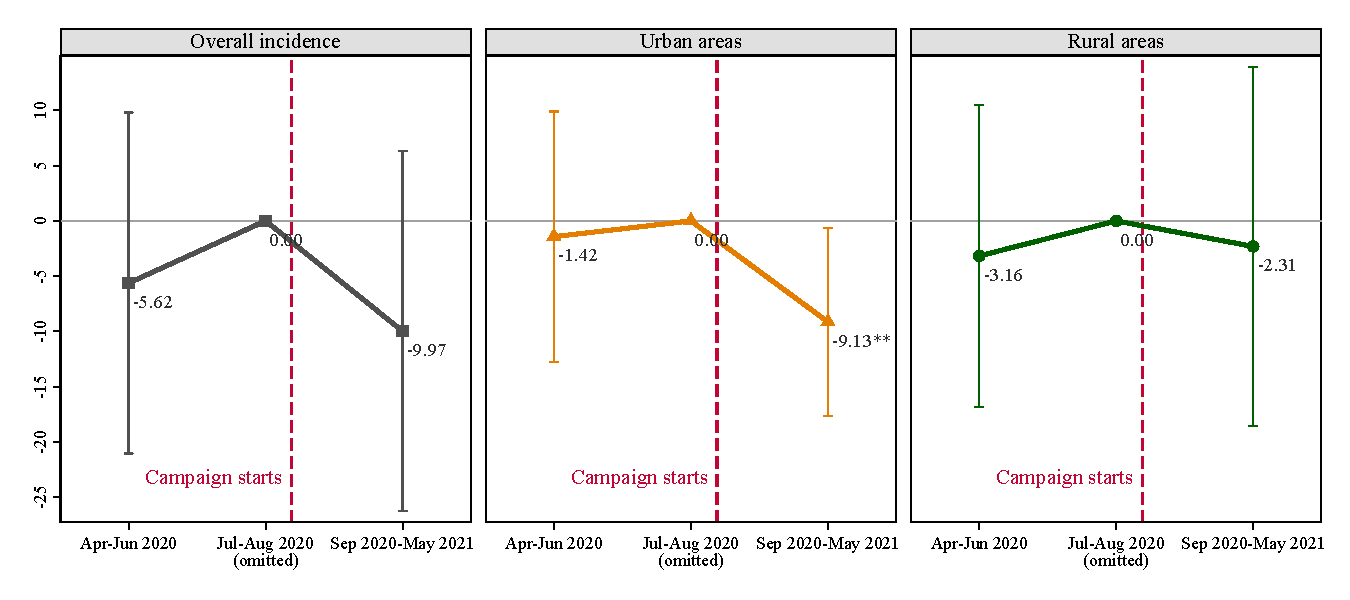
\includegraphics[scale=0.75]{chapters/02-malaria/figures/incidence_dd_trends.pdf}
    \label{fig:incidence}
    \begin{minipage}{16cm}
\scriptsize {Notes: Each point reports the coefficient on the interaction term T$\times$Period, where T is the treatment assignment, and Period is a dummy variable equal to 1 at each period on the graph (i.e., Apr-Jun 2020, Jul-Aug 2020 and Sep 2020-May 2021). The omitted period is Jul-Aug 2020. Each graph reports the results from one regression. Regressions include subdistrict and period fixed-effects, as well as district-level controls interacted with period dummies. Standard errors are clustered at the district level. Bars represent the 95\% confidence intervals.\sym{*} \(p<0.1\), \sym{**} \(p<0.05\), \sym{***} \(p<0.01\)}
\end{minipage}
\end{figure}


The identifying assumption underlying the Difference-in-Differences estimates in Table \ref{tab:incidence} is parallel trends: absent the campaign, malaria incidence would have evolved similarly in treatment and control subdistricts. This assumption is plausible given the cluster-level randomization, and we provide supporting evidence. Figure \ref{fig:incidence} traces treatment-control differences in malaria incidence over time and allows us to assess potential pre-existing divergences before the campaign. Although there appears to be a modest upward pattern in overall incidence in treated relative to control areas before the intervention, these differences are not statistically significant and become smaller when urban and rural areas are examined separately. Overall, the figure is consistent with the parallel trends assumption, showing similar pre-campaign patterns in urban and rural incidence across treatment and control groups. It also shows a decline in urban malaria incidence following the campaign, while the estimated effects in rural areas are much smaller and insignificant. This visual evidence is complemented by the formal pre-trend tests reported in Annex Table \ref{tab:pretrend_checks}. Using only pre-campaign data, both a placebo Difference-in-Differences specification and a linear-trend specification yield coefficients that are small and statistically insignificant for overall, urban, and rural incidence.




\subsection{Placebo Regressions and Robustness Checks}
We begin by examining the sensitivity of the survey-based results to the inclusion of individual- and district-level covariates, and to adjusting for multiple hypothesis testing. Annex Table \ref{tab:all_ols} reports the survey outcomes and shows that the estimated coefficients remain stable when controls are added. To account for the fact that we test multiple survey outcomes, we also report \textit{p}-values adjusted using the Benjamini--Hochberg false discovery rate (FDR) procedure \citep{benjamini1995controlling}. Although precision improves in some cases, the overall pattern of results is unchanged, and the estimates remain statistically insignificant after FDR adjustment. We also assess the sensitivity of the SES-based heterogeneity results to the inclusion of controls and find that the estimates remain highly stable, further supporting the patterns documented in the main text.%\footnote{Results available upon request.}


Because bednet use was measured at baseline, before the campaign began, we also estimate placebo regressions to further validate the randomization. Columns (1)--(2) of Annex Table \ref{tab:placebos} report the results of regressing pre-treatment bednet-use outcomes measured in July and August 2020 on the treatment indicator. The estimates provide additional support for successful randomization: all coefficients are small and statistically insignificant, which also helps alleviate concerns about differential reporting bias.

We also consider whether the survey-based results may be affected by reporting bias. Such bias could arise from repeated survey participation, for example through mere-exposure effects, or from social desirability in self-reported behaviors. Social desirability bias is unlikely to be strongly correlated with campaign exposure, however, because the Facebook and Instagram page used to recruit and survey participants was entirely separate from the MNM campaign page, reducing the likelihood that respondents perceived a connection between the survey and the intervention. As a placebo check, we examine respondents’ perceived risk of contracting COVID-19 in the next year, an outcome unrelated to the campaign, and find no treatment effect (columns (3)--(4) of Annex Table \ref{tab:placebos}). This suggests that campaign exposure did not systematically shift self-reported risk perceptions more broadly.

To assess whether repeated survey exposure may have confounded the results, we examine heterogeneity by ``survey dose'', stratifying respondents into: (i) those who completed only the first wave, (ii) those who completed one to four waves, and (iii) those who completed more than five waves. We then re-estimate the main specification for each group. As shown in Annex Table \ref{tab:bednets_fever_bywaves}, treatment effects remain statistically insignificant across all groups, and the estimates are similar in magnitude and statistically indistinguishable from one another. These findings alleviate concerns that repeated participation is either masking or generating the null results. Finally, the administrative health-facility data are consistent with the survey evidence: measures of malaria incidence and test positivity likewise show no broad overall effects. Given that the survey covered about 8,300 individuals, representing less than 0.01\% of the 116 million residents in the 79 study districts, it is highly unlikely that survey participation itself affected district-level outcomes.

For the health-facility data, we test the robustness of the results to alternative models, samples, and outcome definitions. First, as shown in Table \ref{tab:incidence}, the estimated treatment effects change little with the inclusion of district- and subdistrict-level controls. Second, Annex Table \ref{tab:dd_sensitivity} reports the sensitivity of the estimates to eight alternative population thresholds used to define the subdistrict sample. The effect of the campaign on urban incidence is stable and mostly statistically significant across specifications, with estimated reductions generally around 30\% of the baseline urban incidence rate. By contrast, the coefficient for rural incidence is unstable in sign and generally remains statistically insignificant. Third, Annex Table \ref{tab:incidence_count} considers the absolute number of malaria cases as the dependent variable and includes subdistrict population among the controls. Columns (1)--(3) report estimates from a linear model using the \textit{log} number of cases, while columns (4)--(6) report results from a Poisson model. In both cases, the findings are closely aligned with the main results, indicating that the campaign reduced malaria incidence in urban areas but not in rural ones. For example, the \textit{log} specification implies a roughly 30\% reduction in urban incidence, and the corresponding effect is even larger in the Poisson model; both estimates are statistically significant at the 5\% level.






\section{Mechanisms: Limited Ad Effectiveness or Limited Exposure?} \label{sec:mechanisms}
Taken together, the survey and administrative evidence point to limited average effects of the campaign. At the same time, the post-hoc heterogeneity analysis suggests that the campaign’s measurable impacts were more concentrated among relatively advantaged households and in urban areas, while we find little evidence of impacts among poorer and rural populations, which face higher malaria risk. We interpret these SES and urban-rural patterns as descriptive heterogeneity rather than as evidence that one specific factor explains the difference in effects. We next ask what might explain these differences: did they reflect lower effectiveness of the ad content among poorer and more malaria-vulnerable populations, or lower exposure to the campaign?

%The two explanations have different implications. 
On the one hand, the content may have been less persuasive for higher-risk and more disadvantaged populations, reflecting limitations in the identification of relevant personas or in the tailoring of campaign messages. On the other hand, these populations may have been less likely to receive the ads---for example, because platform delivery algorithms prioritized users with higher expected engagement \citep{lambrecht2019algorithmic,sapiezynski2022algorithms}---which would instead point to limitations in targeting and delivery. To shed light on these mechanisms, we rely on two complementary exercises. First, we study post-campaign ad recall, an imperfect but useful proxy for exposure. Second, we implement a \textit{feed} experiment in which assignment to campaign ads was randomized at the individual level and balanced across socioeconomic predictors, allowing us to assess whether lower- and higher-SES respondents responded similarly when potential exposure was made more comparable.





\subsection{Post-Campaign Recall}

We measured ad recall at the end of the campaign. If exposure differed systematically across groups, we would expect this to be reflected in respondents' ability to remember having seen the ads, although recall also depends on attention and memory. In the endline survey, conducted between December 15, 2020 and January 31, 2021, respondents were asked whether they recalled seeing a Malaria No More (MNM) ad on Facebook or Instagram since August 2020. Table \ref{tab:mnmadrecall_ols} reports the results. Columns (1)--(2) show that treated respondents were 3 p.p. more likely to recall the campaign, corresponding to a 26\% increase relative to the control mean. The logit estimates imply a nearly identical marginal effect. When we split the sample by SES, recall increases significantly by 4.7 p.p. among high-SES respondents (column 3), whereas the corresponding estimate for low-SES respondents is a statistically insignificant 1 p.p. (column 4). While the difference across the two groups is not statistically significant, the estimates are directionally consistent with greater campaign exposure among higher-SES respondents. We view this evidence as suggestive rather than conclusive, since recall is not a direct measure of exposure.


\begin{table}[h!]
    \centering
    \caption{Ad recall at endline} 
%    \vspace{3pt} \begin{minipage}{16cm}
%\footnotesize \it \centering {Y=1 if respondent reported to have seen any ad from Malaria No More on Facebook since last August}
%    \end{minipage}
    \footnotesize
    %\hspace*{-1cm}
    {
\def\sym#1{\ifmmode^{#1}\else\(^{#1}\)\fi}
% Requires in preamble: \usepackage{array}

% Set the width you want for each estimate column here:
\newcommand{\colw}{1.9cm}

\adjustbox{max width=\textwidth}{%
\begin{tabular}{l
    >{\centering\arraybackslash}p{\colw}
    >{\centering\arraybackslash}p{\colw}
    >{\centering\arraybackslash}p{\colw}
    >{\centering\arraybackslash}p{\colw}}
\hline\hline
                &\multicolumn{2}{c}{Full sample}&\multicolumn{1}{c}{High SES}&\multicolumn{1}{c}{Low SES}\\
\cmidrule(lr){2-3}\cmidrule(lr){4-4}\cmidrule(lr){5-5}
                &\multicolumn{1}{c}{(1)}         &\multicolumn{1}{c}{(2)}         &\multicolumn{1}{c}{(3)}         &\multicolumn{1}{c}{(4)}         \\
                &      OLS         &    Logit         &      OLS         &      OLS         \\
\hline
T               &    0.030\sym{**} &    0.266\sym{**} &    0.047\sym{**} &    0.010         \\
                &  (0.014)         &  (0.124)         &  (0.022)         &  (0.021)         \\
\hline

% Center the interaction stats across columns (3)-(4)
\emph{T}$\times$\emph{High SES} coef.
                &                  &                  & \multicolumn{2}{c}{\num{0.039}} \\
\emph{T}$\times$\emph{High SES} p-value
                &                  &                  & \multicolumn{2}{c}{\num{0.253}} \\
\hline

Observations    &     1492         &     1492         &      744         &      748         \\
Adj. R-squared  &    0.000         &                  &    0.004         &   -0.000         \\
Pseudo R-squared&                  &    0.003         &                  &                  \\
Marginal effect &                  &    0.030         &                  &                  \\
Mean in control &    0.114         &    0.114         &    0.111         &    0.117         \\
SD in control   &    0.318         &    0.318         &    0.314         &    0.322         \\
\hline\hline

\multicolumn{5}{p{.75\linewidth}}{\scriptsize Each observation is an individual. The dependent variable equals 1 if the respondent reported to have seen any ad from Malaria No More on Facebook since last August. \(T\) is the treatment indicator. Responses collected in the endline survey between December 15, 2020 and January 31, 2021 are included. State fixed effects are included in all columns. Standard errors are clustered at the district level. \sym{*} \(p<0.1\), \sym{**} \(p<0.05\), \sym{***} \(p<0.01\).}\\
\end{tabular}
}%

}

    \label{tab:mnmadrecall_ols}
\end{table}


Annex Table~\ref{tab:mnmadrecall_ols_heterogeneous} shows that the results are robust to the inclusion of controls (column 1) and to the use of a logit estimator (column 2). The table also explores heterogeneity in ad recall by age and baseline concern about malaria.\footnote{We expect ad recall to be larger among younger respondents, since they spend more time on social media and thus have more exposure to ads. We also expect larger recall rates among respondents with higher levels of concern about getting malaria, since they would pay more attention to malaria-related ads if these appeared on their feeds.} The estimates show that treatment significantly increased ad recall among respondents younger than 26 and among those who reported being at least somewhat worried about malaria at baseline, with effects of 6.9 and 5.6 p.p., respectively. By contrast, the estimated effects are close to zero and statistically insignificant among older respondents and among those who were not concerned about malaria. These findings suggest that the campaign was more salient among younger and more malaria-concerned individuals, or that these groups were more likely to be exposed to the ads.






\subsection{Individual-level \textit{Feed} Experiment}

To distinguish between limited ad effectiveness and limited exposure to the campaign, we embedded a small-scale individual-level study in March--April 2021 at the end of the cross-sectional survey (see Section \ref{sec:data}). The goal of this study was to make potential ad exposure more comparable across respondents with different socioeconomic characteristics. To do so, assignment to the campaign ads was randomized at the individual level and balanced across several predictors of socioeconomic status, including dwelling type, caste, and education, as well as gender and respondents’ district-level treatment assignment in the original MNM campaign. By randomizing assignment within a reachable survey sample and using remarketing to reach most treated respondents, the experiment tests whether the ad content can affect behavior across households with different socioeconomic conditions.


Specifically, at the end of the cross-sectional survey, respondents were asked whether they would be willing to be contacted again within one to three months. To increase statistical power, we also recruited an additional group of participants in March 2021 using the same Meta ads and recruitment procedures as in the earlier survey samples. Among those who agreed to participate, individuals were randomly assigned to treatment or control, with the assignment balanced across the socioeconomic predictors described above. We then used Meta’s remarketing tool to place campaign ads directly in participants’ Facebook and Instagram feeds. In practice, because respondents completed our survey on Messenger, we were able to use anonymous identifiers to create a ``Custom Audience'' for the treatment group.\footnote{Remarketing is a tool offered by major ad platforms through which an ad campaign can be shown to a group of individuals who have previously interacted with the advertiser in some way. This implies that the individual either came directly from an ad to a platform controlled by the advertiser (e.g., a website, app, or chatbot), directly connected their account (e.g., via ``Login with Facebook''), or shared personally identifying data and gave the advertiser permission to use that data for marketing or communication purposes.} We then handed over this audience to MNM, which remarketed ads from its own Meta pages for two weeks, closely mirroring the nationwide campaign.\footnote{This campaign featured the highest-performing ads from the earlier nationwide campaign, which had received a substantial budget (Annex Figure \ref{fig:top_content}). We broadly targeted these ads to all users, regardless of their characteristics.} The remarketing campaign reached 2,119 individuals---about 90\% of the total audience---at least once over the two-week period, with an average frequency of 4.9 ads per person. These ads appeared in users' feeds alongside competing ads and organic content from various sources. Crucially, participants were unaware that the ads had been targeted to them on the basis of their survey participation. As a result, the remarketing campaign closely resembled the nationwide campaign, enhancing the ecological validity of the individual-level study.

Two weeks after the end of the remarketing campaign, we invited respondents to complete a follow-up survey. Our analysis focuses on those who completed this survey; after cleaning, the final sample includes 1,542 respondents (Table \ref{tab:data_cleaning} reports the cleaning procedure). Annex Table \ref{tab:ind_study_balance} presents the distribution of individual and household characteristics across the treatment and control groups. The sample is well balanced on most covariates, including age, gender, education, and bednet ownership. We observe a few imbalances in household size and unemployment, but their normalized differences are small and remain below 0.10.

We focus on two primary behavioral outcomes for which effects could plausibly emerge within our two-week window: bednet use and seeking medical attention in the hypothetical event of a high fever. To facilitate comparison, the survey questions closely mirror those used in the longitudinal panel survey (see Annex \ref{mal-appendix:B}). To limit priming and survey effects, we elicited these outcomes only once, at follow-up.

Our workhorse specification is a linear probability model estimated by Ordinary Least Squares:
\begin{align}
y_{idz} &= \alpha + \beta_{1} \, Individual\,T_{idz} + \beta_{2} \, T_{dz} + \theta_{z} + \epsilon_{idz}.
\end{align}

Here, $i$ denotes an individual residing in district $d$ and state $z$. \textit{Individual T} is the individual-level treatment indicator for the remarketing campaign, while $T$ is the district-level treatment indicator capturing potential persistent effects of the nationwide campaign. $\theta_{z}$ denotes state fixed effects. We report heteroskedasticity-robust standard errors. The coefficient of interest is $\beta_{1}$. We present estimates for the full sample and separately by SES group, using the same classification described above, and report robustness checks with controls and logit estimation.

\subsection{Targeting Matters}

Table \ref{tab:bednets_careseeking_individual} reports the effects of the individual-level remarketing treatment on bednet use and timely treatment seeking. Columns (1)--(3) focus on whether the respondent slept under a mosquito net the previous night, restricting the sample to households owning at least one bednet. In the full sample, the individual-level treatment increases bednet use by 6.9 p.p. $(p<0.05)$. This implies an increase from 65.4\% in the control group to 72.3\% in the treatment group, or about an 11\% increase. The magnitude of this effect is larger than the treatment effect estimated for the nationwide MNM campaign in Section \ref{sec:servey_results}. A plausible explanation is that the cluster-level estimates capture intent-to-treat effects, since only an unknown subset of survey respondents in treated districts was actually exposed to the campaign. By contrast, in the individual-level study the majority of treated respondents (about 90\%) were reached by the remarketing campaign at least once. The estimates in Table \ref{tab:bednets_careseeking_individual} are therefore closer to treatment-on-the-treated effects.

\begin{table}[h!]
    \centering
    \caption{Sleeping under bednet and timely treatment seeking (individual-level study)}
    \footnotesize
    \hspace*{-0.3cm}
    {
\def\sym#1{\ifmmode^{#1}\else\(^{#1}\)\fi}
\adjustbox{max width=\textwidth}{%
\begin{tabular}{l*{6}{c}}
\hline\hline
                &\multicolumn{3}{c}{Respondent used bednet the night before}&\multicolumn{3}{c}{Timely treatment seeking if high fever}\\\cmidrule(lr){2-4}\cmidrule(lr){5-7}
                &\multicolumn{1}{c}{(1)}         &\multicolumn{1}{c}{(2)}         &\multicolumn{1}{c}{(3)}         &\multicolumn{1}{c}{(4)}         &\multicolumn{1}{c}{(5)}         &\multicolumn{1}{c}{(6)}         \\
                &Full sample         & High SAS         &  Low SAS         &Full sample         & High SAS         &  Low SAS         \\
\hline
Individual T    &    0.069\sym{**} &    0.074\sym{*}  &    0.077\sym{**} &    0.025\sym{**} &    0.029         &    0.023         \\
                &  (0.029)         &  (0.043)         &  (0.038)         &  (0.013)         &  (0.020)         &  (0.016)         \\
T               &    0.014         &    0.051         &   -0.007         &    0.005         &    0.012         &    0.006         \\
                &  (0.029)         &  (0.043)         &  (0.039)         &  (0.013)         &  (0.020)         &  (0.016)         \\
\hline
\emph{Ind. T}$\times$\emph{High SES} coef.&                  &\multicolumn{2}{c}{\num{-0.006} }                          &                  &\multicolumn{2}{c}{\num{0.005}  }                         \\
\emph{Ind. T}$\times$\emph{High SES} p-value&                  &    \multicolumn{2}{c}{0.911}                           &                  &    \multicolumn{2}{c}{0.845}                           \\\hline
Observations    &     1043         &      520         &      523         &     1542         &      770         &      772         \\
Adj. R-squared  &    0.003         &   -0.001         &    0.005         &    0.005         &    0.022         &   -0.002         \\
Mean in control &    0.654         &    0.599         &    0.704         &    0.921         &    0.907         &    0.934         \\
SD in control   &    0.476         &    0.491         &    0.457         &    0.270         &    0.291         &    0.248         \\
\hline\hline
\multicolumn{7}{p{0.95\linewidth}}{\scriptsize Each observation is an individual. \(Individual\,\,T\) is the individual-level treatment indicator for the remarketing campaign. \(T\) is the indicator of district-level treatment assignment. The outcome in columns (1)--(3) is an indicator equal to one if the respondent reports having slept under a bednet the night before the survey; the sample is restricted to households owning at least one bednet. The outcome in columns (4)--(6) is an indicator equal to one if the respondent reports that they would seek treatment within 24 hours if they or a family member experienced a high fever. The SES index is constructed using Principal Component Analysis (PCA) based on housing quality, access to health facilities, education, caste status, air conditioning ownership, and standardized household size. The index is standardized and split at the median to define High and Low SES groups. Columns (1) and (4) report full-sample estimates. Columns (2)--(3) and (5)--(6) report subgroup-specific treatment effects by SES. The table also reports the interaction coefficient \(Individual\,\,T \times High\,\,SES\) from a specification that includes the standalone indicators \(Individual\,\,T\) and \(High\,\,SES\).  Heteroskedasticity-robust standard errors are reported in parentheses. \sym{*} \(p<0.1\), \sym{**} \(p<0.05\), \sym{***} \(p<0.01\)}\\
\end{tabular}
}%

}

    \label{tab:bednets_careseeking_individual}
\end{table}



Columns (2)--(3) show that these effects are very similar across socioeconomic groups. The estimated treatment effect on bednet use is 7.4 p.p. among high-SES respondents and 7.7 p.p. among low-SES respondents. Consistent with this, the interaction between the individual treatment and the high-SES indicator is close to zero and statistically insignificant ($p = 0.911$). Thus, when assignment to the remarketing campaign is randomized and potential exposure is made more comparable across groups, we find no evidence that the campaign is less effective among lower-SES households. This pattern supports the interpretation that weaker nationwide effects among more disadvantaged respondents were driven primarily by differential exposure rather than lower ad effectiveness.

Columns (4)--(6) turn to treatment-seeking intentions in the event of a high fever (100.4$^\circ$F / 38$^\circ$C or above). The dependent variable equals one if the respondent reports that they would seek treatment within 24 hours. In the full sample, the individual-level treatment increases timely treatment seeking by 2.5 p.p. $(p<0.05)$, corresponding to a 2.7\% increase relative to the control mean. The point estimates are similar across SES groups: 2.9 p.p. for high-SES respondents and 2.3 p.p. for low-SES respondents. However, these subgroup estimates are imprecisely estimated, likely reflecting the loss of power from splitting the sample. The interaction between the individual treatment and the high-SES indicator is again small and statistically insignificant ($p = 0.845$), providing no evidence of heterogeneous treatment effects by SES.

Moreover, across both outcomes, we include the district-level treatment indicator from the nationwide MNM campaign. These coefficients are small and statistically insignificant throughout, suggesting limited persistent effects of the earlier campaign within this sample. Annex Table \ref{tab:bednets_careseeking_individual_extra} shows that the results are robust to the inclusion of controls and to the use of the Logit estimator (Columns 1--2 and 5--6). In addition, Columns 3--4 and 7--8 estimate the effects separately for individuals residing in control and treatment districts of the nationwide campaign and show that the estimated effects are concentrated among respondents in control districts. %, consistent with the idea that those in treatment districts may already have been partially exposed to similar messages during the earlier campaign.

Overall, the individual-level experiment yields two main insights. First, among users assigned to and largely reached by the remarketing campaign, the ads increase both protective behavior and timely treatment-seeking intentions. Second, once potential exposure is made more comparable across respondents with different socioeconomic backgrounds, the treatment effects are similar across higher- and lower-SES households. Taken together, these findings provide evidence that insufficient and differential exposure contributed to the limited average effects observed in the nationwide campaign.


\section{Discussion and Implications for Practitioners}
Our results suggest that the nationwide malaria prevention campaign generated limited average effects, with detectable impacts concentrated among relatively less vulnerable and more connected populations. A plausible interpretation of this pattern is the presence of targeting and delivery frictions: in the absence of explicit targeting toward high-risk users, the platform’s delivery algorithm may have allocated impressions disproportionately toward users who were cheaper and easier to reach, rather than toward those most exposed to malaria risk. This concern is particularly relevant because the nationwide campaign was optimized for engagement. For a public-health intervention, that objective is imperfect, since it may direct spending toward users who are more likely to click or react online rather than toward those for whom the expected health gains are greatest. Our individual-level experiment reinforces this interpretation. When assignment to the remarketing campaign is randomized and potential exposure is made more comparable across respondents with different socioeconomic characteristics, we detect positive effects in the overall sample and no clear evidence of heterogeneous effects by SES. This pattern is more consistent with targeting and delivery frictions than with large differences in the effectiveness of the ad content itself.

Additional evidence is consistent with this mechanism. Our district-level analysis of recruitment ad costs (Table \ref{tab:correlates_recruitment}) shows that the cost per thousand impressions (CPM) was systematically lower in larger and more populous districts, and in districts that were more socioeconomically advantaged, with a higher share of households living in solid dwellings and greater mobile-phone penetration. Because the recruitment ads were also optimized for engagement-related objectives, much like the nationwide malaria campaign, these cost patterns are informative about likely delivery dynamics. Taken together, they suggest that engagement- and cost-based delivery tilted exposure toward relatively advantaged and more connected populations, helping explain why the campaign produced detectable effects primarily among higher-SES households and in urban areas. At the same time, we cannot identify the precise source of the differential exposure observed in the nationwide campaign. Higher CPM may reflect lower social media use among more vulnerable users, smaller reachable audiences, poorer internet connectivity, or differences between vulnerable users on the platform and vulnerable users in the broader population.

The main managerial implication is therefore not that social media campaigns cannot work for vulnerable populations, but that achieving such impacts may require more deliberate targeting and a willingness to incur higher delivery costs than an engagement-maximizing strategy would imply. More broadly, our findings point to a three-step approach for practitioners. First, organizations should invest in formative research to identify the populations for whom the intervention is likely to generate the greatest gains, as well as the groups that are systematically harder and costlier to reach. Second, they may need to go beyond the basic targeting tools offered by ad platforms and rely on more advanced options---such as lookalike models or first-party-data-based custom audiences---to improve inclusion of underserved groups in campaign delivery. Third, campaign managers should explicitly weigh the trade-off between maximizing on-platform engagement and achieving meaningful off-platform behavioral change. In settings like ours, higher delivery costs may be precisely the price of reaching those who stand to benefit the most.

Addressing information gaps and building technical capacity is important, but may not be sufficient. Managerial incentives also need to be realigned. When marketing teams are evaluated primarily on engagement metrics, there is little incentive to invest in reaching harder-to-engage and higher-cost populations, even if these groups stand to benefit the most. Moreover, ongoing changes in privacy policies that restrict access to the data needed for targeting and measurement may further complicate the use of sophisticated campaign-design and evaluation tools. To better align social media campaigns with public-health goals, incentive structures should incorporate offline outcomes as key performance indicators. While reaching high-risk populations may entail higher delivery costs, the developmental return per person reached is likely to be substantially greater.

\section{Cost-effectiveness}

In this section, we provide a benchmark calculation of the campaign’s cost-effectiveness based on the administrative health-facility results, which capture objectively recorded malaria outcomes at the population level. We report two scenarios. The first uses the estimated reduction in overall malaria incidence from Table \ref{tab:incidence}; the second uses the reduction in urban incidence, which is the more precisely estimated effect and corresponds to the setting in which the campaign’s health effects are most clearly detected. Using the most conservative estimates from Table \ref{tab:incidence}, the campaign reduced malaria incidence by 3.12 cases per million people per month in the overall sample and by 6.10 cases per million people per month in urban areas. Interpreting these estimates as average monthly effects over the post-treatment period from September 2020 to May 2021, this implies cumulative reductions of 28.08 and 54.90 officially recorded malaria cases per million people, respectively.

To obtain an approximate campaign-wide benchmark, we extrapolate these effects from the three study states to the 22 states targeted by the MNM national campaign. This extrapolation assumes that the effectiveness observed in the study states is informative about the broader rollout and should therefore be interpreted cautiously. With a total population of roughly 1.2 billion across the 22 campaign states, and excluding approximately 100 million residents in control districts within the study states, the campaign’s potential reach was about 1.1 billion individuals. Under these assumptions, the implied number of officially recorded malaria cases averted ranges from 30,888 under the overall-incidence estimate to 60,390 under the urban-incidence estimate.

The total advertising cost of the national campaign was US\$202{,}000. Dividing this figure by the implied number of averted cases yields a cost per officially reported malaria case averted of about US\$6.50 under the overall-incidence estimate and about US\$3.40 under the urban-incidence estimate. We view these figures as useful benchmarks rather than exact welfare estimates. On the one hand, they are likely to overstate the cost per true case averted because malaria is substantially under-reported in India: the World Malaria Report suggests that true incidence is roughly 22 times higher than officially recorded incidence \citep{world2021malaria}. Accounting for under-reporting would reduce the implied cost per estimated case averted to well below one dollar. On the other hand, the broader extrapolation assumes that the effects observed in the study states generalize to the full national campaign.

While the focus here is on direct advertising costs,\footnote{This follows common practice in the marketing literature. The estimated cost of training sessions, implementation, and project management provided by the social media marketing firm—including nine months of technical support—was US\$44{,}200. This excludes the cost of ad design.} it is useful to compare these figures with those reported for related health communication efforts. For example, the implied cost per officially reported malaria case averted is of a similar order of magnitude to the costs reported for social media campaigns promoting COVID-19 vaccination in developed-country settings \citep{atheycovid2023}. It is also comparable to published estimates for more traditional malaria-prevention interventions such as the distribution of insecticide-treated nets \citep{conteh2021costs}, while differing from those interventions in that the mechanism here operates through information and behavior change rather than through direct provision of prevention tools.

The broader implication is that social media campaigns can be cost-effective public-health tools, but their cost-effectiveness depends critically on who is reached. In our setting, the most favorable cost-effectiveness estimates come from urban areas, where the campaign generated detectable reductions in malaria incidence. In lower-connectivity and harder-to-reach populations, the campaign produced little detectable health impact, implying that digital advertising should be viewed as a complement to, rather than a substitute for, offline malaria-control efforts. At the same time, our mechanism results suggest that better targeting and delivery could improve the equity of such campaigns by extending exposure to populations with higher expected health gains. Whether this would also improve cost-effectiveness is ultimately an empirical question, since the added health benefits from reaching more vulnerable groups must be weighed against the likely higher ad costs.

\section{Conclusions}
Social media campaigns are increasingly used to pursue public-health objectives, yet measuring their effectiveness remains difficult. Platform metrics such as clicks, reactions, and ad recall provide only a partial picture when the outcomes of interest are offline behaviors and health. Malaria prevention campaigns illustrate this challenge particularly clearly. Malaria disproportionately affects poorer and more rural populations in India, but these are also the populations that may be harder or more costly to reach through engagement-optimized digital advertising. Assessing effectiveness therefore requires going beyond platform data and measuring whether campaigns change real-world prevention and treatment behaviors.

In this paper, we evaluate a nationwide malaria prevention campaign implemented by Malaria No More on Facebook and Instagram in India. The campaign promoted bednet use and timely treatment-seeking through behaviorally informed ads tailored to different audience personas. It reached roughly 130 million users over six months, with an average frequency of 3.6 impressions per reached user. To study its effects, we combine a district-level cluster-randomized design with original survey data, administrative health-facility records, and a follow-up individual-level feed experiment.

Our main finding is that the campaign generated limited average effects. In the survey data, average effects on malaria-related protective behaviors, treatment-seeking, and self-reported incidence are generally small and statistically insignificant. At the same time, post-hoc heterogeneity analyses suggest that detectable effects were more concentrated among relatively advantaged households. In particular, bednet use increased during the campaign and self-reported malaria incidence declined afterward among higher-SES households, whereas estimates for lower-SES households are small and indistinguishable from zero. Administrative data point to a related urban-rural pattern: we find no clear overall decline in malaria incidence, but monthly incidence in urban health facilities fell by 6.2 cases per million people, about one-third of the pre-treatment urban baseline, with no detectable effect in rural areas.

These patterns raise an important question: were the ads ineffective for the populations most at risk, or were those populations less likely to be exposed? To shed light on this issue, we conducted a second experiment that randomized assignment to ads at the individual level using the platform's remarketing tools. In that setting, where potential exposure was made more comparable across SES groups, the campaign increased bednet use and timely treatment-seeking intentions, with no detectable differences by socioeconomic status. Taken together, the evidence is consistent with targeting and delivery frictions contributing to the limited average effects of the nationwide campaign.

One limitation of the study is that the intervention took place during the first year of the COVID-19 pandemic. This context may affect external validity, since health-care access, media use, and risk perceptions were unusually shaped by the pandemic. Still, it is unlikely to threaten the internal validity of the experimental design.

Overall, our findings provide a cautious assessment of what social media advertising can achieve in public health. The results suggest that such campaigns can affect behavior and may be cost-effective in some settings, but that engagement-based delivery does not necessarily direct exposure toward the populations with the highest expected health gains. More broadly, the paper shows the value of combining first-party survey data, administrative outcomes, and experimental variation in delivery to evaluate digital campaigns beyond platform metrics. This approach can help organizations measure real-world impact and design more deliberate targeting strategies when privacy constraints and platform optimization limit the reach of standard advertising tools.

\section*{\normalsize Funding and Competing Interests}
\normalsize This research has received funds from the World Bank’s Development Impact Department (DIME) and Facebook’s Campaigns for a Healthier World initiative. Three authors do not have any competing interests to this work. One author has ownership interests in Virtual Lab LLC, a company that uses the open-source methodology described in the paper. 



%\printbibliography
%\addbibresource{./bibs/experimental-design.bib}
%\bibliography{./bibs/digital-ads.bib}
%\bibliography{./bibs/extra.bib}


\clearpage
%\section*{Appendix}

\section{Content Development and Campaign Management}
\label{mal-appendix:A}
\setcounter{figure}{0}
\renewcommand{\thefigure}{A\arabic{figure}}
\renewcommand{\theHfigure}{A\arabic{figure}} % for 'hyperref'

\subsection{Developing content for different personas}
Data insights from public posts revealed that women tended to emphasize family and protection against mosquitoes. Hence, the content development team worked to develop content that women would find engaging; this included content highlighting children and motherhood. Some ads outlined the detrimental effects that malaria can have on pregnant women.

\begin{figure}[h]
	\centering
    \caption{Examples of content to activate women}
	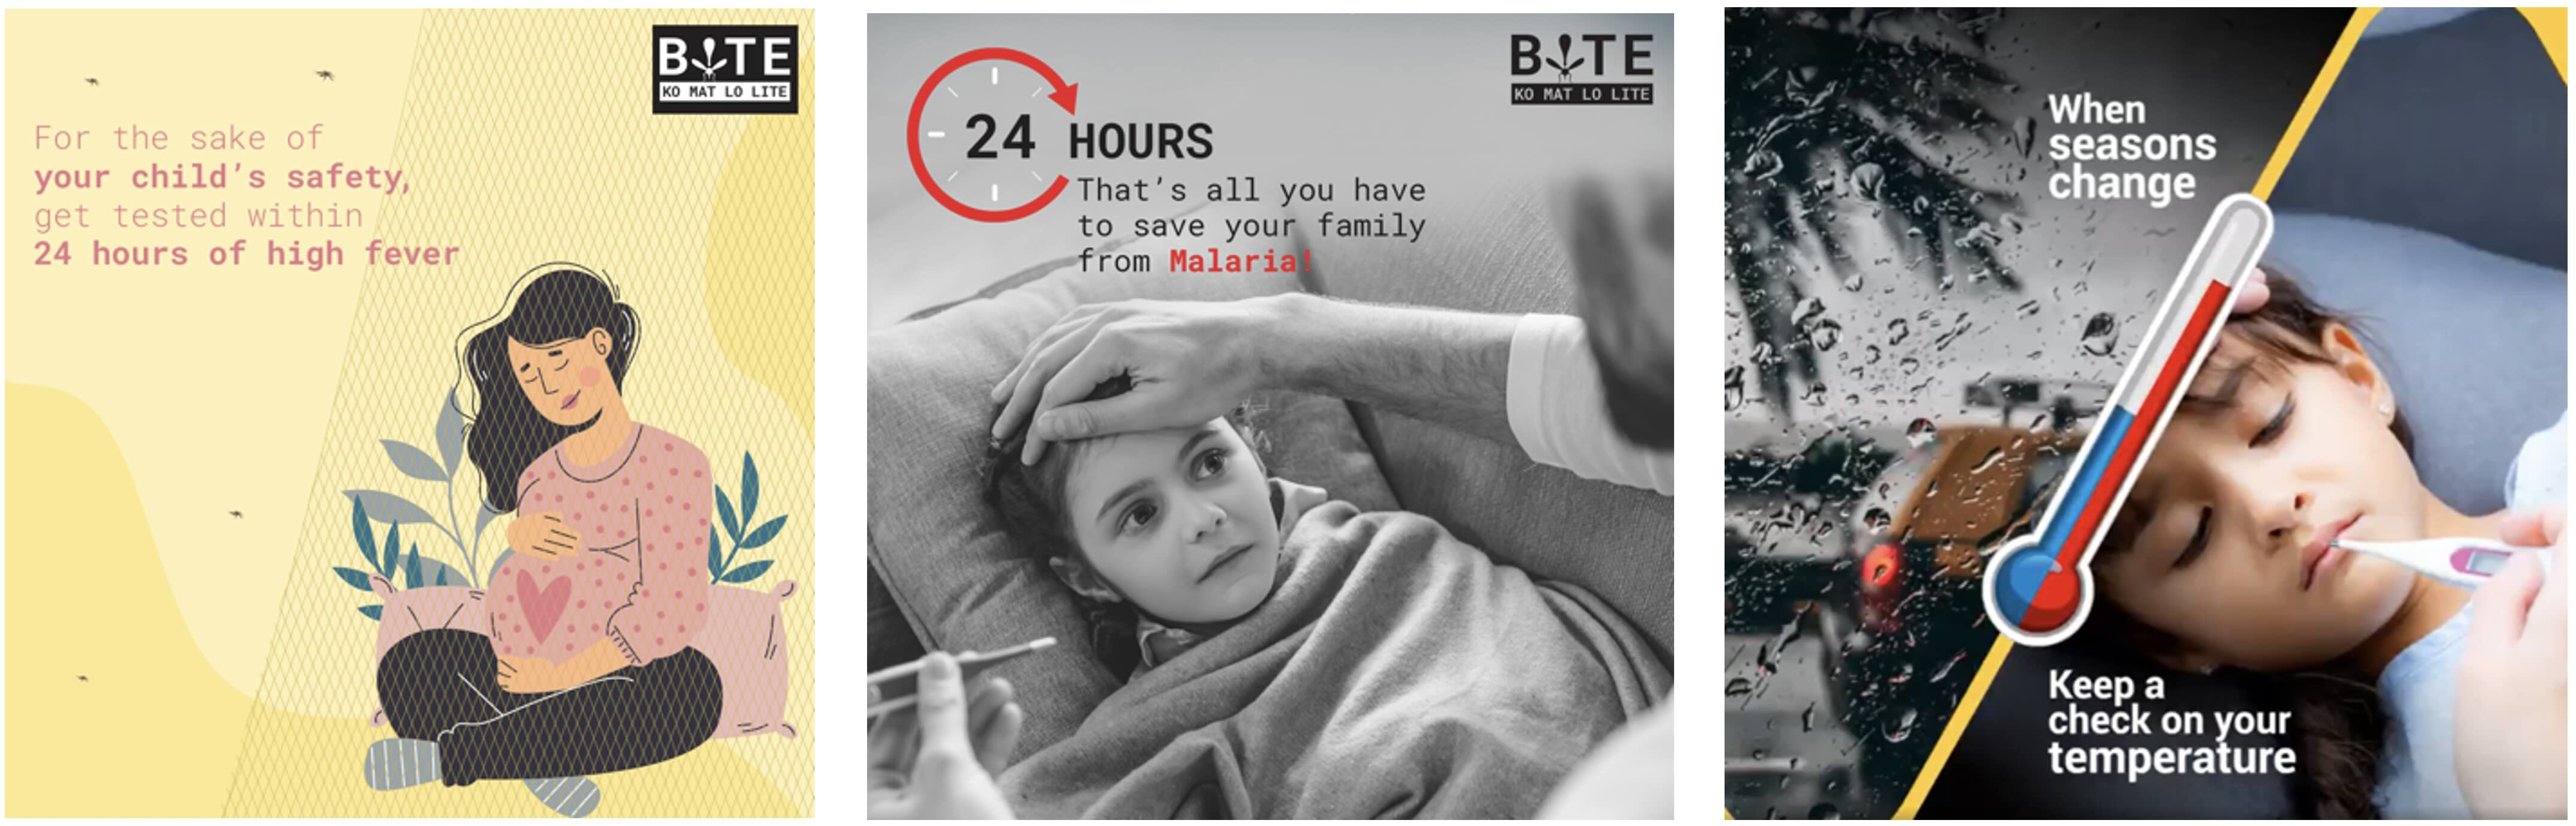
\includegraphics[width=16cm]{chapters/02-malaria/figures/Women}
     \label{fig:women}
\end{figure}

Men, on the other hand, tended to engage more on non-personal aspects of campaigns, such as government, healthcare, symptoms, treatment, and awareness days. Content was also developed to engage male audiences including content which featured a popular sport cricket.

\begin{figure}[h]
	\centering
    \caption{Examples of content to activate men}
	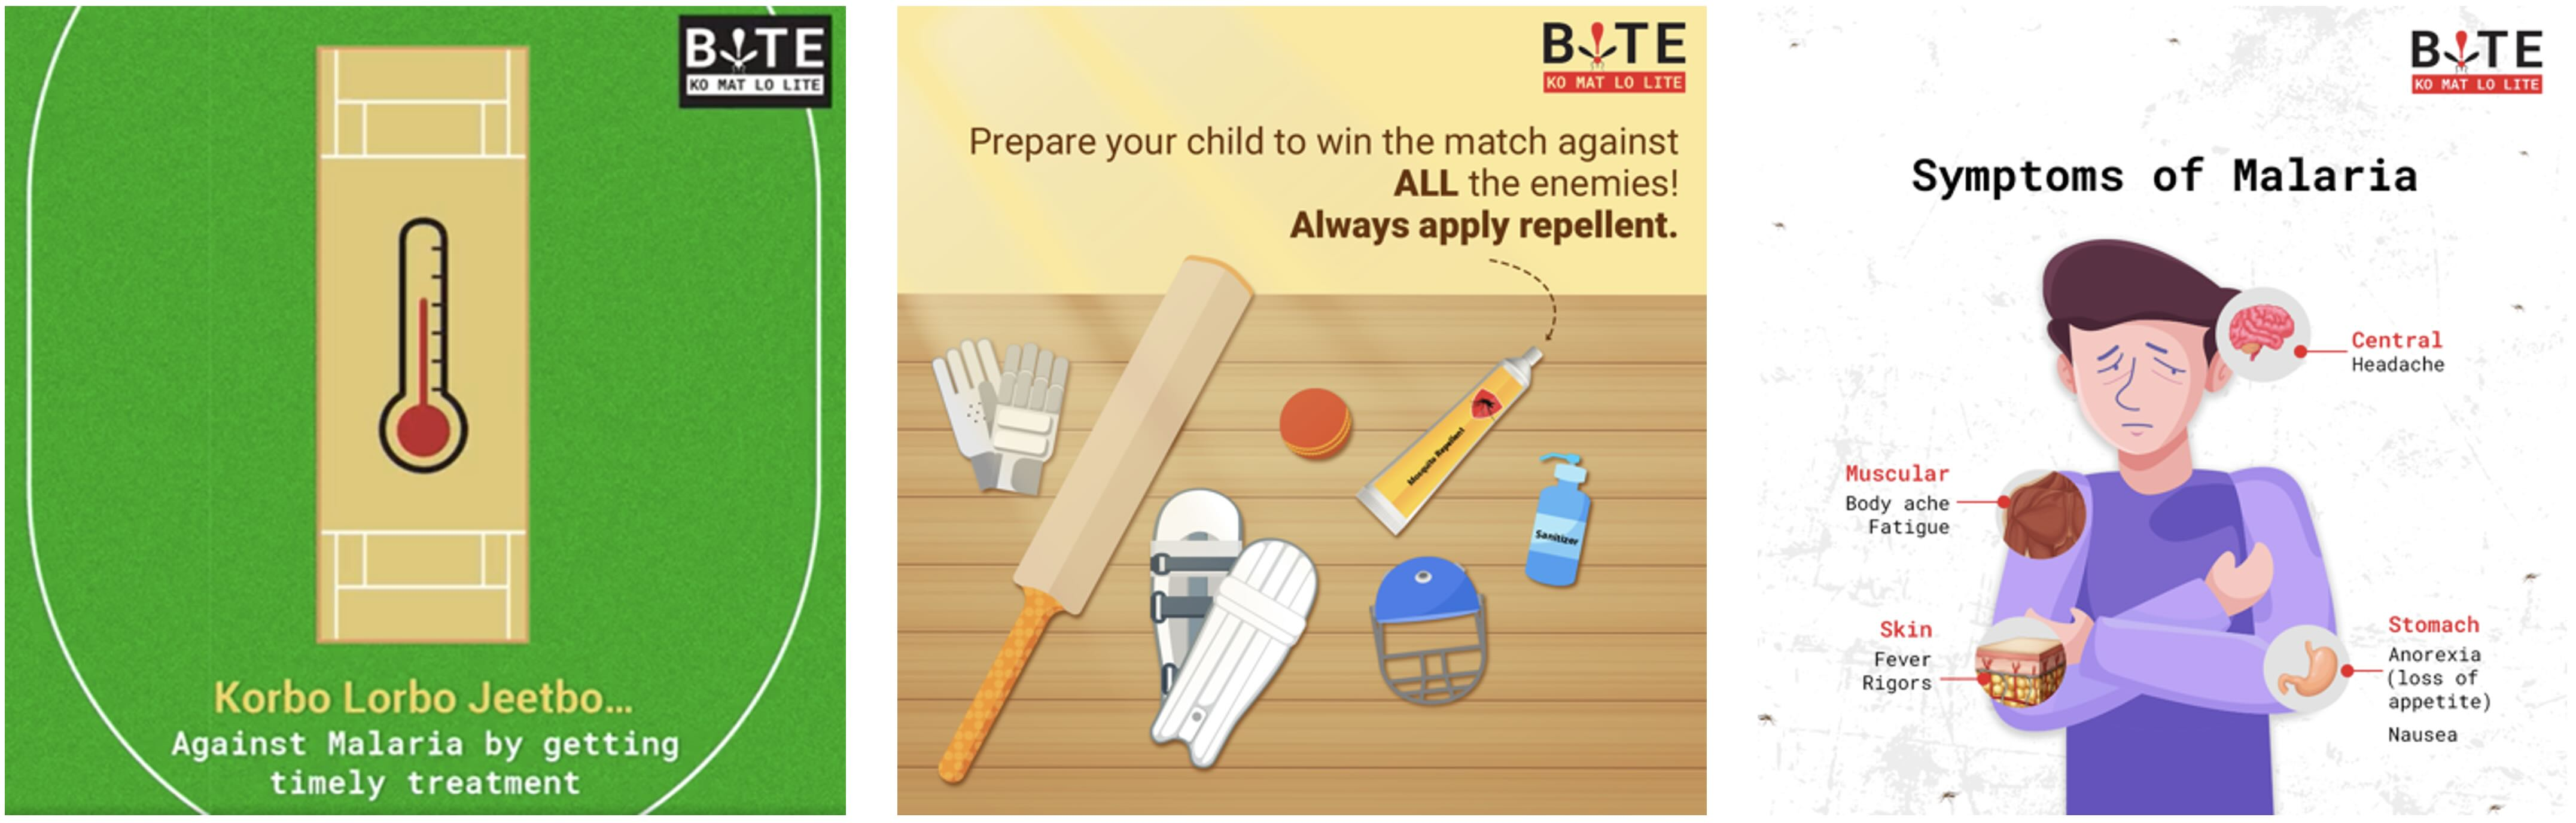
\includegraphics[width=16cm]{chapters/02-malaria/figures/Men}
\end{figure}


Younger audiences, especially in the 18-24 age bucket, were posting about malaria and other mosquito-borne diseases at a lower rate when compared to older people. The MNM team made a conscious effort to use meme-styled content and humor to engage this audience. 

\begin{figure}[h]
	\centering
    \caption{Examples of content to activate younger audiences}
	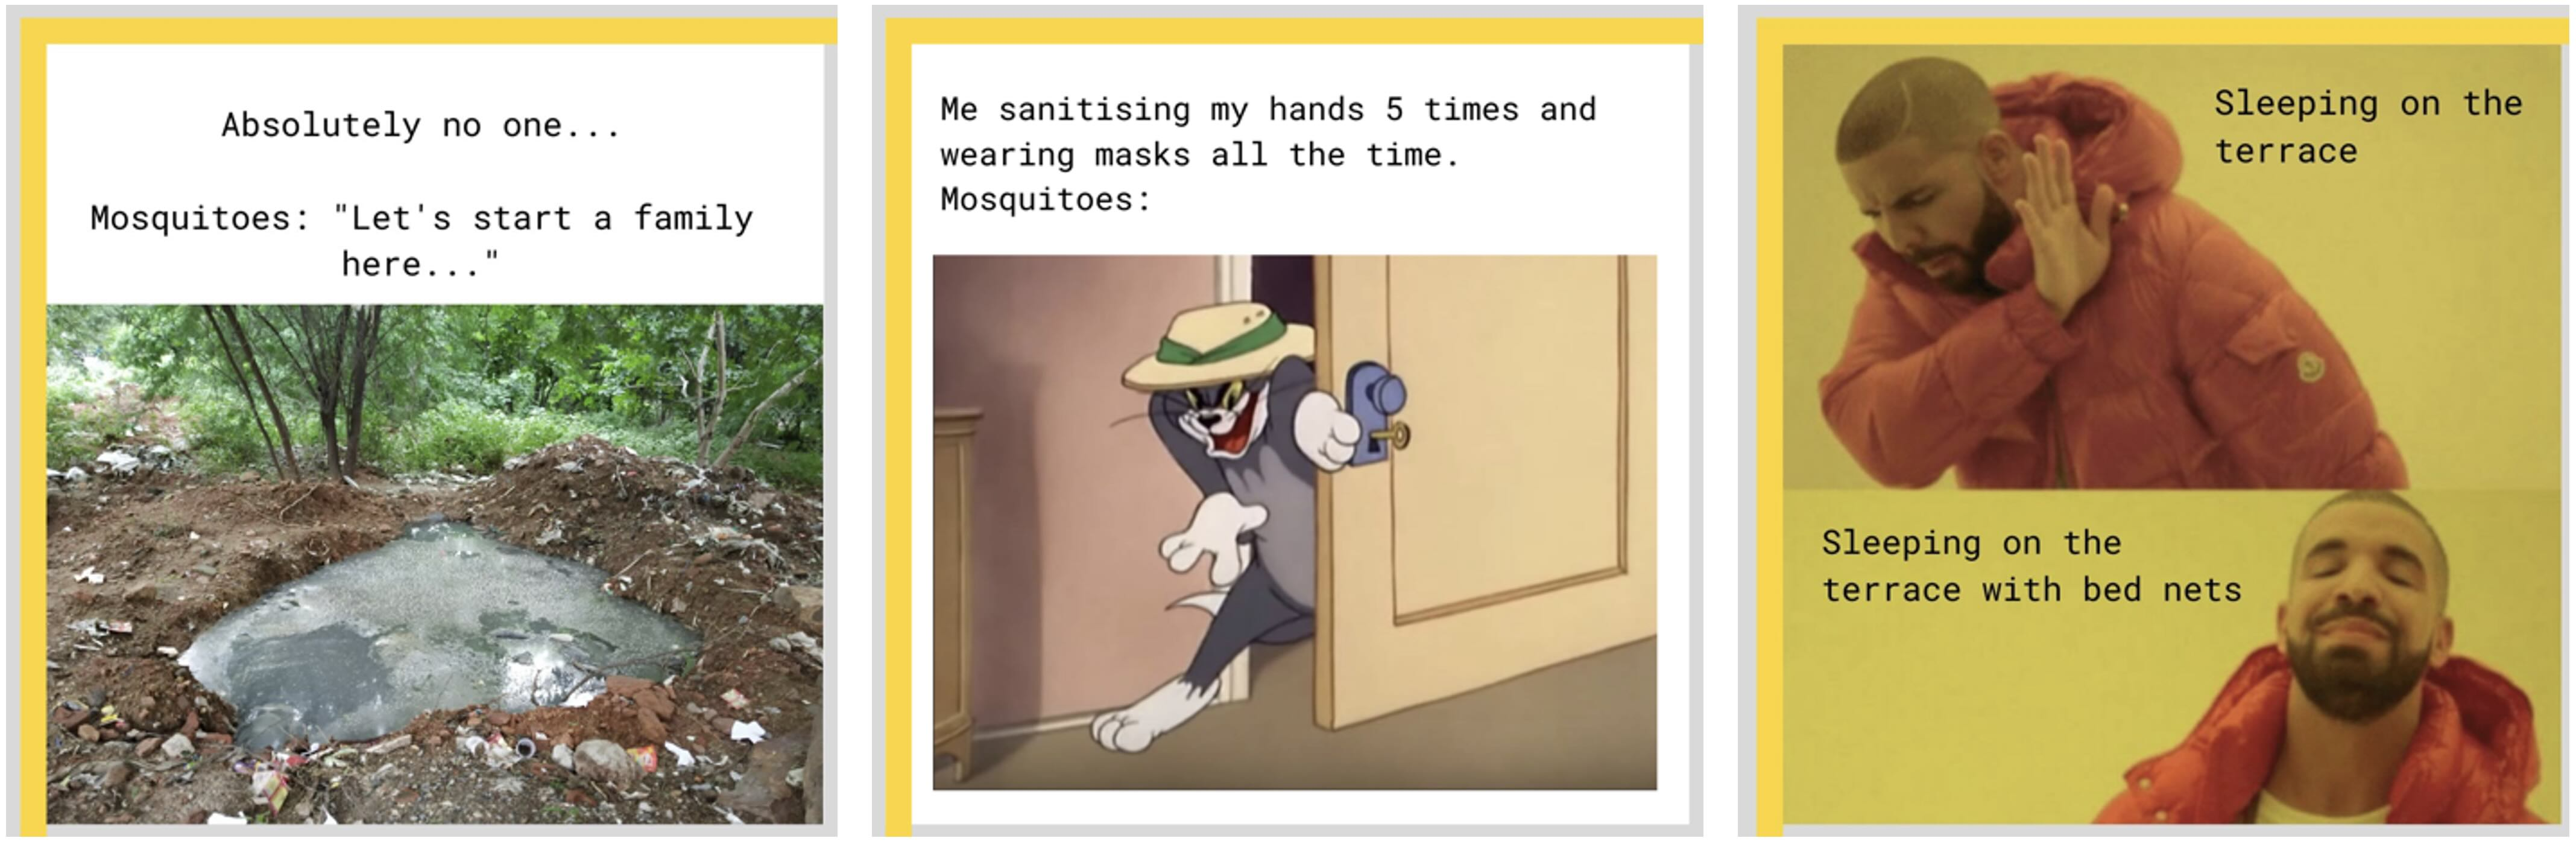
\includegraphics[width=16cm]{chapters/02-malaria/figures/Young}
\end{figure}


The data insights demonstrated that older people were disproportionately more likely to post about malaria and other mosquito-borne disease; this made older people important advocates for promoting the campaign’s objectives. Thus, content was developed specifically for grandparents encouraging them to have their grandchildren tested if they experience malaria symptoms.

\begin{figure}[h]
	\centering
    \caption{Examples of content to activate older audiences}
	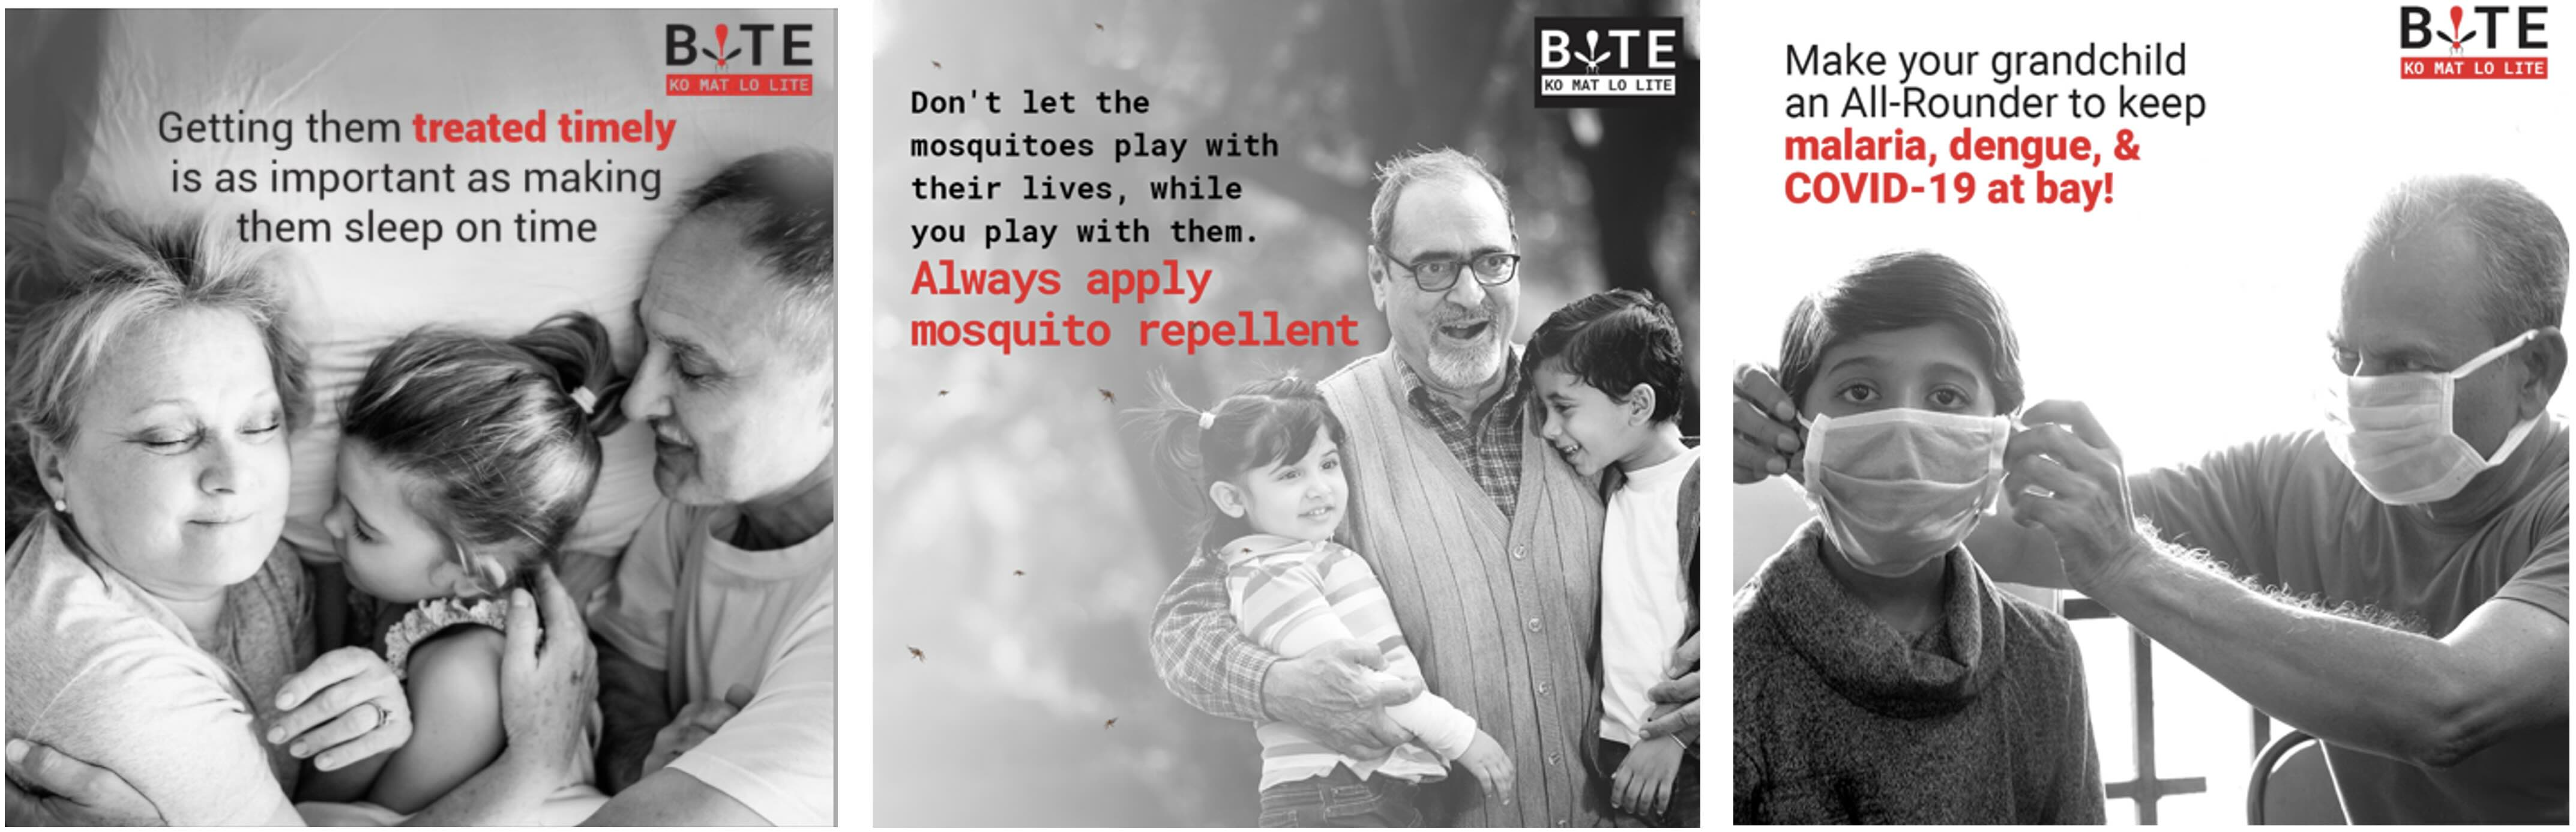
\includegraphics[width=16cm]{chapters/02-malaria/figures/Old}
\end{figure}

The insights revealed that in rural areas, people were posting about malaria and other mosquito-borne diseases at a lower rate than people in urban areas; this finding underscored the need to produce resonant content for rural audiences since malaria disproportionately occurs in rural areas. Furthermore, less urbanized areas were found to post less about mosquito-borne disease in English; this demonstrated the need to have content in other languages including Hindi and Hin-glish. Moreover, analysis of public posts revealed that rural residents highlighted an appreciation for ASHAs (community health workers).

\begin{figure}[h!]
	\centering
    \caption{Examples of content for rural audiences}
	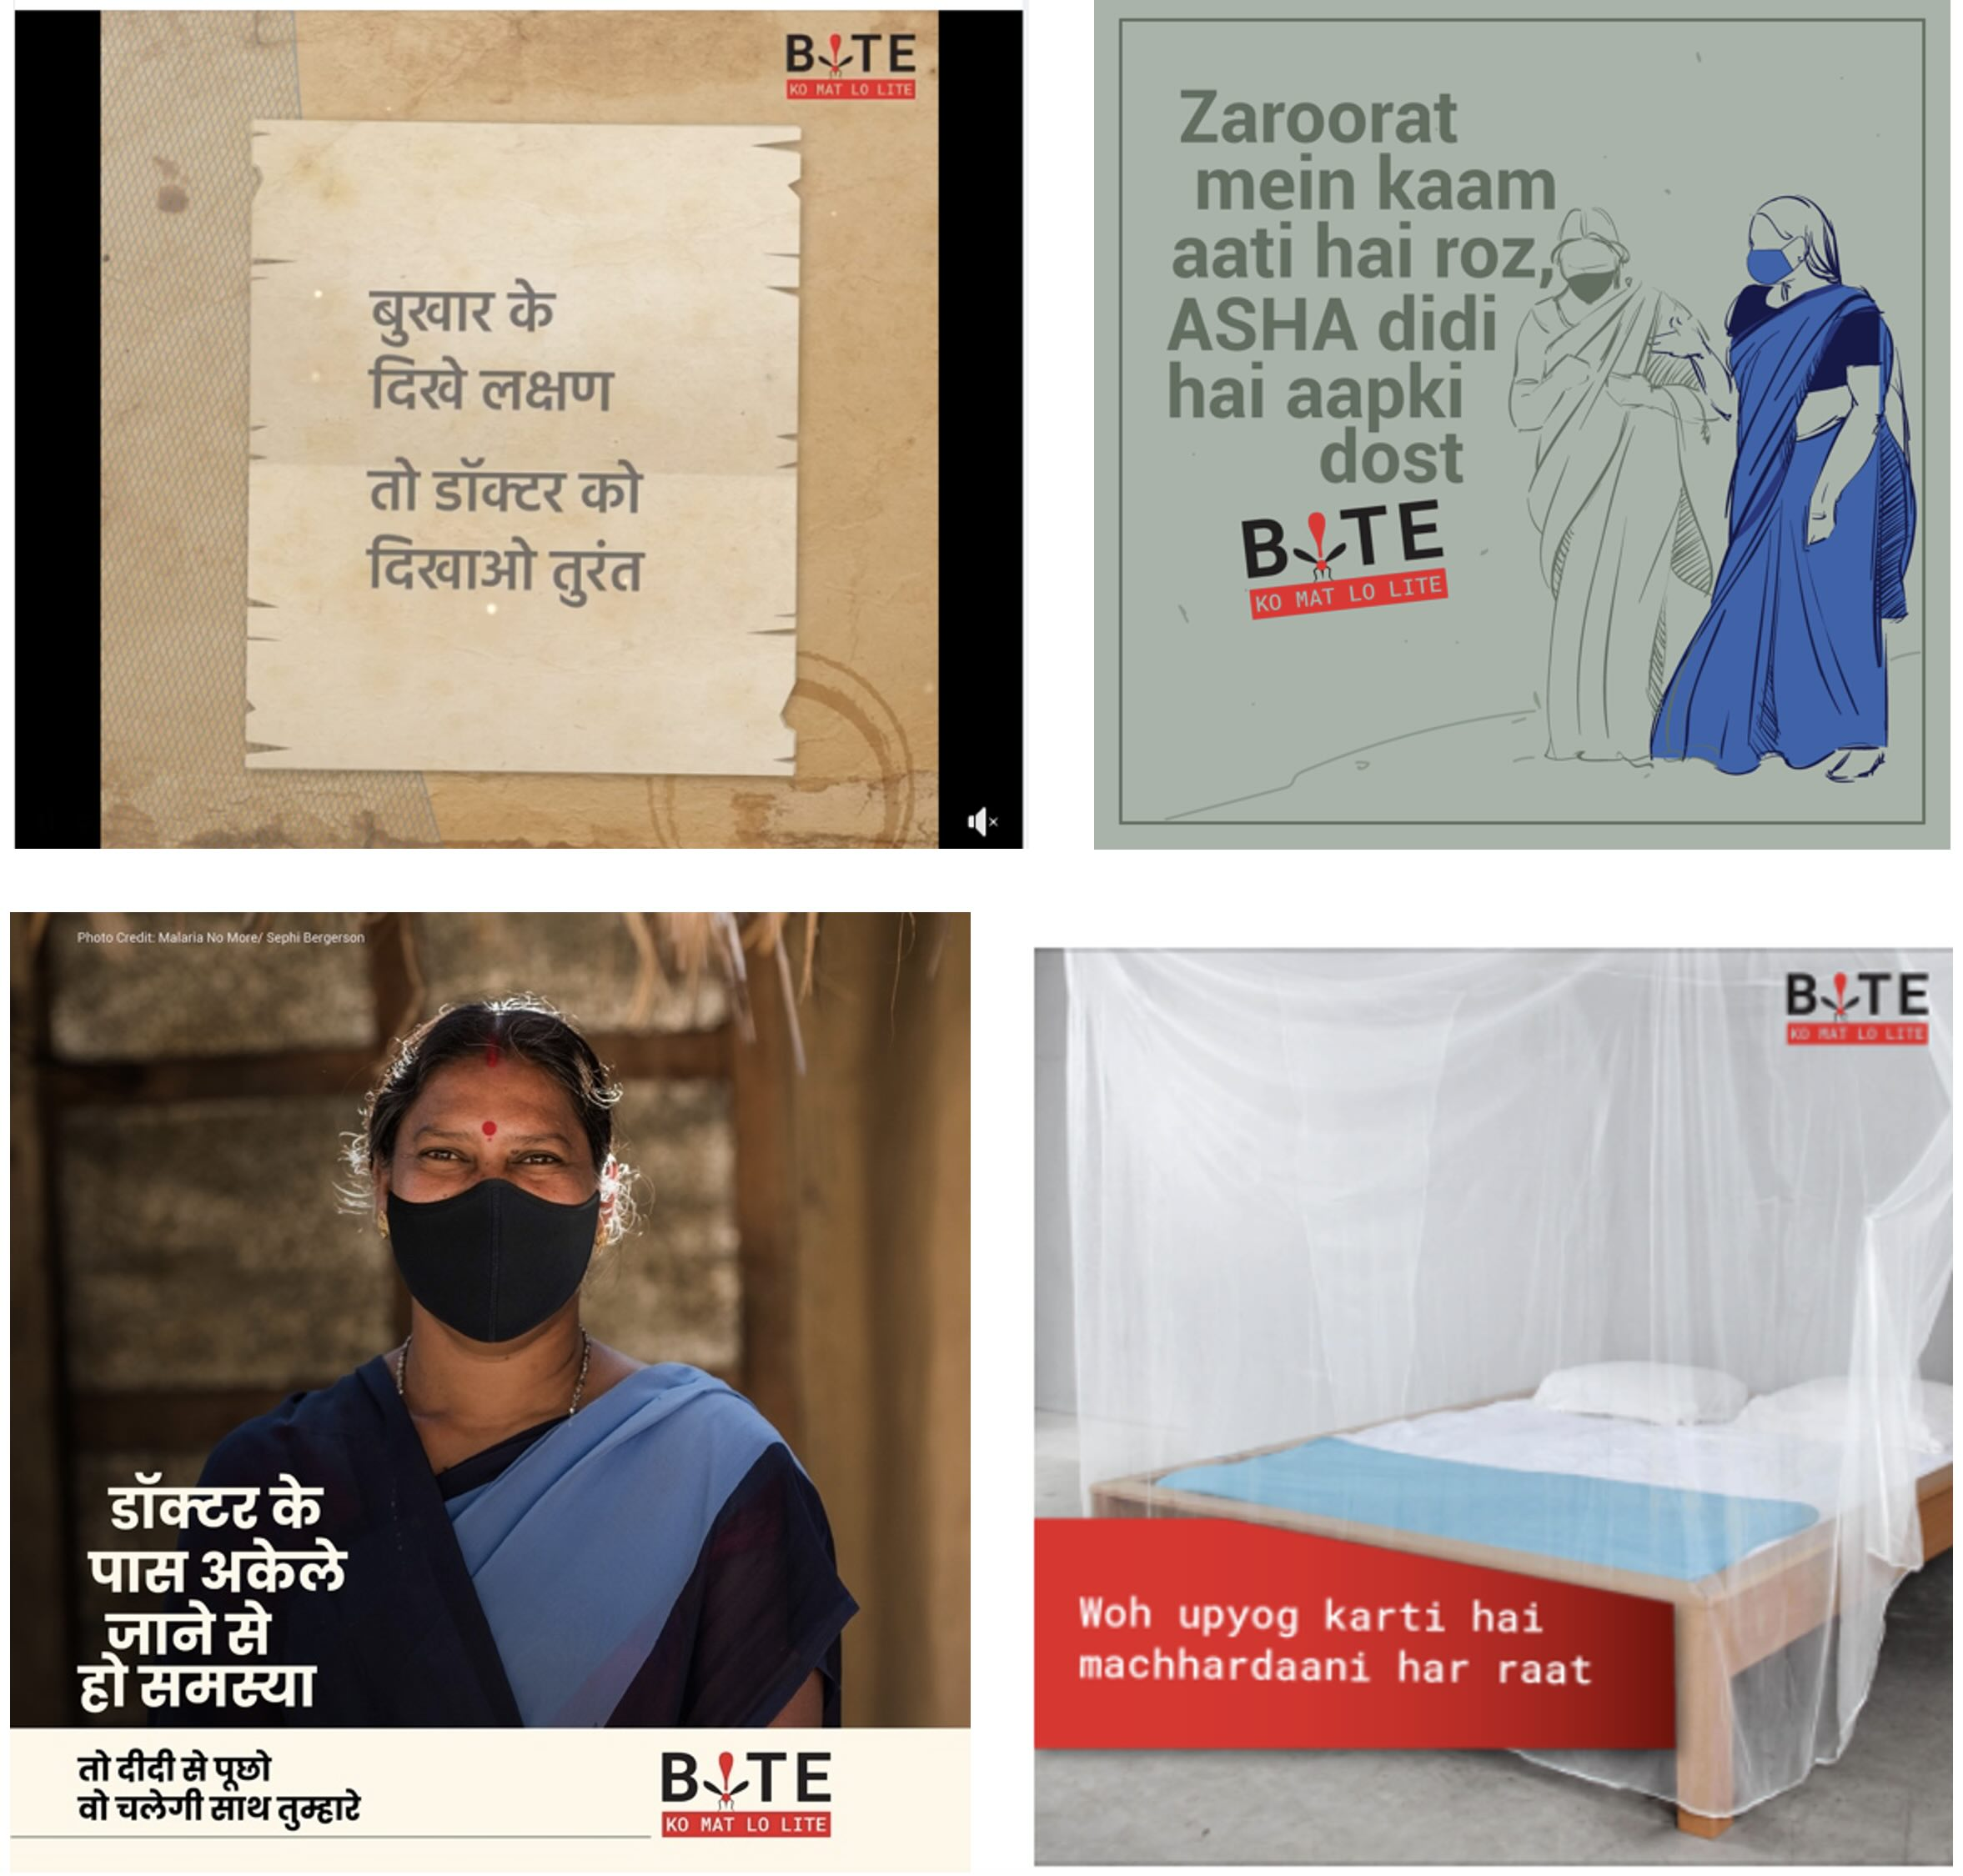
\includegraphics[width=16cm]{chapters/02-malaria/figures/Rural}
\end{figure}


The campaign occurred during the context of the COVID-19 pandemic and one of the main goals was to limit the rise of malaria fatalities during COVID-19 by encouraging people to engage in preventative behavior and to seek testing. Moreover, several symptoms of COVID-19, such as fever, are similar to symptoms for malaria; this further underscored the need for people to get tested. Analysis of posts showed that a large number of mosquito-borne disease posts also mentioned COVID-19, with many posts mentioning the continued threat of malaria and other mosquito-borne diseases.
Acknowledging the pandemic, the creative team wanted to highlight the continued threat of mosquito-borne disease and developed content encouraging people to get tested for malaria and take protective measures.

\begin{figure}[h!]
	\centering
    \caption{Examples of COVID-19-related content}
	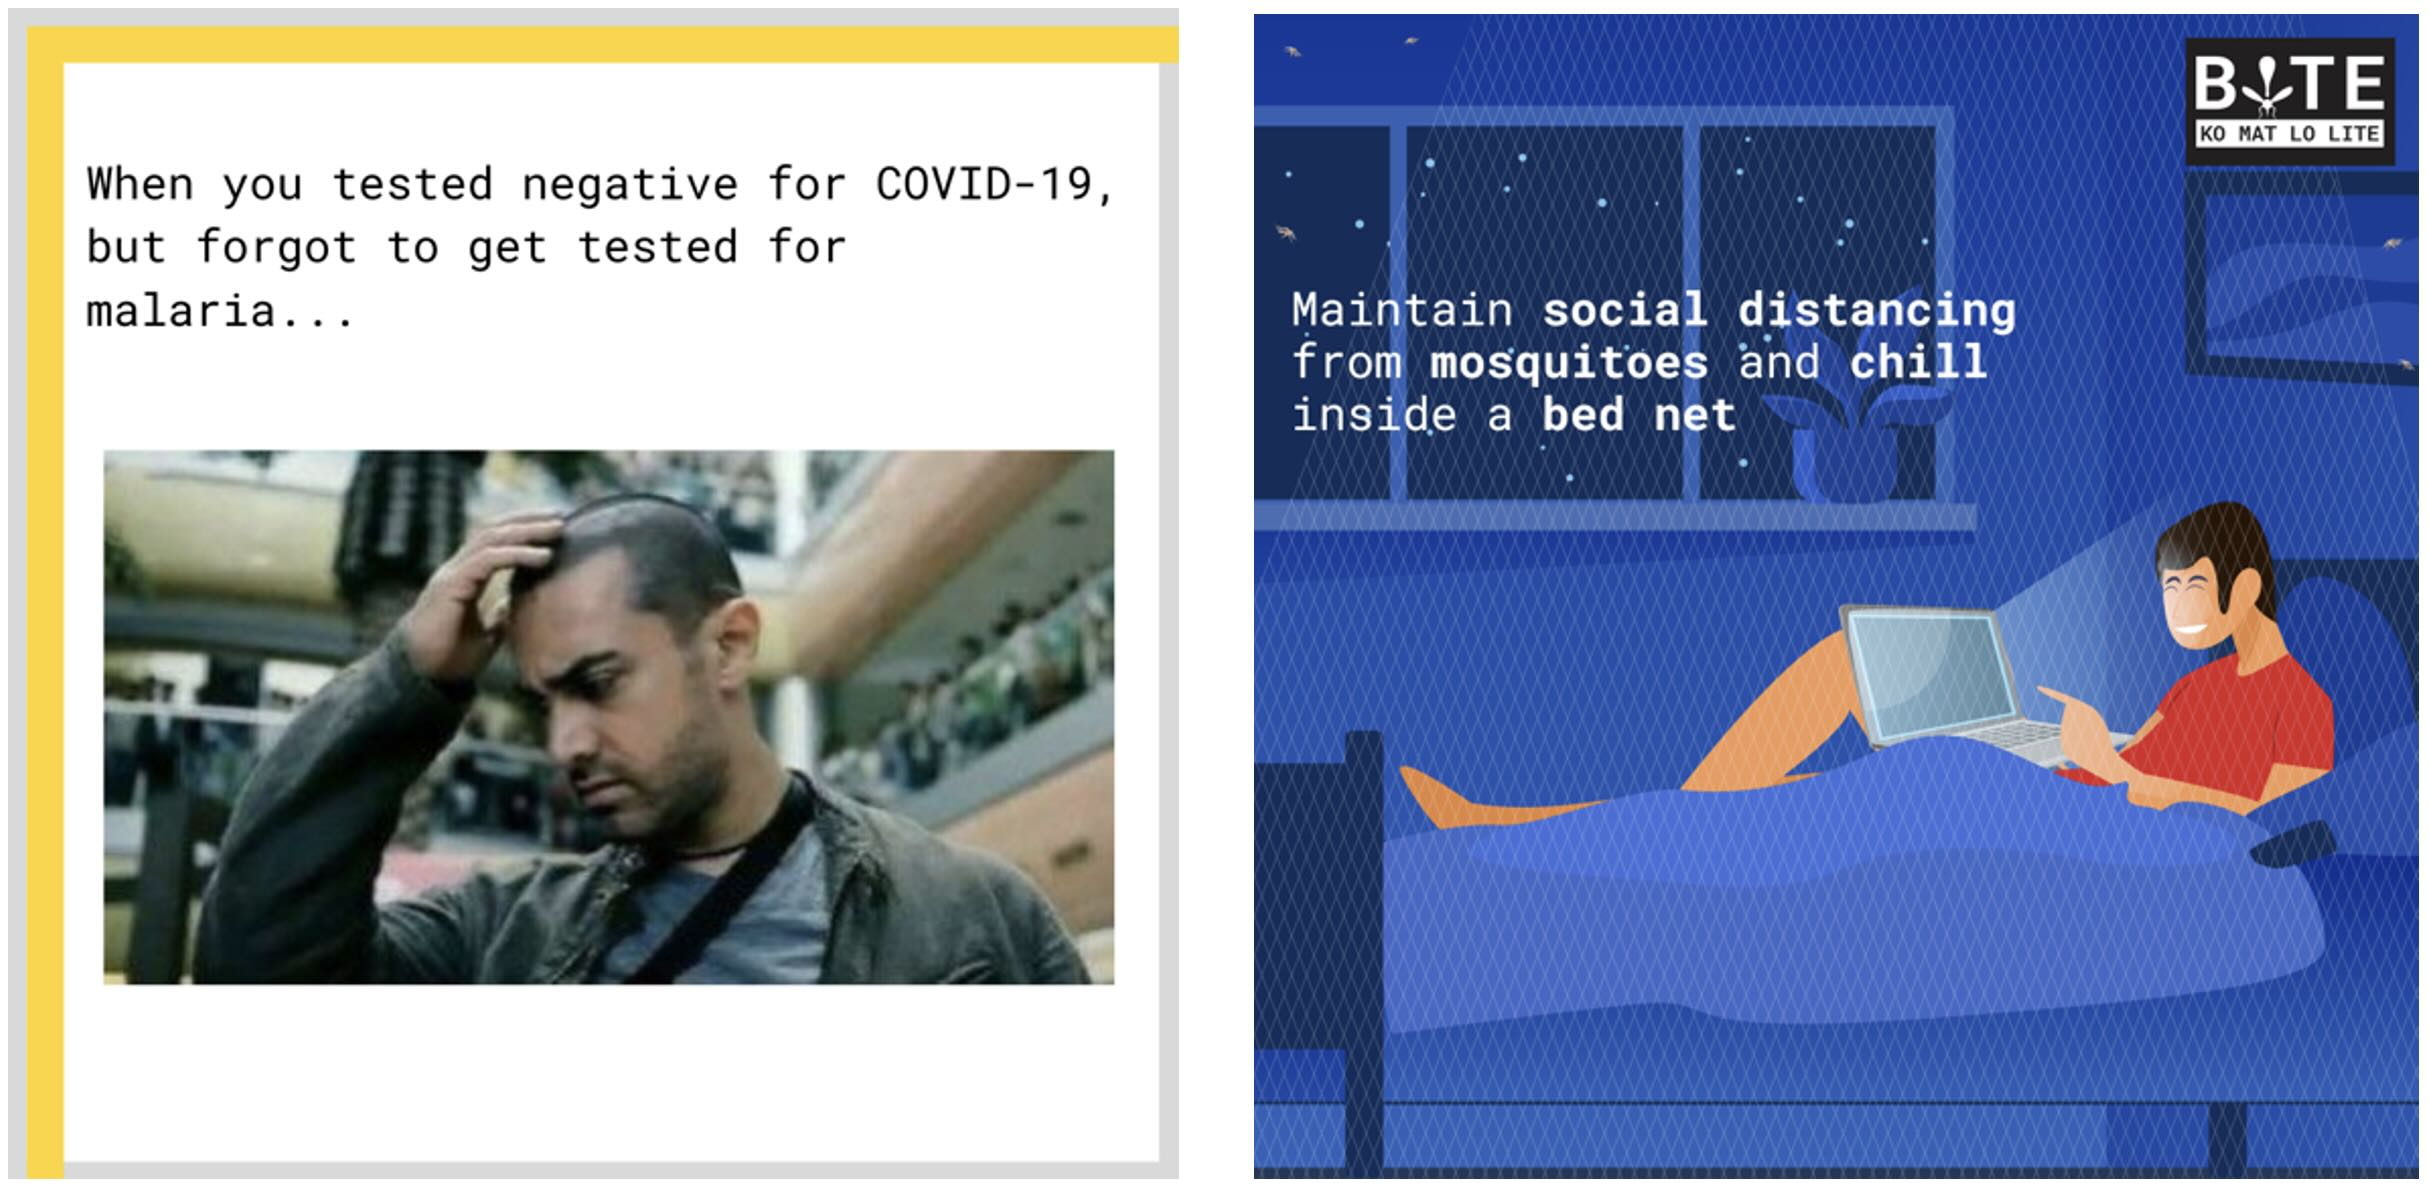
\includegraphics[width=13cm]{chapters/02-malaria/figures/Covid}
\end{figure}


\subsection{Campaign dissemination via Facebook and Instagram ads}
The dissemination of the content occurred in two phases (or campaigns). For the first campaign, from July to November in 2020, the MNM team used Meta Ad Manager to create one campaign with the objective of maximizing engagement. In that campaign, the team created six ad sets, each one targeting the demographic of a specific persona. The team limited the geographic targeting by excluding the treatment areas identified by the research team. The creative designed for each persona was placed in the appropriate ad set. Ads were turned off after they reached a frequency over five or noticed a significant drop in ad engagement. The team relied on the Meta Ad Algorithm to identify the highest-performing ad in each ad set. Figure \ref{fig:top_content} reports these ads.

During a second campaign in December 2020 and January 2021, the team used Meta Ad Manager to create one campaign also with the objective of maximizing engagement. In that campaign, the team created six ad sets, each one targeting the demographic of a specific persona. They then filled each ad set with the top-performing ad creatives from the first campaign.


\begin{figure}[h!]
	\centering
    \caption{Top performing content}
	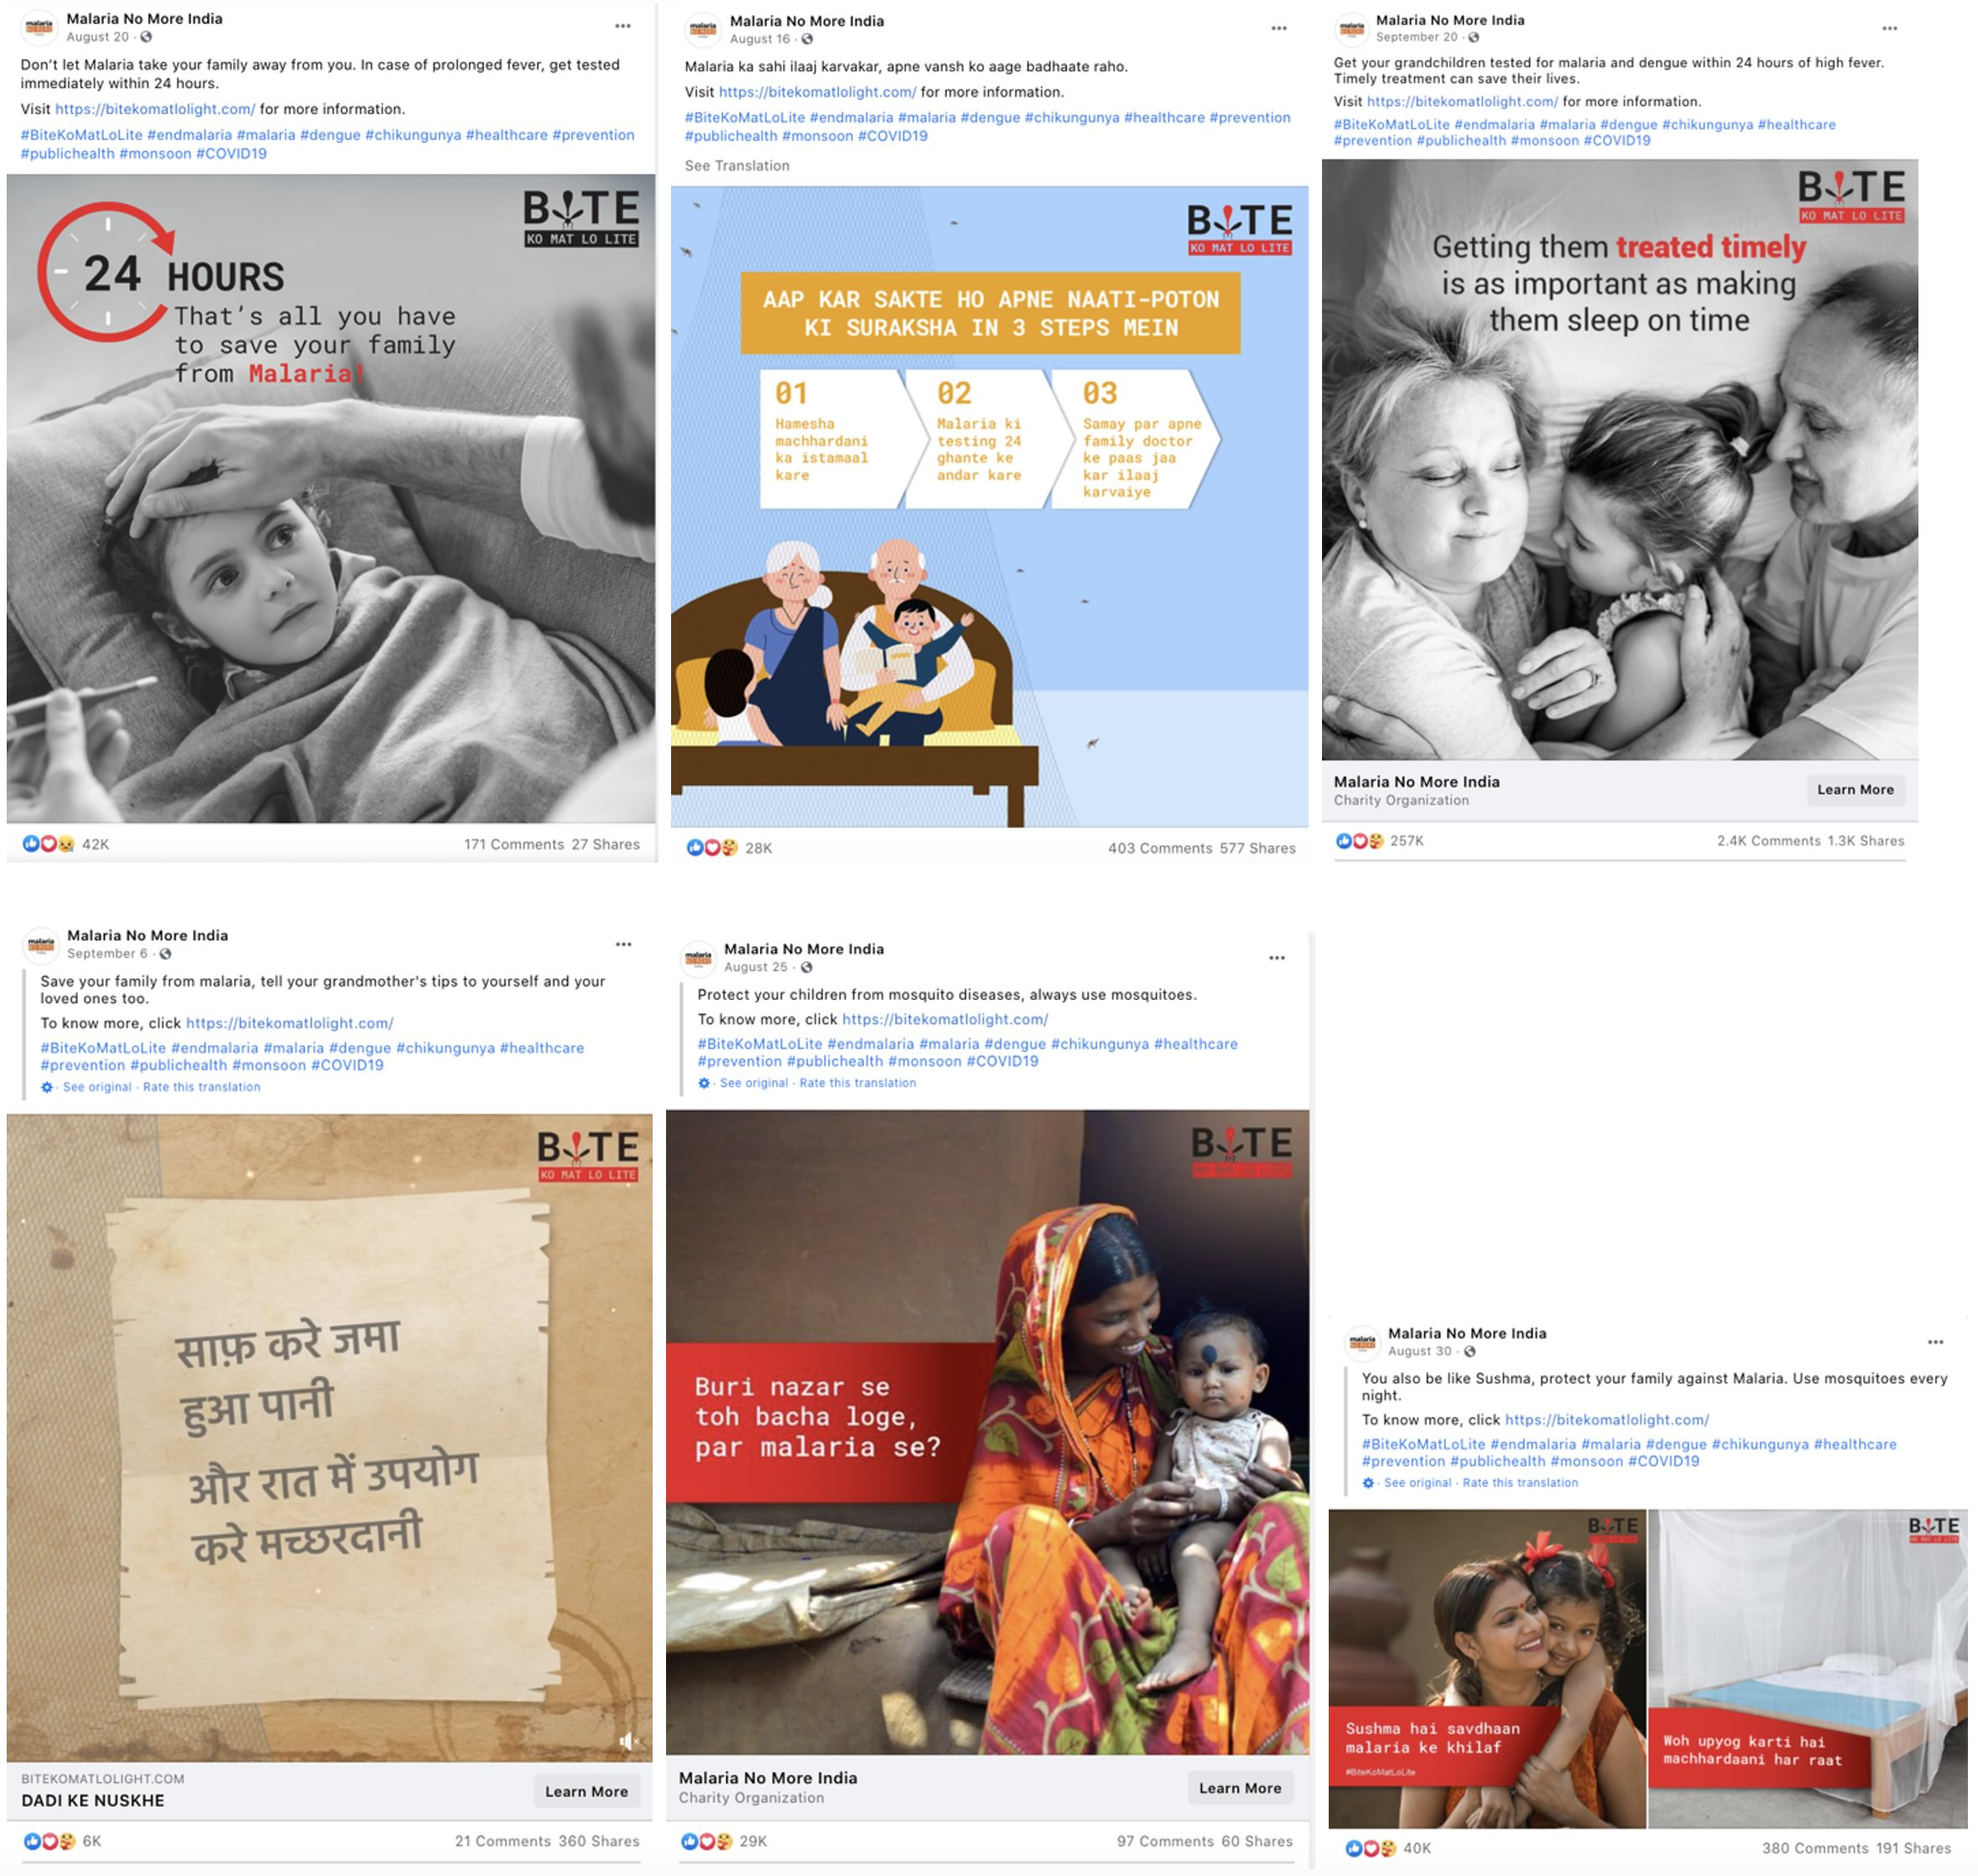
\includegraphics[scale=.38]{chapters/02-malaria/figures/TopPerforming}
 \label{fig:top_content}
\end{figure}



\subsection{Facebook and Instagram community management}
Instagram and Facebook channels require daily engagement. Malaria No More employed a community manager who oversaw comment threads across both channels. This person used a management guide equipped with pre-written responses for frequently asked questions. The following activities were carried out at least twice a day:
\begin{enumerate}
\item   Hiding all negative or nonconstructive (spam-like) comments \vspace{-0.1cm}
\item 	Liking all positive comments   \vspace{-0.1cm}
\item 	Responding to all Direct Messages \vspace{-0.1cm}
\item 	Inviting all the people who have engaged with the MNM page to also like the page \vspace{-0.1cm}
\end{enumerate}

\clearpage
\section{Data and Survey Questions}
\label{mal-appendix:B}
\setcounter{table}{0}
\renewcommand{\thetable}{B\arabic{table}}
\renewcommand{\theHtable}{B\arabic{table}} % for 'hyperref'


\subsection{Data Sources and Processing}

The data sources, cleaning steps, missing-covariate exclusions, and final analysis samples are reported in Table \ref{tab:data_cleaning} in the main text.




\subsection{Longitudinal Survey}
\setlist{nolistsep}
    \begin{itemize}[noitemsep]
    \item[a)] \textit{Did you sleep under a mosquito net last night?} This question was coded as 1 if the respondent reported to have slept under a bednet the previous night and 0 otherwise. Households without mosquito nets were excluded.
    \item[b)] \textit{How many family members that live in your house (including yourself) slept under a mosquito net last night?} This question required respondents to enter a number. We used this and family size to construct a new variable reflecting the share of family members who used a bednet the night before the interview. Households without mosquito nets were excluded.
    \item[c)] \textit{Thinking about yesterday, did you/your family use long-sleeve clothing to prevent mosquito bites?} and \textit{Thinking about yesterday, did you/ your family use body/wall sprays to prevent mosquito bites?} These two questions were coded as 1 if the respondent answered affirmatively, and 0 otherwise.
    \item[d)] \textit{Have you/someone in your family had a fever (100.4°F / 38°C or above) / malaria in the last two weeks?} This question was asked separately for fever and malaria, and was coded as 1 if the respondent answered affirmatively, and 0 otherwise.
    \item[e)] Conditional on respondent reporting a fever: \textit{Did you seek medical help?} This question was coded as 1 if answered affirmatively, and 0 otherwise. If yes: \textit{How long after the onset of the fever?} We coded as 1 those reporting help seeking within 24 hours.
    \item[f)] Conditional on respondent reporting malaria: \textit{Were you or your family members tested for Malaria?} This question was coded as 1 if answered affirmatively, and 0 otherwise. 
\end{itemize} 

\subsection{Cross-sectional Survey} 
\begin{itemize}[noitemsep]
    \item[a)] \textit{Have you/someone in your family had Malaria since last August?} This question was coded as 1 if answered affirmatively, and 0 otherwise.
  
    \item[b)] Conditional on respondent reporting malaria: \textit{How many family members (including yourself) have had Malaria since last August?} This question required respondents to enter a number. We used this and the family size to construct a new variable reflecting the share of family members who have had malaria since August 2020.

    \item[c)] \textit{How worried are you that you/someone in your family will get COVID-19/Malaria in the next year?} This question was asked separately for COVID-19 and malaria. Respondents could choose among four options, from ``Not at all worried" to ``Extremely worried''.

   \item[d)] \textit{Would you consider buying a mosquito net for your house?} This question was asked only to respondents without mosquito nets, and was coded as 1 if answered affirmatively, and 0 otherwise.
   
   \item[e)] \textit{Has your mosquito net been re-treated with an insecticide since last August?} This question was asked only to respondents with mosquito nets, and was coded as 1 if answered affirmatively, and 0 otherwise. 
\end{itemize}

\subsection{Individual-level Study} 
\begin{itemize}[noitemsep]
    \item[a)] \textit{Did you sleep under a mosquito net last night?} This question was coded as 1 if the
respondent reported to have slept under a bednet the previous night and 0 otherwise. Households without mosquito nets were excluded.

   \item[b)] \textit{What would you do if tomorrow you or a family member got a fever (100.4°F / 38°C or above) and there was a doctor or a healthcare facility near your home?} This question was coded as 1 if the respondent would seek treatment right away or within 24 hours of the onset of a fever.
  \end{itemize}

\newpage
\section{Figures}
\label{mal-appendix:C}

\setcounter{figure}{0}
\renewcommand{\thefigure}{\Alph{section}\arabic{figure}}
\renewcommand{\theHfigure}{\Alph{section}\arabic{figure}} % for 'hyperref'


\begin{figure}[h]
	\centering
    \caption{Potential reach of the MNM campaign}
	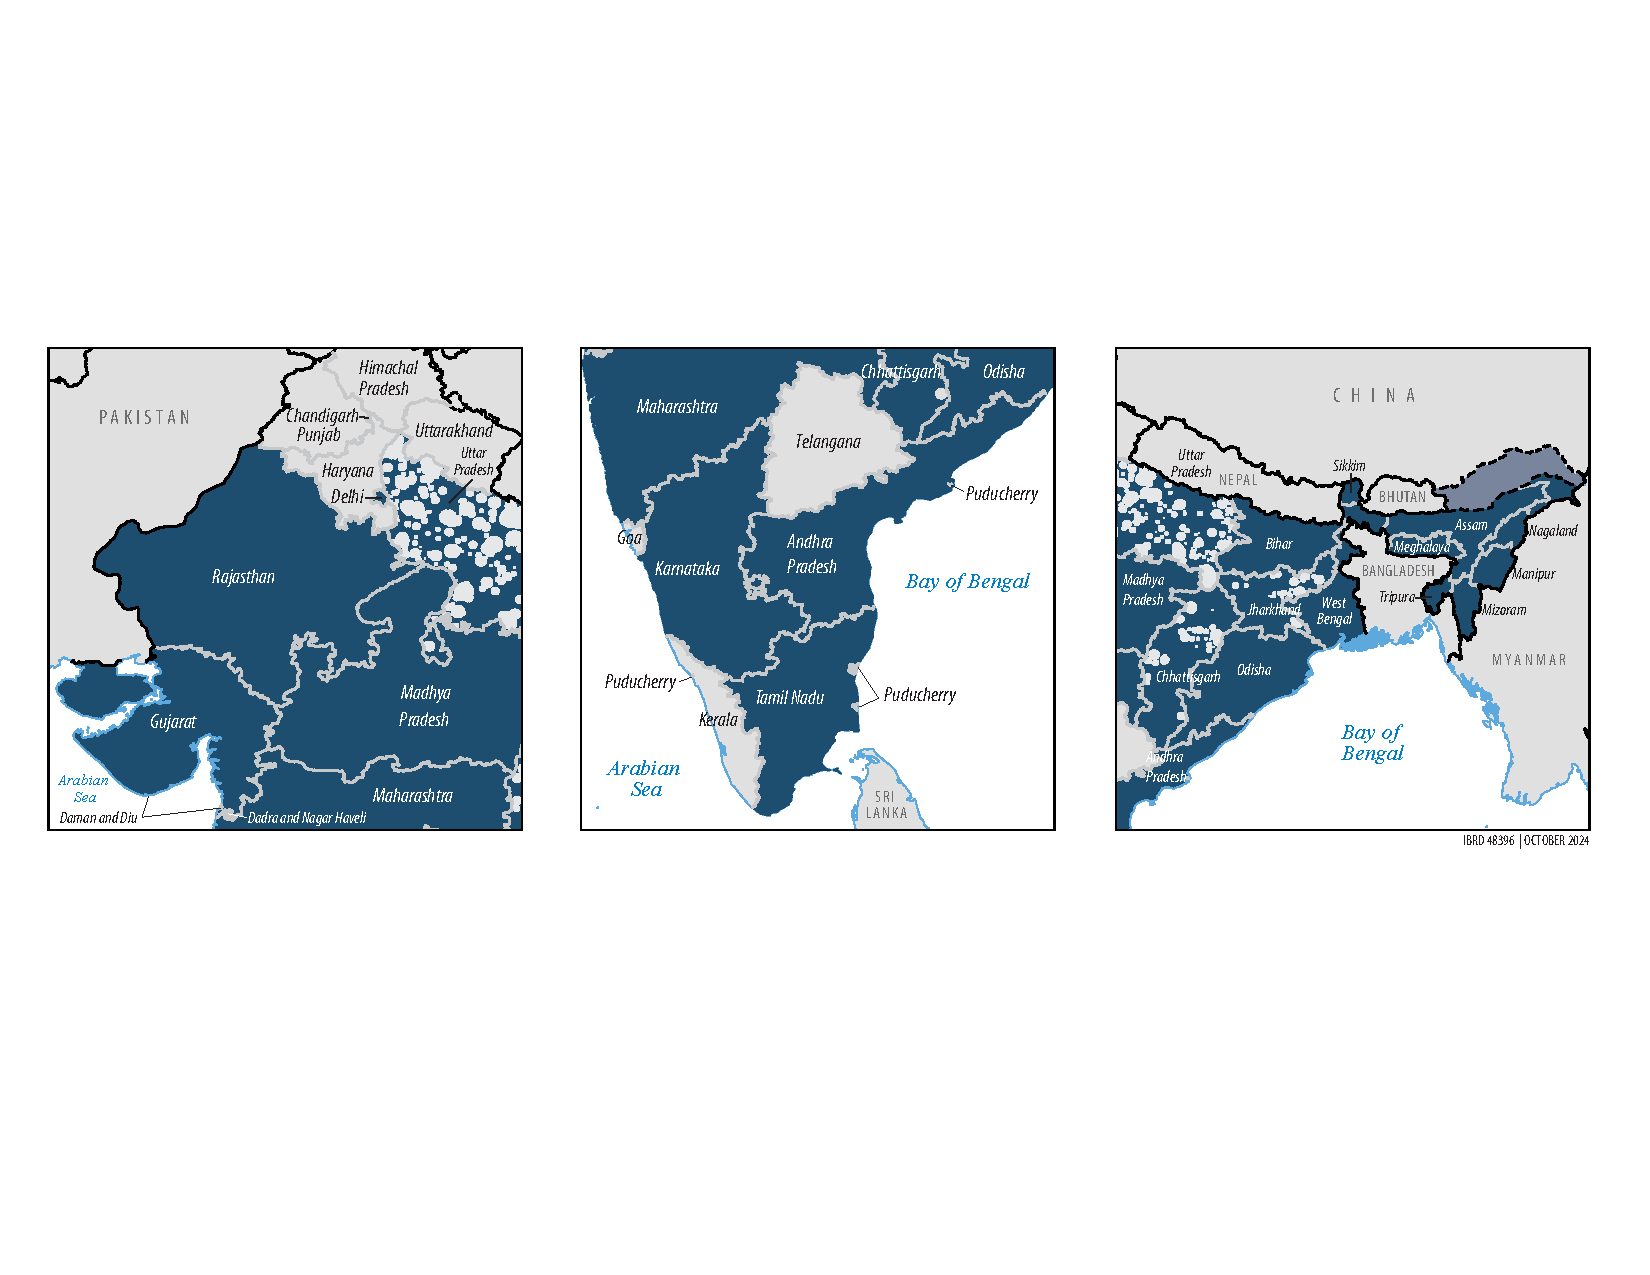
\includegraphics[scale=0.65]{chapters/02-malaria/figures/india_map_wb.pdf}
    \label{fig:campaign_states}
    \begin{minipage}{17cm}
    
\includegraphics[scale=1]{chapters/02-malaria/figures/disclaimer_wb.pdf} \scriptsize {This map was produced by the Cartography Unit of the World Bank Group. The boundaries, colors, denominations and any other information shown on this map do not imply, on the part of the World Bank Group, any judgment on the legal status of any territory, or any endorsement or acceptance of such boundaries. \\
    Notes: The MNM campaign targeted individuals residing in the 22 states in blue. These are: Manipur, Assam, Andhra Pradesh, Delhi, Gujarat, Maharashtra, Meghalaya, Karnataka, Nagaland, Odisha, Rajasthan, Tamil Nadu, Tripura, West Bengal, Sikkim, Arunachal Pradesh, Mizoram, Bihar, Madhya Pradesh, Uttar Pradesh, Chhattisgarh, Jharkhand. The last three states were part of the evaluation exercise and the gray circles in the map represent the control districts, which were excluded from the targeting of the campaign.}
\end{minipage}

\end{figure}



\begin{figure}[h]
	\centering
 \caption{Examples of Recruitment ads}
	
\includegraphics[scale=0.12]{chapters/02-malaria/figures/Ad1}
    
\includegraphics[scale=0.12]{chapters/02-malaria/figures/Ad2}
    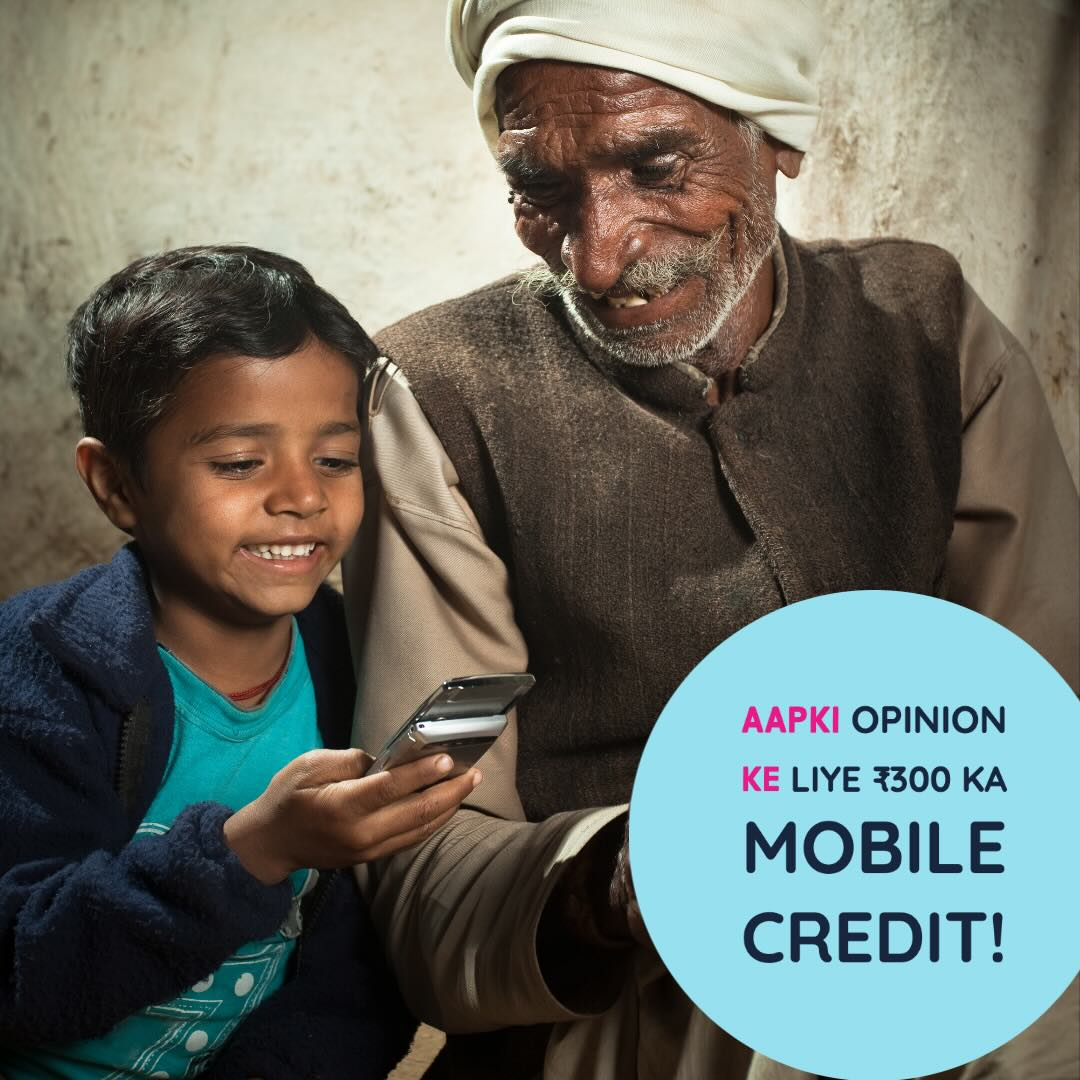
\includegraphics[scale=0.12]{chapters/02-malaria/figures/Ad3}	
    \label{fig:recruitment_ads}
\end{figure}

%\begin{figure}[h!]
%	\centering
%    \caption{Survey-sample optimization}
%	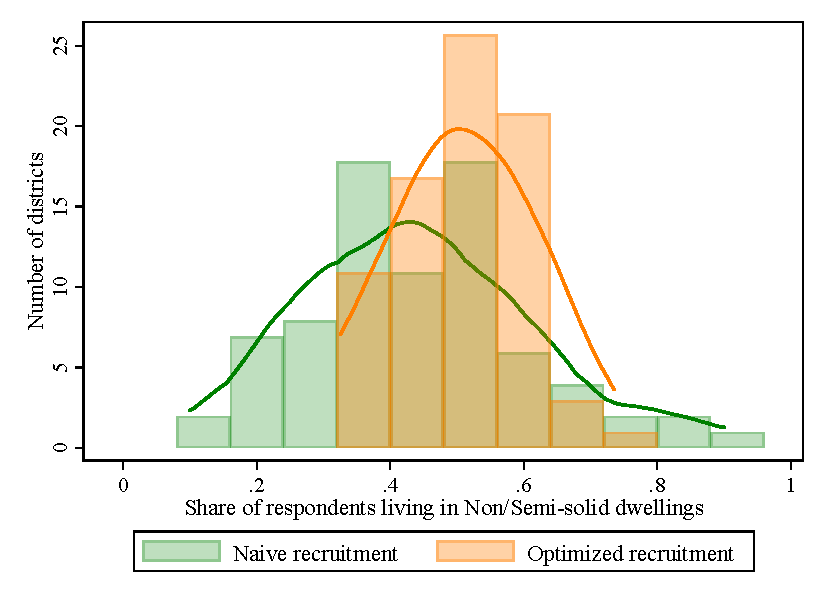
\includegraphics[scale=1]{chapters/02-malaria/figures/optimization.pdf}
%    \label{fig:recruitment}
%\end{figure}


\clearpage
\section{Tables}
\label{mal-appendix:D}
 \setcounter{table}{0}
\renewcommand{\thetable}{\Alph{section}\arabic{table}}
\renewcommand{\theHtable}{\Alph{section}\arabic{table}} % for 'hyperref'



\begin{table}[h!]
    \centering
    \caption{Comparison of district characteristics by study inclusion} 
     \footnotesize
    \adjustbox{max width=\textwidth}{%
\begin{tabular}{lccccc}
\hline  & In Study & Out of Study & Normalized & \it T-test & \\
 & \it Mean & \it Mean & Difference & (\it p-value) & \\
 & (1) & (2) & (3) & (4) & \\
\hline
\textbf{N. of districts} & 79 & 42 &  &  & \\ &  &  &  &  & \\[-5ex]\\
\textbf{A: Scoping survey (August 2020)} &  &  &  &  & \\
 &  &  &  &  & \\[-5ex]\\
Share living in solid houses & 0.498 & 0.386 & 0.507 & 0.000 & \\
Share with university degree & 0.596 & 0.578 & 0.079 & 0.495 & \\
Share unemployed & 0.443 & 0.450 & -0.031 & 0.787 & \\
Share with malaria in last 2 weeks & 0.016 & 0.019 & -0.096 & 0.437 & \\
Share with malaria in last 5 years & 0.187 & 0.230 & -0.231 & 0.072 & \\
Average cost per mille (USD) & 0.761 & 1.341 & -0.744 & 0.000 & \\
Average click-through rate (\%) & 1.838 & 1.566 & 0.799 & 0.000 & \\
Average ad cost per survey started (USD) & 0.247 & 1.031 & -0.957 & 0.000 & \\
Average ad cost per survey completed (USD) & 0.839 & 4.419 & -1.053 & 0.000 & \\
\hline \\[-5.1ex] &  &  &  &  & \\
 \textbf{B: Administrative sources (2011-2020)} &  &  &  &  & \\
 &  &  &  &  & \\[-5ex]\\
Area (thousand sq km) & 3.606 & 3.479 & 0.053 & 0.690 & \\
Population (millions, Census 2011) & 2.692 & 1.107 & 1.223 & 0.000 & \\
Population (millions, UN, 2020 estimate) & 2.941 & 1.211 & 1.173 & 0.000 & \\
Share of rural population (UN, 2020 estimate) & 0.710 & 0.873 & -0.772 & 0.000 & \\
Malaria positivity rate (Sep 2019 - Aug 2020) & 0.018 & 0.019 & -0.030 & 0.824 & \\
Household size & 5.827 & 5.342 & 0.531 & 0.001 & \\
Share of females & 0.479 & 0.489 & -0.592 & 0.000 & \\
Share of Hindu & 0.821 & 0.719 & 0.396 & 0.002 & \\
Share with age under 7 & 0.154 & 0.164 & -0.423 & 0.003 & \\
Socioeconomic Development Index & 0.364 & -0.899 & 1.046 & 0.000 & \\
Share from ST and SC/Dalit castes & 0.251 & 0.446 & -0.785 & 0.000 & \\
Share unemployed & 0.649 & 0.567 & 0.905 & 0.000 & \\
Share with no literacy & 0.422 & 0.482 & -0.549 & 0.000 & \\
Share living in solid houses & 0.586 & 0.321 & 0.967 & 0.000 & \\
Share living in semi-solid houses & 0.254 & 0.535 & -0.900 & 0.000 & \\
Share with banking access & 0.672 & 0.534 & 0.692 & 0.000 & \\
Share with radio & 0.215 & 0.179 & 0.359 & 0.022 & \\
Share with tv & 0.326 & 0.171 & 0.934 & 0.000 & \\
Share with bicycle & 0.649 & 0.613 & 0.208 & 0.138 & \\
Share with motorbike & 0.185 & 0.109 & 0.976 & 0.000 & \\
Share with car & 0.034 & 0.016 & 0.576 & 0.001 & \\
Share with mobile phone & 0.563 & 0.376 & 0.812 & 0.000 & \\
Share with landline phone & 0.030 & 0.016 & 0.897 & 0.000 & \\
Share with internet & 0.016 & 0.005 & 0.483 & 0.007 & \\
\hline \\[-5.1ex] &  &  &  &  & \\
 \textbf{C: Demographic and Health Survey (2019-2021)} &  &  &  &  & \\
 &  &  &  &  & \\[-5ex]\\
Share from disadvantaged castes       &           0.808  &     0.896    &    -0.805    &    0.000 & \\
Share with no education & 0.322 & 0.398 & -0.614 & 0.000 & \\
Share with closed drainage system & 0.381 & 0.176 & 0.935 & 0.000 & \\
Share covered by health insurance & 0.255 & 0.521 & -0.842 & 0.000 & \\
Share with access to public health facility & 0.666 & 0.788 & -0.790 & 0.000 & \\
Number of bednets in the household & 1.023 & 1.320 & -0.421 & 0.002 & \\
Share with mobile phone & 0.937 & 0.876 & 0.717 & 0.000 & \\
Share with internet & 0.524 & 0.417 & 0.701 & 0.000 & \\
 \hline \hline \\[-5.1ex] &  &  &  &  & \\
\multicolumn{5}{p{.95\linewidth}}{\scriptsize Notes: The table reports district characteristics from the scoping survey (Panel A) and administrative sources (Panel B), and the India Demographic and Health Survey (Panel C), comparing districts included in the study to those excluded. Administrative data refer to the 2011 Census unless otherwise specified. The normalized difference is calculated as the difference in means divided by the square root of the sum of the two variances.}
\end{tabular}
}%
\\
    \label{tab:districts_characteristics_bystudy}
\end{table}


\begin{table}[h!]
    \centering
    \caption{Household-level predictors of malaria incidence}
    \footnotesize
    %\hspace*{-1cm}
    {
\def\sym#1{\ifmmode^{#1}\else\(^{#1}\)\fi}
\adjustbox{max width=\textwidth}{%
\begin{tabular}{l*{4}{c}}
\hline\hline
                &\multicolumn{2}{c}{\begin{tabular}{@{}c@{}}Any HH member had malaria\\in last 5 years\end{tabular}}&\multicolumn{2}{c}{\begin{tabular}{@{}c@{}}Any HH member had malaria\\in last 2 weeks\end{tabular}}\\\cmidrule(lr){2-3}\cmidrule(lr){4-5}
                &\multicolumn{1}{c}{(1)}         &\multicolumn{1}{c}{(2)}         &\multicolumn{1}{c}{(3)}         &\multicolumn{1}{c}{(4)}         \\
\hline
Solid house     &   -0.025\sym{***}&                  &   -0.006\sym{***}&                  \\
                &  (0.007)         &                  &  (0.002)         &                  \\
Semi-solid house&   -0.005         &                  &   -0.004\sym{*}  &                  \\
                &  (0.007)         &                  &  (0.002)         &                  \\
Within 60 min to health facility&   -0.010\sym{**} &                  &   -0.003         &                  \\
                &  (0.005)         &                  &  (0.002)         &                  \\
University degree&    0.023\sym{***}&                  &    0.001         &                  \\
                &  (0.005)         &                  &  (0.002)         &                  \\
Advantaged caste&   -0.013\sym{***}&                  &   -0.003\sym{**} &                  \\
                &  (0.004)         &                  &  (0.001)         &                  \\
Has air conditioning&   -0.006         &                  &    0.001         &                  \\
                &  (0.005)         &                  &  (0.001)         &                  \\
Household size  &    0.017\sym{***}&                  &    0.005\sym{**} &                  \\
                &  (0.005)         &                  &  (0.002)         &                  \\
SES index (PC1 score)&                  &   -0.022\sym{***}&                  &   -0.004\sym{***}\\
                &                  &  (0.004)         &                  &  (0.001)         \\
Constant        &    0.184\sym{***}&    0.184\sym{***}&    0.016\sym{***}&    0.016\sym{***}\\
                &  (0.011)         &  (0.011)         &  (0.001)         &  (0.001)         \\
\hline
Observations    &\num{7548}         &\num{7548}         &\num{7548}         &\num{7548}         \\
Adj. R-squared  &    0.010         &    0.003         &    0.004         &    0.001         \\
Mean of Y       &    0.184         &    0.184         &    0.016         &    0.016         \\
\hline\hline
\multicolumn{5}{p{.87\linewidth}}{\scriptsize Notes: Columns (1)-(3) report OLS coefficients from multivariate regressions of malaria incidence on standardized SES components. Columns (2)-(4)  report regressions of malaria incidence on the SES index (PC1 score) only. Baseline responses collected from July 23 to August 19, 2020 are included in the sample. Standard errors are clustered at the district level. \sym{*} \(p<0.1\), \sym{**} \(p<0.05\), \sym{***} \(p<0.01\).}\\
\end{tabular}
}%

}

    \label{tab:malaria_predictors}
\end{table}

\begin{table}[h!]
    \centering
    \caption{Additional district characteristics by experimental condition (2011 Census)} 
     \footnotesize
    \adjustbox{max width=\textwidth}{%
\begin{tabular}{lccccc}
\hline  & Treatment & Control & Normalized & \it T-test & \\
 & \it Mean & \it Mean & Difference & (\it p-value) & \\
 & (1) & (2) & (3) & (4) & \\
\hline
N. of districts & 39 & 40 &  &  & \\
Share from ST and SC/Dalit castes & 0.245 & 0.256 & -0.072 & 0.652 & \\
Share unemployed & 0.648 & 0.650 & -0.026 & 0.872 & \\
Share with no literacy & 0.430 & 0.415 & 0.166 & 0.299 & \\
Share living in solid houses & 0.602 & 0.570 & 0.120 & 0.453 & \\
Share living in semi-solid houses & 0.257 & 0.252 & 0.015 & 0.926 & \\
Share of urban living in solid houses & 0.791 & 0.782 & 0.071 & 0.656 & \\
Share of rural living in solid houses & 0.542 & 0.519 & 0.076 & 0.635 & \\
Share of urban living in semi-solid houses & 0.138 & 0.134 & 0.027 & 0.868 & \\
Share of rural living in semi-solid houses & 0.298 & 0.285 & 0.041 & 0.798 & \\
Share with banking access & 0.668 & 0.676 & -0.046 & 0.774 & \\
Share with radio & 0.211 & 0.220 & -0.082 & 0.606 & \\
Share with tv & 0.338 & 0.315 & 0.111 & 0.489 & \\
Share with bicycle & 0.626 & 0.672 & -0.314 & 0.052 & \\
Share with motorbike & 0.194 & 0.177 & 0.177 & 0.268 & \\
Share with car & 0.039 & 0.029 & 0.229 & 0.151 & \\
Share with mobile phone & 0.567 & 0.558 & 0.047 & 0.770 & \\
Share with landline phone & 0.031 & 0.029 & 0.140 & 0.380 & \\
Share with internet & 0.019 & 0.013 & 0.219 & 0.170 & \\
\hline \hline  \\[-5.1ex] &  &  &  &  & \\
\multicolumn{5}{p{.85\linewidth}}{\scriptsize Notes: The table reports district characteristics by experimental condition. All data are from the 2011 Census. The normalized difference is calculated as the difference in means divided by the square root of the sum of the two variances.}
\end{tabular}
}%
\\

    \label{tab:districts_census_extra_balance}
\end{table}

\begin{table}[h!]
    \centering
    \caption{Longitudinal Sample - Baseline covariates and outcomes by experimental condition} 
     \footnotesize
    \adjustbox{max width=\textwidth}{%
\begin{tabular}{lccccc}
\hline  & Treatment & Control & Normalized & \it T-test & \\
 & \it Mean & \it Mean & Difference & (\it p-value) & \\
 & (1) & (2) & (3) & (4) & \\
\hline \hline \textbf{Panel A: Covariates} &  &  &  &  & \\
 &  &  &  &  & \\[-5ex]\\
N. of respondents & 2524 & 2677 &  &  & \\
N. of total survey waves per respondent & 3.031 & 2.991 & 0.013 & 0.700 & \\
Female & 0.084 & 0.088 & -0.011 & 0.628 & \\
N. of HH members & 6.540 & 6.700 & -0.032 & 0.316 & \\
Solid house & 0.469 & 0.455 & 0.020 & 0.517 & \\
Non/Semi-solid house & 0.531 & 0.545 & -0.020 & 0.517 & \\
Age & 27.266 & 26.980 & 0.024 & 0.382 & \\
Has completed university & 0.594 & 0.598 & -0.005 & 0.854 & \\
Has completed secondary school & 0.273 & 0.266 & 0.011 & 0.665 & \\
Has completed primary school & 0.097 & 0.102 & -0.013 & 0.577 & \\
Unemployed & 0.485 & 0.501 & -0.024 & 0.267 & \\
Student & 0.195 & 0.181 & 0.025 & 0.245 & \\
OBC caste & 0.372 & 0.390 & -0.026 & 0.324 & \\
SC/Dalit caste & 0.121 & 0.130 & -0.019 & 0.456 & \\
ST caste & 0.064 & 0.052 & 0.036 & 0.505 & \\
General caste & 0.399 & 0.385 & 0.021 & 0.513 & \\
Medical center distance < 15min & 0.275 & 0.270 & 0.007 & 0.798 & \\
Medical center distance 15-30min & 0.266 & 0.267 & -0.001 & 0.973 & \\
Medical center distance 30-60min & 0.211 & 0.216 & -0.010 & 0.663 & \\
Has mosquito net & 0.761 & 0.778 & -0.027 & 0.530 & \\
Has air conditioning & 0.091 & 0.076 & 0.038 & 0.117 & \\
Pregnant woman in house & 0.133 & 0.128 & 0.010 & 0.675 & \\
Hindu & 0.843 & 0.865 & -0.045 & 0.234 & \\
Muslim & 0.116 & 0.099 & 0.038 & 0.378 & \\
Any member had malaria in last 5 years & 0.206 & 0.209 & -0.004 & 0.925 & \\
Worried/Very worried about malaria & 0.357 & 0.370 & -0.019 & 0.315 & \\
Worried/Very worried about COVID-19 & 0.449 & 0.448 & 0.001 & 0.970 & \\
\hline \hline \\[-5.5ex] &  &  &  &  & \\
\textbf{Panel B: Outcomes} &  &  &  &  & \\
 &  &  &  &  & \\[-5ex]\\
Used bednet the previous night & 0.710 & 0.694 & 0.024 & 0.512 & \\
Share of HH members who used bednet the previous night & 0.708 & 0.685 & 0.045 & 0.220 & \\
Used long-sleeve clothing the previous day & 0.561 & 0.582 & -0.029 & 0.384 & \\
Used body/wall sprays the previous day & 0.351 & 0.369 & -0.027 & 0.292 & \\
Any member had malaria in last 2 weeks & 0.019 & 0.019 & -0.000 & 0.988 & \\
Any member had a fever in last 2 weeks & 0.063 & 0.067 & -0.011 & 0.658 & \\
Any member tested for malaria & 0.596 & 0.580 & 0.022 & 0.873 & \\
Any member sought medical help if fever & 0.792 & 0.849 & -0.105 & 0.224 & \\
\hline \\[-5.1ex] &  &  &  &  & \\
\hline\end{tabular}
}%
\\
\begin{minipage}{1\linewidth}
  \scriptsize  The table reports covariates and outcomes measured at baseline for individuals' and households' in the experience sample, by experimental condition. The normalized difference is the difference between the two means divided by the square root of the sum of the variances of the two variables.\\
\end{minipage}


    \label{tab:panel_sample_balance}
\end{table}


\begin{table}[h!]
    \centering
    \caption{Cross-sectional Sample - Covariates by experimental condition} 
     \footnotesize
    \adjustbox{max width=\textwidth}{%
\begin{tabular}{lccccc}
\hline  & Treatment & Control & Normalized & \it T-test & \\
 & \it Mean & \it Mean & Difference & (\it p-value) & \\
 & (1) & (2) & (3) & (4) & \\
\hline \hline \textbf{Covariates} &  &  &  &  & \\
 &  &  &  &  & \\[-5ex]\\
N. of respondents & 1476 & 1576 &  &  & \\
Female & 0.121 & 0.115 & 0.013 & 0.669 & \\
N. of HH members & 6.524 & 6.442 & 0.016 & 0.668 & \\
Solid house & 0.425 & 0.437 & -0.016 & 0.633 & \\
Non/Semi-solid house & 0.575 & 0.563 & 0.016 & 0.633 & \\
Age & 27.238 & 27.699 & -0.034 & 0.300 & \\
Has completed university & 0.566 & 0.560 & 0.009 & 0.798 & \\
Has completed secondary school & 0.255 & 0.278 & -0.036 & 0.195 & \\
Has completed primary school & 0.121 & 0.114 & 0.015 & 0.505 & \\
Unemployed & 0.545 & 0.496 & 0.071 & 0.008 & \\
Student & 0.180 & 0.201 & -0.037 & 0.204 & \\
OBC caste & 0.341 & 0.345 & -0.006 & 0.869 & \\
SC/Dalit caste & 0.122 & 0.121 & 0.002 & 0.955 & \\
ST caste & 0.060 & 0.055 & 0.015 & 0.715 & \\
General caste & 0.438 & 0.438 & -0.000 & 0.995 & \\
Medical center distance < 15min & 0.307 & 0.280 & 0.041 & 0.132 & \\
Medical center distance 15-30min & 0.280 & 0.282 & -0.002 & 0.934 & \\
Medical center distance 30-60min & 0.192 & 0.199 & -0.013 & 0.589 & \\
Has mosquito net & 0.701 & 0.711 & -0.016 & 0.763 & \\
Mosquito nets per HH member & 0.499 & 0.511 & -0.015 & 0.739 & \\
Has air conditioning & 0.100 & 0.096 & 0.007 & 0.788 & \\
Pregnant woman in house & 0.158 & 0.133 & 0.049 & 0.085 & \\
Hindu & 0.862 & 0.865 & -0.005 & 0.902 & \\
Muslim & 0.102 & 0.101 & 0.003 & 0.937 & \\
\hline \\[-5.1ex] &  &  &  &  & \\
\hline\end{tabular}
}%
\\
\begin{minipage}{1\linewidth}
\scriptsize  The table reports  covariates for individuals' and households' in the cross-sectional sample by experimental condition. The normalized difference is the difference between the two means divided by the square root of the sum of the variances of the two variables.\\
\end{minipage}


    \label{tab:cross_section_balance}
\end{table}


\begin{table}[h!]
    \centering
    \caption{Longitudinal Sample 5+ waves - Baseline covariates/outcomes by experimental condition} 
     \footnotesize
    \adjustbox{max width=\textwidth}{%
\begin{tabular}{lccccc}
\hline  & Treatment & Control & Normalized & \it T-test & \\
 & \it Mean & \it Mean & Difference & (\it p-value) & \\
 & (1) & (2) & (3) & (4) & \\
\hline \hline \textbf{Panel A: Covariates} &  &  &  &  & \\
 &  &  &  &  & \\[-5ex]\\
N. of respondents & 704 & 744 &  &  & \\
N. of total survey waves per respondent & 5.947 & 5.961 & -0.012 & 0.752 & \\
Female & 0.064 & 0.074 & -0.028 & 0.456 & \\
N. of HH members & 6.321 & 6.526 & -0.042 & 0.352 & \\
Solid house & 0.520 & 0.491 & 0.041 & 0.346 & \\
Non/Semi-solid house & 0.480 & 0.509 & -0.041 & 0.346 & \\
Age & 27.562 & 27.171 & 0.035 & 0.364 & \\
Has completed university & 0.658 & 0.659 & -0.001 & 0.969 & \\
Has completed secondary school & 0.283 & 0.259 & 0.037 & 0.302 & \\
Has completed primary school & 0.045 & 0.070 & -0.074 & 0.059 & \\
Unemployed & 0.489 & 0.501 & -0.018 & 0.581 & \\
Student & 0.185 & 0.195 & -0.018 & 0.653 & \\
OBC caste & 0.381 & 0.398 & -0.025 & 0.603 & \\
SC/Dalit caste & 0.119 & 0.137 & -0.038 & 0.344 & \\
ST caste & 0.068 & 0.048 & 0.060 & 0.324 & \\
General caste & 0.402 & 0.383 & 0.027 & 0.563 & \\
Medical center distance < 15min & 0.281 & 0.263 & 0.028 & 0.542 & \\
Medical center distance 15-30min & 0.256 & 0.265 & -0.015 & 0.709 & \\
Medical center distance 30-60min & 0.186 & 0.227 & -0.072 & 0.065 & \\
Has mosquito net & 0.794 & 0.802 & -0.015 & 0.797 & \\
Has air conditioning & 0.085 & 0.073 & 0.033 & 0.390 & \\
Pregnant woman in house & 0.105 & 0.101 & 0.010 & 0.788 & \\
Hindu & 0.848 & 0.864 & -0.033 & 0.493 & \\
Muslim & 0.111 & 0.102 & 0.020 & 0.702 & \\
Any member had malaria in last 5 years & 0.224 & 0.214 & 0.018 & 0.782 & \\
Worried/Very worried about malaria & 0.342 & 0.347 & -0.007 & 0.845 & \\
Worried/Very worried about COVID-19 & 0.484 & 0.454 & 0.043 & 0.300 & \\
\hline \hline \\[-5.5ex] &  &  &  &  & \\
\textbf{Panel B: Outcomes} &  &  &  &  & \\
 &  &  &  &  & \\[-5ex]\\
Used bednet the previous night & 0.710 & 0.683 & 0.041 & 0.427 & \\
Share of HH members who used bednet the previous night & 0.713 & 0.690 & 0.044 & 0.386 & \\
Used long-sleeve clothing the previous day & 0.571 & 0.593 & -0.031 & 0.530 & \\
Used body/wall sprays the previous day & 0.352 & 0.364 & -0.018 & 0.648 & \\
Any member had malaria in last 2 weeks & 0.009 & 0.015 & -0.041 & 0.292 & \\
Any member had a fever in last 2 weeks & 0.053 & 0.069 & -0.047 & 0.231 & \\
Any member tested for malaria & 0.667 & 0.545 & 0.165 & 0.665 & \\
Any member sought medical help if fever & 0.838 & 0.843 & -0.010 & 0.955 & \\
\hline \\[-5.1ex] &  &  &  &  & \\
\hline\end{tabular}
}%
\\
\begin{minipage}{1\linewidth}
  \scriptsize  The table reports covariates and outcomes measured at baseline for individuals' and households' in the experience sample, by experimental condition. Only individuals who completed five or more survey waves are included. The normalized difference is the difference between the two means divided by the square root of the sum of the variances of the two variables.\\
\end{minipage}


    \label{tab:panel_sample_balance_attrition}
\end{table}



\begin{table}[h!]
    \centering
    \caption{Longitudinal Sample: Differential Attrition Analysis} 
     \footnotesize
    {
\def\sym#1{\ifmmode^{#1}\else\(^{#1}\)\fi}
\adjustbox{max width=\textwidth}{%
\begin{tabular}{l*{2}{c}}
\hline\hline
                &\multicolumn{2}{c}{Y=1 if individual response is missing in eligible survey wave}\\\cmidrule(lr){2-3}
                &\multicolumn{1}{c}{(1)}         &\multicolumn{1}{c}{(2)}         \\
                &   T only         &T + T $\times$ Wave         \\
\hline
T               &   -0.005         &    0.019         \\
                &  (0.011)         &  (0.017)         \\
T $\times$ Wave 2&                  &   -0.047         \\
                &                  &  (0.041)         \\
T $\times$ Wave 3&                  &   -0.031         \\
                &                  &  (0.033)         \\
T $\times$ Wave 4&                  &   -0.027         \\
                &                  &  (0.030)         \\
T $\times$ Wave 5&                  &   -0.029         \\
                &                  &  (0.028)         \\
T $\times$ Wave 6&                  &   -0.022         \\
                &                  &  (0.027)         \\
T $\times$ Wave 7&                  &   -0.023         \\
                &                  &  (0.027)         \\
T $\times$ Wave 8&                  &   -0.022         \\
                &                  &  (0.023)         \\
T $\times$ Wave 9&                  &   -0.022         \\
                &                  &  (0.017)         \\
Wave FE         &\(\checkmark\)         &\(\checkmark\)         \\
\hline
Observations    &\num{57685}         &\num{57685}         \\
Adj. R-squared  &    0.230         &    0.230         \\
\hline\hline
\multicolumn{3}{p{.75\linewidth}}{\scriptsize Notes: The table reports estimates from individual-wave regressions in which the dependent variable equals one if the respondent did not answer a given eligible post-treatment survey wave in the raw data, and zero otherwise. \(T\) is the treatment indicator.  Column (1) includes the treatment indicator and wave fixed effects. Column (2) additionally includes interactions between the treatment indicator and wave dummies. State fixed effects are included in all columns. Standard errors are clustered at the district level. \sym{*} \(p<0.1\), \sym{**} \(p<0.05\), \sym{***} \(p<0.01\)}\\
\end{tabular}
}%

}

    \label{tab:panel_attrition_by_arm}
\end{table}







\begin{table}[h!]
    \centering
    \caption{Baseline subdistrict characteristics by experimental condition} 
     \footnotesize
    \adjustbox{max width=\textwidth}{%
\begin{tabular}{lccccc}
\hline  & Treatment & Control & Normalized & \it T-test & \\
 & \it Mean & \it Mean & Difference & (\it p-value) & \\
 & (1) & (2) & (3) & (4) & \\
\hline 
N. of subdistricts & 62 & 57 &  &  & \\
Population (millions, UN, 2020 estimate) & 0.737 & 0.654 & 0.103 & 0.427 & \\
Share of rural population (UN, 2020 estimate) & 0.671 & 0.712 & -0.125 & 0.336 & \\
Area (thousand sq km) & 0.060 & 0.067 & -0.128 & 0.320 & \\
Elevation mean (m) & 201.598 & 204.015 & -0.016 & 0.905 & \\
Elevation std. deviation (m) & 11.480 & 13.916 & -0.095 & 0.462 & \\
Distance to district capital (thousand km) & 2.021 & 1.731 & 0.206 & 0.112 & \\
Malaria tests conducted per thousand people & 2.489 & 3.754 & -0.131 & 0.312 & \\
Urban malaria positivity rate (\%) & 2.175 & 0.978 & 0.165 & 0.385 & \\
Rural malaria positivity rate (\%) & 2.666 & 0.621 & 0.153 & 0.273 & \\
\hline \\[-5.1ex] &  &  &  &  & \\
\hline
\multicolumn{5}{p{.9\linewidth}}{\scriptsize Notes: The table reports subdistrict characteristics before the campaign, by experimental condition. Only subdistricts with more than 50\% of the population within study circles are included. The normalized difference is the difference between the two means divided by the square root of the sum of the variances of the two variables.}
\end{tabular}
}%
\\
    \label{tab:subdistricts_balance}
\end{table}





\begin{table}[h!]
    \centering
    \caption{Concerns about malaria, bednet ownership, willingness to purchase, and knowledge (after the campaign) }
        \begin{minipage}{16cm}
\end{minipage}
    \footnotesize
    %\hspace*{-1cm}
    {
\def\sym#1{\ifmmode^{#1}\else\(^{#1}\)\fi}
\adjustbox{max width=\textwidth}{%
\begin{tabular}{l*{8}{c}}
\hline\hline
                &\multicolumn{2}{c}{\shortstack{Respondent is very\\ worried about malaria}}&\multicolumn{2}{c}{\shortstack{Respondent\\has a bednet}}&\multicolumn{2}{c}{\shortstack{Respondent\\would buy bednet}}&\multicolumn{2}{c}{\shortstack{Respondent knows \\ where to buy bednet}}\\\cmidrule(lr){2-3}\cmidrule(lr){4-5}\cmidrule(lr){6-7}\cmidrule(lr){8-9}
                &\multicolumn{1}{c}{(1)}         &\multicolumn{1}{c}{(2)}         &\multicolumn{1}{c}{(3)}         &\multicolumn{1}{c}{(4)}         &\multicolumn{1}{c}{(5)}         &\multicolumn{1}{c}{(6)}         &\multicolumn{1}{c}{(7)}         &\multicolumn{1}{c}{(8)}         \\
                &      OLS         &    Logit         &      OLS         &    Logit         &      OLS         &    Logit         &      OLS         &    Logit         \\
\hline
T               &    0.029\sym{*}  &    0.148\sym{*}  &   -0.014         &   -0.066         &    0.015         &    0.066         &   -0.039         &   -0.157         \\
                &  (0.017)         &  (0.085)         &  (0.032)         &  (0.157)         &  (0.032)         &  (0.140)         &  (0.038)         &  (0.151)         \\
\hline
Observations    &\num{3052}         &\num{3052}         &\num{3052}         &\num{3052}         &\num{844}         &\num{844}         &\num{898}         &\num{898}         \\
Adj. R-squared  &    0.000         &                  &    0.005         &                  &    0.036         &                  &   -0.001         &                  \\
Pseudo R-squared&                  &    0.001         &                  &    0.006         &                  &    0.029         &                  &    0.002         \\
Marginal effect &                  &    0.029         &                  &   -0.014         &                  &    0.015         &                  &   -0.039         \\
Mean in control &    0.253         &    0.253         &    0.711         &    0.711         &    0.389         &    0.389         &    0.513         &    0.513         \\
SD in control   &    0.435         &    0.435         &    0.454         &    0.454         &    0.488         &    0.488         &    0.500         &    0.500         \\
\hline\hline
\multicolumn{9}{p{.94\linewidth}}{\scriptsize Notes: Each observation is an individual. Responses collected from January 7, 2021 to March 31, 2021 are included. \(T\) is the treatment indicator. Willingness to buy a bednet and knowledge of where to buy a bednet are elicited only among respondents in households without a bednet. All regressions include state fixed effects. Standard errors are clustered at the district level. \sym{*} \(p<0.1\), \sym{**} \(p<0.05\), \sym{***} \(p<0.01\).}\\
\end{tabular}
}%

}

    \label{tab:treat_buy_net_xsection_ols}
\end{table}






\begin{table}[h!]
    \centering
    \caption{Tests conducted for malaria and positivity rates}
    \footnotesize
    %\hspace*{-1cm}
    {
\def\sym#1{\ifmmode^{#1}\else\(^{#1}\)\fi}
\adjustbox{max width=\textwidth}{%
\begin{tabular}{l*{6}{c}}
\hline\hline
                &\multicolumn{3}{c}{Tests per M people}                  &\multicolumn{3}{c}{Positive cases/Tests}                \\\cmidrule(lr){2-4}\cmidrule(lr){5-7}
                &\multicolumn{1}{c}{(1)}         &\multicolumn{1}{c}{(2)}         &\multicolumn{1}{c}{(3)}         &\multicolumn{1}{c}{(4)}         &\multicolumn{1}{c}{(5)}         &\multicolumn{1}{c}{(6)}         \\
                &      All         &    Urban         &    Rural         &      All         &    Urban         &    Rural         \\
\hline
T $\times$ Post&  444.807         &  265.388         &  325.588         &   -0.017\sym{**} &   -0.022\sym{*}  &   -0.003         \\
                &(338.641)         &(232.203)         &(461.989)         &  (0.006)         &  (0.013)         &  (0.010)         \\
Subdistrict FE  &$\checkmark$         &$\checkmark$         &$\checkmark$         &$\checkmark$         &$\checkmark$         &$\checkmark$         \\
Month and year FE&$\checkmark$         &$\checkmark$         &$\checkmark$         &$\checkmark$         &$\checkmark$         &$\checkmark$         \\
Subdistrict controls&$\checkmark$         &$\checkmark$         &$\checkmark$         &$\checkmark$         &$\checkmark$         &$\checkmark$         \\
District controls&$\checkmark$         &$\checkmark$         &$\checkmark$         &$\checkmark$         &$\checkmark$         &$\checkmark$         \\
\hline
Observations    &\num{1498}         &\num{791}         &\num{1338}         &\num{1498}         &\num{791}         &\num{1338}         \\
Adj. R-squared  &    0.563         &    0.350         &    0.665         &    0.085         &    0.080         &    0.061         \\
\hline\hline
\multicolumn{7}{p{0.82\linewidth}}{\scriptsize Notes: Each observation is a subdistrict-month-year. The panel spans April 2020 to May 2021. Post takes value 1 after August 2020, i.e. when the Facebook campaign started. \(T\) takes value 1 if the subdistrict belongs to a treated district. Subdistrict controls include: subdistrict population (only in columns 4-6), area, share of urban population, elevation, terrain ruggedness and distance to the state capital, all interacted with Post. District controls include total population from the Census as well as the shares of baseline survey rsepondents living in kutcha dwellings, with university degree, sleeping under mosquito nets, and reporting any malaria cases in the last 5 years and 2 weeks, all interacted with Post. All regressions include state indicators interacted with Post. Standard errors are clustered at the district level. Data come from the Indian Health Management Information System. \sym{*} \(p<0.1\), \sym{**} \(p<0.05\), \sym{***} \(p<0.01\)}\\
\end{tabular}
}%

}

    \label{tab:tests}
\end{table}

\begin{table}[h!]
    \centering
    \caption{Recorded malaria outcomes in subdistricts with internet penetration $>50\%$}
    \footnotesize
    %\hspace*{-1cm}
    {
\def\sym#1{\ifmmode^{#1}\else\(^{#1}\)\fi}
\adjustbox{max width=\textwidth}{%
\begin{tabular}{l*{6}{c}}
\hline\hline
                &\multicolumn{2}{c}{Malaria incidence}&\multicolumn{2}{c}{log(N. of cases)} &\multicolumn{2}{c}{Positive cases/Tests}\\\cmidrule(lr){2-3}\cmidrule(lr){4-5}\cmidrule(lr){6-7}
                &\multicolumn{1}{c}{(1)}         &\multicolumn{1}{c}{(2)}         &\multicolumn{1}{c}{(3)}         &\multicolumn{1}{c}{(4)}         &\multicolumn{1}{c}{(5)}         &\multicolumn{1}{c}{(6)}         \\
                &    Urban         &    Rural         &    Urban         &    Rural         &    Urban         &    Rural         \\
\hline
T $\times$ Post&   -7.758\sym{**} &   -2.309         &   -0.478\sym{***}&   -0.145         &   -0.033\sym{+}  &    0.002         \\
                &  (3.414)         &  (5.899)         &  (0.164)         &  (0.099)         &  (0.020)         &  (0.007)         \\
Subdistrict FE  &$\checkmark$         &$\checkmark$         &$\checkmark$         &$\checkmark$         &$\checkmark$         &$\checkmark$         \\
Month and year FE&$\checkmark$         &$\checkmark$         &$\checkmark$         &$\checkmark$         &$\checkmark$         &$\checkmark$         \\
District controls&$\checkmark$         &$\checkmark$         &$\checkmark$         &$\checkmark$         &$\checkmark$         &$\checkmark$         \\
Subdistrict controls&$\checkmark$         &$\checkmark$         &$\checkmark$         &$\checkmark$         &$\checkmark$         &$\checkmark$         \\
\hline
Observations    &\num{584}         &\num{884}         &\num{584}         &\num{884}         &\num{584}         &\num{884}         \\
Adj. R-squared  &    0.416         &    0.186         &    0.490         &    0.408         &    0.070         &    0.050         \\
\hline\hline
\multicolumn{7}{p{0.75\linewidth}}{\scriptsize Notes: The sample includes subdistricts where more than 50\% of households reported having internet access, based on DHS data from 2019–2021. Both the mean and median household internet access rates across subdistricts are approximately 49\%. Each observation is a subdistrict-month-year. The panel spans from April 2020 to May 2021. \(T\) takes value 1 if the subdistrict belongs to a treated district. Post takes value 1 after August 2020, i.e. when the Facebook campaign started. Subdistrict controls include: subdistrict population (only in columns 3-6), subdistrict area, share of urban population, elevation, terrain ruggedness and distance to the state capital, all interacted with Post. District controls include total population from the Census as well as the shares of baseline survey repondents living in kutcha dwellings, with university degree, sleeping under mosquito nets, and reporting any malaria cases in the last 5 years and 2 weeks, all interacted with Post. All regressions include state fixed-effects interacted with Post. Standard errors are clustered at the district level. Data come from the Indian Health Management Information System. \sym{+} \(p<0.15\), \sym{*} \(p<0.1\), \sym{**} \(p<0.05\), \sym{***} \(p<0.01\)}\\
\end{tabular}
}%

}

    \label{tab:incidence_dd_byinternet}
\end{table}




\begin{table}[h!]
    \centering
    \caption{Pre-trend tests for malaria incidence rates (Monthly cases/1M people)}
    \footnotesize
    {
\def\sym#1{\ifmmode^{#1}\else\(^{#1}\)\fi}
\adjustbox{max width=\textwidth}{%
\begin{tabular}{l*{6}{c}}
\hline\hline
                &\multicolumn{3}{c}{Placebo post test}                   &\multicolumn{3}{c}{Linear trend test}                   \\\cmidrule(lr){2-4}\cmidrule(lr){5-7}
                &\multicolumn{1}{c}{(1)}         &\multicolumn{1}{c}{(2)}         &\multicolumn{1}{c}{(3)}         &\multicolumn{1}{c}{(4)}         &\multicolumn{1}{c}{(5)}         &\multicolumn{1}{c}{(6)}         \\
                &  Overall         &    Urban         &    Rural         &  Overall         &    Urban         &    Rural         \\
\hline
T $\times$ Placebo Post&     1.07         &     0.56         &     2.25         &                  &                  &                  \\
                &   (7.82)         &   (5.29)         &   (8.29)         &                  &                  &                  \\
T $\times$ Monthly Linear Trend&                  &                  &                  &     0.90         &     1.38         &     0.04         \\
                &                  &                  &                  &   (4.21)         &   (2.99)         &   (5.13)         \\
\hline
Subdistrict FE  &\multicolumn{1}{c}{$\checkmark$}         &\multicolumn{1}{c}{$\checkmark$}         &\multicolumn{1}{c}{$\checkmark$}         &\multicolumn{1}{c}{$\checkmark$}         &\multicolumn{1}{c}{$\checkmark$}         &\multicolumn{1}{c}{$\checkmark$}         \\
Month FE        &$\checkmark$         &$\checkmark$         &$\checkmark$         &$\checkmark$         &$\checkmark$         &$\checkmark$         \\
District Controls&$\checkmark$         &$\checkmark$         &$\checkmark$         &$\checkmark$         &$\checkmark$         &$\checkmark$         \\
Subdistrict Controls&$\checkmark$         &$\checkmark$         &$\checkmark$         &$\checkmark$         &$\checkmark$         &$\checkmark$         \\
Observations    &      403         &      216         &      336         &      403         &      216         &      336         \\
Adj. R-squared  &    0.464         &    0.476         &    0.433         &    0.467         &    0.522         &    0.434         \\
\hline\hline
\multicolumn{7}{p{0.75\linewidth}}{\scriptsize Notes: Each observation is a subdistrict-month in the pre-campaign period. Columns (1)--(3) report placebo difference-in-differences estimates comparing the final two pre-campaign months to the earlier two. Columns (4)--(6) report linear-trend estimates from the pre-campaign period. \(T\) takes value 1 if the subdistrict belongs to a treated district. All regressions include disctrict and subdistrict control described in Table \ref{tab:incidence} interacted with the placebo post indicator or the monthly linear trend. All regressions include state fixed effects interacted with the placebo post indicator or the monthly linear trend. Standard errors are clustered at the district level. Data come from the Indian Health Management Information System. \sym{*} \(p<0.1\), \sym{**} \(p<0.05\), \sym{***} \(p<0.01\)}\\
\end{tabular}
}%

}

    \label{tab:pretrend_checks}
\end{table}









\begin{table}[h!]
    \centering
    \caption{Sensitivity of survey results to the addition of controls and FDR-adjusted p-values}
    \footnotesize
    %\hspace*{-1cm}
    {
\def\sym#1{\ifmmode^{#1}\else\(^{#1}\)\fi}
\adjustbox{max width=\textwidth}{%
\begin{tabular}{l
    >{\centering\arraybackslash}p{2.5cm}
    >{\centering\arraybackslash}p{2.5cm}
    >{\centering\arraybackslash}p{2.5cm}
    >{\centering\arraybackslash}p{2.5cm}}
\hline\hline \vspace{-0.3cm} \\
                &\multicolumn{1}{c}{(1)}         &\multicolumn{1}{c}{(2)}         &\multicolumn{1}{c}{(3)}         &\multicolumn{1}{c}{(4)}         \\
                &\shortstack{Own bednet use}    &\shortstack{HH bednet use}     &\shortstack{Long sleeves}      &Sprays         \\
\hline
T               &    0.030\sym{*}  &    0.028\sym{**} &   -0.001         &   -0.035         \\
                &  (0.017)         &  (0.014)         &  (0.017)         &  (0.022)         \\
Controls        &$\checkmark$         &$\checkmark$         &$\checkmark$         &$\checkmark$         \\
\hline
Clustered p-value&\num{0.071}         &\num{0.049}         &\num{0.959}         &\num{0.116}         \\
FDR-adjusted p-value&    0.301         &    0.301         &    0.959         &    0.372         \\
Observations    &     4004         &     3900         &     5174         &     2351         \\
Adj. R-squared  &    0.015         &    0.029         &    0.028         &    0.012         \\
\hline\hline \vspace{-0.3cm} \\

                &\multicolumn{1}{c}{(5)}         &\multicolumn{1}{c}{(6)}         &\multicolumn{1}{c}{(7)}         &\multicolumn{1}{c}{(8)}         \\
                &\shortstack{Protective \\ behavior index}  &\shortstack{Any fever \\ (during campaign)}         &\shortstack{Care-seeking\\(24h)}&\shortstack{Any malaria \\ (during campaign)}       \\
\hline
T               &    0.018         &    0.008         &    0.021         &   -0.007         \\
                &  (0.039)         &  (0.014)         &  (0.025)         &  (0.007)         \\
Controls        &$\checkmark$         &$\checkmark$         &$\checkmark$         &$\checkmark$         \\
\hline
Clustered p-value&\num{0.642}         &\num{0.583}         &\num{0.408}         &\num{0.322}         \\
FDR-adjusted p-value&    0.934         &    0.933         &    0.817         &    0.817         \\
Observations    &     5201         &     5158         &      724         &     5141         \\
Adj. R-squared  &    0.037         &    0.019         &    0.032         &    0.025         \\
\hline\hline \vspace{-0.3cm} \\

                &\multicolumn{1}{c}{(9)}         &\multicolumn{1}{c}{(10)}        &\multicolumn{1}{c}{(11)}        &\multicolumn{1}{c}{(12)}        \\
                &\shortstack{Malaria test \\ (during campaign)}      &\shortstack{Any HH malaria \\ (after campaign)}    &\shortstack{Share HH malaria \\ (after campaign)}  &\shortstack{Net retreated \\ $\,$}     \\
\hline
T               &   -0.012         &    0.001         &   -0.002         &    0.046\sym{*}  \\
                &  (0.051)         &  (0.009)         &  (0.003)         &  (0.025)         \\
Controls        &$\checkmark$         &$\checkmark$         &$\checkmark$         &$\checkmark$         \\
\hline
Clustered p-value&\num{0.816}         &\num{0.891}         &\num{0.476}         &\num{0.075}         \\
FDR-adjusted p-value&    0.959         &    0.959         &    0.846         &    0.301         \\
Observations    &      324         &     3052         &     3052         &     2017         \\
Adj. R-squared  &    0.013         &    0.027         &    0.024         &    0.020         \\
\hline\hline \vspace{-0.3cm} \\

                &\multicolumn{1}{c}{(13)}        &\multicolumn{1}{c}{(14)}        &\multicolumn{1}{c}{(15)}        &\multicolumn{1}{c}{(16)}        \\
                &\shortstack{Very worried \\ about malaria} &\shortstack{Has a bednet \\ $\,$} &\shortstack{Would buy \\ bednet} &\shortstack{Knows where to \\ buy bednet} \\
\hline
T               &    0.028\sym{*}  &   -0.008         &   -0.003         &   -0.026         \\
                &  (0.015)         &  (0.027)         &  (0.031)         &  (0.031)         \\
Controls        &$\checkmark$         &$\checkmark$         &$\checkmark$         &$\checkmark$         \\
\hline
Clustered p-value&\num{0.067}         &\num{0.763}         &\num{0.914}         &\num{0.398}         \\
FDR-adjusted p-value&    0.301         &    0.959         &    0.959         &    0.817         \\
Observations    &     3052         &     3052         &      844         &      898         \\
Adj. R-squared  &    0.009         &    0.054         &    0.103         &    0.034         \\
\hline\hline
\multicolumn{5}{p{.89\linewidth}}{\scriptsize Notes: All specifications include state fixed effects, individual-level and district-level controls. \(T\) is the treatment indicator. Individual-level controls include age,  household size, education indicators (university, secondary, primary), employment indicators (unemployed, student), gender, caste indicators (OBC, Other, SC/Dalit, ST), distance-to-health-facility indicators, air conditioning, an indicator for a pregnant woman in the household, and religion indicators (Hindu, Muslim). District-level controls include population, education, housing quality, unemployment, and ad-market measures (cost per completion, CTR, CPM, and cost per message). Standard errors are clustered at the district level. The row labeled Clustered p-value reports the conventional p-value based on clustered standard errors. The row labeled FDR-adjusted p-value reports Benjamini--Hochberg false discovery rate adjusted p-values across the 16 treatment-effect estimates shown in the table. Willingness to buy a bednet and knowledge of where to buy a bednet are estimated only among respondents in households without a bednet. \sym{*} \(p<0.1\), \sym{**} \(p<0.05\), \sym{***} \(p<0.01\).}\\
\end{tabular}
}%

}
    \label{tab:all_ols}
\end{table}







\begin{table}[h!]
    \centering
    \caption{Placebo regressions: Sleeping under bednet at baseline and concerns about COVID-19 after the campaign}
    \footnotesize
    \hspace*{-0.6cm}
    {
\def\sym#1{\ifmmode^{#1}\else\(^{#1}\)\fi}
\adjustbox{max width=\textwidth}{%
\begin{tabular}{l*{4}{c}}
\hline\hline
                &\multicolumn{1}{c}{\shortstack{Share of times respondent \\ used bednet (baseline)}}&\multicolumn{1}{c}{\shortstack{Share of HH members \\who used bednet (baseline)}}&\multicolumn{2}{c}{\shortstack{Is extremely worried \\ about COVID (post-campaign)}}\\\cmidrule(lr){2-2}\cmidrule(lr){3-3}\cmidrule(lr){4-5}
                &\multicolumn{1}{c}{(1)}         &\multicolumn{1}{c}{(2)}         &\multicolumn{1}{c}{(3)}         &\multicolumn{1}{c}{(4)}         \\
                &      OLS         &      OLS         &      OLS         &    Logit         \\
\hline
T               &    0.010         &    0.004         &   -0.004         &   -0.017         \\
                &  (0.019)         &  (0.017)         &  (0.018)         &  (0.082)         \\
\hline
Observations    &\num{5544}         &\num{5457}         &\num{3050}         &\num{3050}         \\
Adj. R-squared  &    0.002         &    0.002         &   -0.000         &                  \\
Pseudo R-squared&                  &                  &                  &    0.000         \\
Marginal effect &                  &                  &                  &   -0.004         \\
Mean in control &    0.691         &    0.684         &    0.317         &    0.317         \\
SD in control   &    0.462         &    0.374         &    0.466         &    0.466         \\
\hline\hline
\multicolumn{5}{p{.98\linewidth}}{\scriptsize Notes: The table reports placebo estimates. Columns (1)–(2) use outcomes measured at baseline (pre-campaign) and are restricted to households owning at least one bednet. Columns (3)–(4) use a post-campaign outcome (extremely worried about COVID) that is not plausibly affected by the malaria campaign. \(T\) is the treatment indicator. All regressions include state fixed effects. Standard errors are clustered at the district level. \sym{*} \(p<0.1\), \sym{**} \(p<0.05\), \sym{***} \(p<0.01\).}\\
\end{tabular}
}%

}

    \label{tab:placebos}
\end{table}


%\begin{table}[h!]
%    \centering
%    \caption{Treatment effect heterogeneity by malaria Risk Index (PCA)} 
%     \footnotesize
%    {
\def\sym#1{\ifmmode^{#1}\else\(^{#1}\)\fi}
\adjustbox{max width=\textwidth}{%
\begin{tabular}{l*{4}{c}}
\hline\hline
                &\multicolumn{2}{c}{\shortstack{Share of times \\ respondent used bednet}}&\multicolumn{2}{c}{\shortstack{Share of HH members \\ who used bednet}}\\\cmidrule(lr){2-3}\cmidrule(lr){4-5}
                &\multicolumn{1}{c}{(1)}         &\multicolumn{1}{c}{(2)}         &\multicolumn{1}{c}{(3)}         &\multicolumn{1}{c}{(4)}         \\
                &Risk Index $< 0$         &Risk Index $\geq 0$         &Risk Index $< 0$         &Risk Index $\geq 0$         \\
\hline
T               &    0.047\sym{*}  &    0.012         &    0.060\sym{***}&   -0.004         \\
                &  (0.027)         &  (0.026)         &  (0.021)         &  (0.020)         \\
Individual controls&$\checkmark$         &$\checkmark$         &$\checkmark$         &$\checkmark$         \\
Cluster controls&$\checkmark$         &$\checkmark$         &$\checkmark$         &$\checkmark$         \\
\hline
Observations    &\num{1717}         &\num{2183}         &\num{1717}         &\num{2183}         \\
Adj. R-squared  &    0.032         &    0.015         &    0.043         &    0.027         \\
Mean in control &    0.606         &    0.655         &    0.615         &    0.699         \\
SD in control   &    0.429         &    0.415         &    0.362         &    0.324         \\
\hline \vspace{-0.2cm} \\ 
                &\multicolumn{2}{c}{\shortstack{1 if any HH member \\ had malaria}}&\multicolumn{2}{c}{\shortstack{Share of HH members \\ who had malaria}}\\\cmidrule(lr){2-3}\cmidrule(lr){4-5}
                &\multicolumn{1}{c}{(5)}         &\multicolumn{1}{c}{(6)}         &\multicolumn{1}{c}{(7)}         &\multicolumn{1}{c}{(8)}         \\
                &Risk Index $< 0$         &Risk Index $\geq 0$         &Risk Index $< 0$         &Risk Index $\geq 0$         \\
\hline 
T               &   -0.020\sym{*}  &    0.021         &   -0.007\sym{**} &    0.002         \\
                &  (0.011)         &  (0.014)         &  (0.003)         &  (0.005)         \\
Individual controls&$\checkmark$         &$\checkmark$         &$\checkmark$         &$\checkmark$         \\
Cluster controls&$\checkmark$         &$\checkmark$         &$\checkmark$         &$\checkmark$         \\
\hline
Observations    &\num{1502}         &\num{1550}         &\num{1502}         &\num{1550}         \\
Adj. R-squared  &    0.017         &    0.045         &    0.026         &    0.039         \\
Mean in control &    0.055         &    0.062         &    0.015         &    0.018         \\
SD in control   &    0.228         &    0.241         &    0.076         &    0.086         \\
\hline\hline
\multicolumn{5}{p{.82\linewidth}}{\scriptsize Notes: Each observation is an individual. The malaria Risk Index is constructed using Principal Component Analysis (PCA), based on individual-level predictors listed in Table \ref{tab:malaria_predictors}, along with cluster-level malaria incidence over the past five years.  The Index is standardized to have a mean of 0 and a standard deviation of 1. Columns (1-4) include responses collected from September 1, 2020 to January 31, 2021, for households with at least one bednet.  Columns (5-8) include responses collected from January 7, 2021 to March 31, 2021, and report malaria cases since August 2020. T is the treatment indicator. State fixed-effects are included in all specifications. Individual controls in column (1-4) are described in Table \ref{tab:bednets_ols}, while those in column (5-8) are described in Table \ref{tab:malaria_xsection_ols}. Cluster controls are reported in Table \ref{tab:districts-balance}. Standard errors are clustered at the district level. \sym{*} \(p<0.1\), \sym{**} \(p<0.05\), \sym{***} \(p<0.01\)}\\
\end{tabular}
}%

}

%    \label{tab:survey_outcomes_byrisk}
%\end{table}



\begin{table}[h!]
    \centering
    \caption{Robustness to n. of survey waves: Bednet use and symptoms during the campaign }
    \footnotesize
    \hspace*{-1.2cm}
    {
\def\sym#1{\ifmmode^{#1}\else\(^{#1}\)\fi}
\adjustbox{max width=\textwidth}{%
\begin{tabular}{l*{9}{c}}
\hline\hline
                &\multicolumn{3}{c}{\shortstack{Respondent used bednet \\ the previous night}}&\multicolumn{3}{c}{\shortstack{Share of HH members \\ who used bednet}}&\multicolumn{3}{c}{\shortstack{Any member had a \\ fever in the last 2 weeks}}\\\cmidrule(lr){2-4}\cmidrule(lr){5-7}\cmidrule(lr){8-10}
                &\multicolumn{1}{c}{(1)}         &\multicolumn{1}{c}{(2)}         &\multicolumn{1}{c}{(3)}         &\multicolumn{1}{c}{(4)}         &\multicolumn{1}{c}{(5)}         &\multicolumn{1}{c}{(6)}         &\multicolumn{1}{c}{(7)}         &\multicolumn{1}{c}{(8)}         &\multicolumn{1}{c}{(9)}         \\
                &1\textsuperscript{st} wave         &1-4 waves         & 5+ waves         &1\textsuperscript{st} wave         &1-4 waves         & 5+ waves         &1\textsuperscript{st} wave         &1-4 waves         & 5+ waves         \\
\hline
T               &    0.022         &    0.023         &    0.035         &    0.011         &    0.019         &    0.030         &    0.009         &    0.005         &    0.008         \\
                &  (0.022)         &  (0.023)         &  (0.023)         &  (0.018)         &  (0.020)         &  (0.021)         &  (0.009)         &  (0.009)         &  (0.008)         \\
\hline
Observations    &\num{4004}         &\num{5100}         &\num{6865}         &\num{3867}         &\num{4897}         &\num{6722}         &\num{5157}         &\num{6546}         &\num{8601}         \\
Adj. R-squared  &    0.003         &    0.002         &    0.007         &    0.003         &    0.004         &    0.006         &    0.001         &    0.002         &    0.001         \\
Wald-test (p-value)&                  &                  &    0.722         &                  &                  &    0.717         &                  &                  &    0.843         \\
\hline\hline
\multicolumn{10}{p{1.10\linewidth}}{\scriptsize Notes: Each observation is an individual-wave. Columns (1, 4, and 7) include only responses from the first survey wave. Columns (2, 5, and 8) and columns (3, 6, and 9) include responses from individuals who completed 1--4 and 5+ waves, respectively. Only responses collected from September 1, 2020 to January 31, 2021 are included. Columns (1--6) restrict the sample to households with at least one bednet. For each outcome, the last row reports the p-value from a two-sided test of equality of the treatment coefficients between the 1--4 waves and 5+ waves subsamples. \(T\) is the treatment indicator. State fixed effects are included in all specifications. Standard errors are clustered at the district level. \sym{*} \(p<0.1\), \sym{**} \(p<0.05\), \sym{***} \(p<0.01\).}\\
\end{tabular}
}%

}

    \label{tab:bednets_fever_bywaves}
\end{table}




\begin{table}[h!]
    \centering
    \caption{Sensitivity of administrative estimates to different population thresholds}
    \footnotesize
    {
\def\sym#1{\ifmmode^{#1}\else\(^{#1}\)\fi}
\begin{tabular}{l*{8}{c}}
\hline\hline
                &\multicolumn{8}{c}{Overall incidence}                                                                                                                  \\\cmidrule(lr){2-9}
                &    >10\%         &    >20\%         &    >30\%         &    >40\%         &    >50\%         &    >60\%         &    >70\%         &    >80\%         \\
\hline
T $\times$ Post&    -2.87         &     2.24         &     1.88         &     2.37         &    -4.68         &   -11.05\sym{**} &   -19.07\sym{*}  &   -45.30\sym{***}\\
                &   (7.94)         &   (7.62)         &   (7.11)         &   (8.49)         &   (5.37)         &   (5.08)         &  (10.61)         &  (13.25)         \\
\hline
Observations    &\num{3337}         &\num{2784}         &\num{2328}         &\num{1812}         &\num{1498}         &\num{993}         &\num{792}         &\num{453}         \\
Adj. R-squared  &    0.292         &    0.274         &    0.194         &    0.218         &    0.187         &    0.161         &    0.168         &    0.259         \\
Mean incidence at baseline&    49.15         &    36.36         &    33.17         &    31.22         &    35.03         &    43.34         &    55.22         &    70.41         \\

\hline          &                  &                  &                  &                  &                  &                  &                  &                  \\
                &\multicolumn{8}{c}{Urban incidence}                                                                                                                    \\\cmidrule(lr){2-9}
                &    >10\%         &    >20\%         &    >30\%         &    >40\%         &    >50\%         &    >60\%         &    >70\%         &    >80\%         \\
\hline
T $\times$ Post&    -6.64\sym{**} &    -4.82\sym{*}  &    -4.00         &    -5.79\sym{**} &    -6.21\sym{**} &    -5.49         &    -6.84\sym{**} &   -15.96\sym{***}\\
                &   (2.64)         &   (2.54)         &   (2.60)         &   (2.85)         &   (2.86)         &   (3.42)         &   (3.22)         &   (3.36)         \\
\hline
Observations    &\num{1199}         &\num{1155}         &\num{1072}         &\num{887}         &\num{791}         &\num{627}         &\num{475}         &\num{272}         \\
Adj. R-squared  &    0.175         &    0.423         &    0.449         &    0.458         &    0.461         &    0.356         &    0.371         &    0.100         \\
Mean incidence at baseline&    14.21         &    13.85         &    14.22         &    16.78         &    18.48         &    16.68         &    18.34         &    15.47         \\

\hline          &                  &                  &                  &                  &                  &                  &                  &                  \\
                &\multicolumn{8}{c}{Rural incidence}                                                                                                                    \\\cmidrule(lr){2-9}
                &    >10\%         &    >20\%         &    >30\%         &    >40\%         &    >50\%         &    >60\%         &    >70\%         &    >80\%         \\
\hline
T $\times$ Post&    -0.35         &     6.30         &     5.96         &     6.58         &    -2.24         &    -9.60         &   -16.20         &   -39.67\sym{**} \\
                &   (8.81)         &   (8.81)         &   (8.39)         &   (9.44)         &   (5.79)         &   (6.12)         &  (10.33)         &  (16.12)         \\
\hline
Observations    &\num{3102}         &\num{2563}         &\num{2131}         &\num{1641}         &\num{1338}         &\num{873}         &\num{689}         &\num{381}         \\
Adj. R-squared  &    0.297         &    0.262         &    0.169         &    0.187         &    0.148         &    0.144         &    0.147         &    0.257         \\
Mean incidence at baseline&    46.63         &    32.42         &    28.52         &    24.71         &    27.76         &    36.33         &    50.99         &    73.91         \\
 \vspace{-0.4cm} \\ 
\hline\hline
\multicolumn{9}{p{0.92\linewidth}}{\scriptsize Notes: Each column restricts the attention to a subsample of subdistricts whose share of the population living within our study circles is above the reported threshold. \(T\) takes value 1 if the subdistrict belongs to a treated district. All controls and fixed effects of Table \ref{tab:incidence} are included here. \sym{*} \(p<0.1\), \sym{**} \(p<0.05\), \sym{***} \(p<0.01\)}\\
\end{tabular}
}
\label{tab:dd_sensitivity}
\end{table}


\begin{table}[h!]
    \centering
    \caption{Malaria monthly incidence (N. of cases)}
    \label{tab:incidence_count}
    \footnotesize
    {
\def\sym#1{\ifmmode^{#1}\else\(^{#1}\)\fi}
\adjustbox{max width=\textwidth}{%
\begin{tabular}{l*{6}{c}}
\hline\hline
                &\multicolumn{3}{c}{log(N. of cases)}                    &\multicolumn{3}{c}{Poisson(N. of cases)}                \\\cmidrule(lr){2-4}\cmidrule(lr){5-7}
                &\multicolumn{1}{c}{(1)}         &\multicolumn{1}{c}{(2)}         &\multicolumn{1}{c}{(3)}         &\multicolumn{1}{c}{(4)}         &\multicolumn{1}{c}{(5)}         &\multicolumn{1}{c}{(6)}         \\
                &      All         &    Urban         &    Rural         &      All         &    Urban         &    Rural         \\
\hline
T $\times$ Post&   -0.125         &   -0.296\sym{**} &   -0.048         &    0.192         &   -1.976\sym{***}&    0.905         \\
                &  (0.110)         &  (0.145)         &  (0.094)         &  (0.583)         &  (0.427)         &  (0.666)         \\
Subdistrict FE  &$\checkmark$         &$\checkmark$         &$\checkmark$         &$\checkmark$         &$\checkmark$         &$\checkmark$         \\
Month and year FE&$\checkmark$         &$\checkmark$         &$\checkmark$         &$\checkmark$         &$\checkmark$         &$\checkmark$         \\
Subdistrict controls&$\checkmark$         &$\checkmark$         &$\checkmark$         &$\checkmark$         &$\checkmark$         &$\checkmark$         \\
District controls&$\checkmark$         &$\checkmark$         &$\checkmark$         &$\checkmark$         &$\checkmark$         &$\checkmark$         \\
\hline
Observations    &\num{1498}         &\num{791}         &\num{1338}         &\num{1498}         &\num{791}         &\num{1338}         \\
Adj. R-squared  &    0.535         &    0.572         &    0.492         &                  &                  &                  \\
Log-likelihood  &                  &                  &                  & -13339.1         &  -2217.8         & -12498.1         \\
Mean N. of cases at baseline&   20.000         &   10.483         &   15.885         &   20.000         &   10.483         &   15.885         \\
\hline\hline
\multicolumn{7}{p{0.85\linewidth}}{\scriptsize Notes: Each observation is a subdistrict-month-year. The panel spans April 2020 to May 2021. Post takes value 1 after August 2020, i.e. when the Facebook campaign started. \(T\) takes value 1 if the subdistrict belongs to a treated district. Subdistrict controls include: subdistrict population, area, share of urban population, elevation, terrain ruggedness and distance to the state capital, all interacted with Post. District controls include total population from the Census as well as the shares of baseline survey respondents living in kutcha dwellings, with university degree, sleeping under mosquito nets, and reporting any malaria cases in the last 5 years and 2 weeks, all interacted with Post. All regressions include state indicators interacted with Post. Standard errors are clustered at the district level. Data come from the Indian Health Management Information System. \sym{*} \(p<0.1\), \sym{**} \(p<0.05\), \sym{***} \(p<0.01\)}\\
\end{tabular}
}%

}

\end{table}


    \begin{table}[h!]
    \centering
    \caption{Additional results: Ad recall at endline} 
    \footnotesize
    {
\def\sym#1{\ifmmode^{#1}\else\(^{#1}\)\fi}
\adjustbox{max width=\textwidth}{%
\begin{tabular}{l*{6}{c}}
\hline\hline
                &\multicolumn{1}{c}{(1)}         &\multicolumn{1}{c}{(2)}         &\multicolumn{1}{c}{(3)}         &\multicolumn{1}{c}{(4)}         &\multicolumn{1}{c}{(5)}         &\multicolumn{1}{c}{(6)}         \\
                &OLS:        &Logit:          &OLS:          &OLS:        &OLS:          &OLS:          \\
                & Full sample         &Full sample         &Age<26         &Age$\geq$26         &Concerned         &Not concerned         \\
\hline
T               &    0.030\sym{**} &    0.266\sym{**} &    0.069\sym{***}&   -0.014         &    0.056\sym{**} &   -0.005         \\
                &  (0.014)         &  (0.124)         &  (0.021)         &  (0.019)         &  (0.022)         &  (0.023)         \\
Controls        &$\checkmark$         &                  &                  &                  &                  &                  \\
\hline
Observations    &\num{1492}         &\num{1492}         &\num{814}         &\num{678}         &\num{834}         &\num{658}         \\
Pseudo R-squared&                  &    0.003         &                  &                  &                  &                  \\
Marginal effect &                  &    0.030         &                  &                  &                  &                  \\
Adj. R-squared  &    0.002         &                  &    0.006         &   -0.004         &    0.005         &   -0.004         \\
Mean in control &    0.114         &    0.114         &    0.121         &    0.106         &    0.106         &    0.125         \\
\hline\hline
\multicolumn{7}{p{.86\linewidth}}{\scriptsize Notes: Each observation is an individual. Responses were collected in the endline survey between December 15, 2020 and January 31, 2021. Controls in column (1) include age, household size, education indicators (university, secondary, primary), employment indicators (unemployed, student), gender, caste indicators (OBC, Other, SC/Dalit, ST), distance-to-health-facility indicators, air conditioning, an indicator for a pregnant woman in the household, and religion indicators (Hindu, Muslim). Concerned individuals are those who at baseline reported being at least somewhat worried that someone in their family will get malaria in the next year. \(T\) is the treatment indicator. All regressions include state fixed effects. Standard errors are clustered at the district level. \sym{*} \(p<0.1\), \sym{**} \(p<0.05\), \sym{***} \(p<0.01\).}\\
\end{tabular}
}%

}

    \label{tab:mnmadrecall_ols_heterogeneous}
\end{table}


\begin{table}[h!]
    \centering
    \caption{Individual-level study - Covariates by experimental condition} 
     \footnotesize
    \adjustbox{max width=\textwidth}{%
\begin{tabular}{lccccc}
\hline  & Ind. Treatment & Control & Normalized & \it T-test & \\
 & \it Mean & \it Mean & Difference & (\it p-value) & \\
 & (1) & (2) & (3) & (4) & \\
\hline \hline \textbf{Covariates} &  &  &  &  & \\
 &  &  &  &  & \\[-5ex]\\
N. of respondents & 771 & 771 &  &  & \\
In treatment district & 0.471 & 0.486 & -0.022 & 0.541 & \\
Female & 0.256 & 0.235 & 0.034 & 0.344 & \\
N. of HH members & 6.341 & 6.721 & -0.079 & 0.029 & \\
Solid house & 0.543 & 0.503 & 0.057 & 0.114 & \\
Semi-solid house & 0.309 & 0.336 & -0.041 & 0.253 & \\
Age & 30.399 & 30.026 & 0.024 & 0.509 & \\
Has completed university & 0.652 & 0.651 & 0.002 & 0.957 & \\
Has completed secondary school & 0.258 & 0.248 & 0.017 & 0.640 & \\
Has completed primary school & 0.069 & 0.080 & -0.031 & 0.383 & \\
Unemployed & 0.503 & 0.547 & -0.062 & 0.083 & \\
Student & 0.158 & 0.156 & 0.005 & 0.889 & \\
OBC caste & 0.340 & 0.320 & 0.029 & 0.417 & \\
SC/Dalit caste & 0.106 & 0.105 & 0.003 & 0.934 & \\
ST caste & 0.043 & 0.053 & -0.034 & 0.341 & \\
General caste & 0.486 & 0.488 & -0.002 & 0.959 & \\
Medical center distance < 15min & 0.291 & 0.318 & -0.042 & 0.245 & \\
Medical center distance 15-30min & 0.310 & 0.267 & 0.067 & 0.064 & \\
Medical center distance 30-60min & 0.195 & 0.192 & 0.005 & 0.897 & \\
Has mosquito net & 0.693 & 0.660 & 0.049 & 0.174 & \\
Has air conditioning & 0.137 & 0.130 & 0.016 & 0.654 & \\
Pregnant woman in house & 0.095 & 0.096 & -0.003 & 0.931 & \\
Hindu & 0.881 & 0.853 & 0.057 & 0.115 & \\
Muslim & 0.084 & 0.097 & -0.032 & 0.376 & \\
\hline \\[-5.1ex] &  &  &  &  & \\
\hline\end{tabular}
}%
\\
\begin{minipage}{1\linewidth}
  \vspace{0.05cm} \scriptsize The table reports  covariates for individuals' and households' characteristics in the individual study sample by experimental condition. The normalized difference is the difference between the two means divided by the square root of the sum of the variances of the two variables.\\
\end{minipage}


    \label{tab:ind_study_balance}
\end{table}



\begin{table}[h!]
    \centering
   \caption{Additional results: Sleeping under bednet and timely treatment seeking (individual-level study)}
    \footnotesize
    %\hspace*{-1cm}
    {
\def\sym#1{\ifmmode^{#1}\else\(^{#1}\)\fi}
\adjustbox{max width=\textwidth}{%
\begin{tabular}{l*{8}{c}}
\hline\hline
                &\multicolumn{4}{c}{Respondent used bednet the night before}                &\multicolumn{4}{c}{Timely treatment seeking if high fever}                 \\\cmidrule(lr){2-5}\cmidrule(lr){6-9}
                &\multicolumn{1}{c}{(1)}         &\multicolumn{1}{c}{(2)}         &\multicolumn{1}{c}{(3)}         &\multicolumn{1}{c}{(4)}         &\multicolumn{1}{c}{(5)}         &\multicolumn{1}{c}{(6)}         &\multicolumn{1}{c}{(7)}         &\multicolumn{1}{c}{(8)}         \\
                &OLS: &Logit:         &OLS:   &OLS:          &OLS: &Logit: &OLS:         &OLS:         \\
                &Full  &Full          &Control          &Treatment          &Full   &Full          &Control          &Treatment          \\
                &sample  &  sample       &districts         & districts         &    sample      &  sample & districts         & districts         \\
\hline
Individual T    &    0.076\sym{***}&    0.323\sym{**} &    0.083\sym{**} &    0.051         &    0.025\sym{**} &    0.411\sym{**} &    0.039\sym{**} &    0.011         \\
                &  (0.029)         &  (0.135)         &  (0.040)         &  (0.042)         &  (0.013)         &  (0.208)         &  (0.018)         &  (0.018)         \\
T               &    0.017         &    0.066         &                  &                  &    0.005         &    0.086         &                  &                  \\
                &  (0.029)         &  (0.136)         &                  &                  &  (0.013)         &  (0.207)         &                  &                  \\
Controls        &$\checkmark$         &                  &                  &                  &$\checkmark$         &                  &                  &                  \\
\hline
Observations    &\num{1043}         &\num{1043}         &\num{551}         &\num{492}         &\num{1542}         &\num{1542}         &\num{804}         &\num{738}         \\
Pseudo R-squared&                  &    0.007         &                  &                  &                  &    0.016         &                  &                  \\
Marginal effect &                  &    0.069         &                  &                  &                  &    0.025         &                  &                  \\
Adj. R-squared  &    0.031         &                  &    0.001         &    0.002         &    0.005         &                  &    0.005         &    0.018         \\
Mean in control &    0.654         &    0.654         &    0.642         &    0.667         &    0.921         &    0.921         &    0.912         &    0.931         \\
SD in control   &    0.476         &    0.476         &    0.480         &    0.472         &    0.270         &    0.270         &    0.284         &    0.254         \\
\hline\hline
\multicolumn{9}{p{.95\linewidth}}{\scriptsize Each observation is an individual. Individual T is the individual-level treatment indicator for the remarketing campaign. T is the indicator of district-level treatment assignment. The outcome in columns (1)--(4) is an indicator equal to one if the respondent reports having slept under a bednet the night before the survey; the sample is restricted to households owning at least one bednet. The outcome in columns (5)--(8) is an indicator equal to one if the respondent reports that they would seek treatment within 24 hours if they or a family member experienced a high fever.  Columns (1-2) and (5-6) report estimates on the full sample. Columns (3) and (7) report estimates for respondents in districts assigned to the nationwide malaria campaign, while columns (4) and (8) report estimates for respondents in control districts. Controls in columns (1) and (5) include age, household size, education indicators (university, secondary, primary), employment indicators (unemployed, student), gender, caste indicators (OBC, Other, SC/Dalit, ST), distance-to-health-facility indicators, air conditioning, an indicator for a pregnant woman in the household, and religion indicators (Hindu, Muslim).   Heteroskedasticity-robust standard errors are reported in parentheses.  \sym{*} \(p<0.1\), \sym{**} \(p<0.05\), \sym{***} \(p<0.01\)}\\
\end{tabular}
}%

}

    \label{tab:bednets_careseeking_individual_extra}
\end{table}







